\mbox{$\displaystyle +\,$\,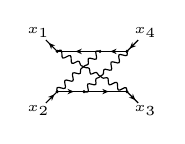
\begin{tikzpicture}[x=0.340cm, y=0.340cm, line width=0.420pt, baseline={([yshift=-0.6ex]0,0)}]
  \draw (0.300,0.750) -- (-1.300,0.750);
  \fill (-0.619,0.750) -- (-0.381,0.648) -- (-0.458,0.750) -- (-0.381,0.852) -- cycle;
  \draw (-0.300,-0.750) -- (1.300,-0.750);
  \fill (0.619,-0.750) -- (0.381,-0.648) -- (0.458,-0.750) -- (0.381,-0.852) -- cycle;
  \draw (-1.300,-0.750) -- (-0.300,-0.750);
  \fill (-0.681,-0.750) -- (-0.919,-0.648) -- (-0.842,-0.750) -- (-0.919,-0.852) -- cycle;
  \draw (1.300,0.750) -- (0.300,0.750);
  \fill (0.681,0.750) -- (0.919,0.648) -- (0.842,0.750) -- (0.919,0.852) -- cycle;
  \draw plot[smooth, tension=0.7] coordinates {(-1.300,0.750) (-1.218,0.791) (-1.159,0.794) (-1.132,0.741) (-1.127,0.650) (-1.122,0.559) (-1.094,0.506) (-1.035,0.509) (-0.953,0.550) (-0.872,0.591) (-0.813,0.594) (-0.785,0.541) (-0.780,0.450) (-0.775,0.359) (-0.747,0.306) (-0.688,0.309) (-0.607,0.350) (-0.529,0.385) (-0.479,0.370) (-0.456,0.312) (-0.433,0.250) (-0.396,0.214) (-0.349,0.196) (-0.303,0.175) (-0.260,0.150) (-0.209,0.139) (-0.151,0.138) (-0.107,0.116) (-0.087,0.050) (-0.079,-0.037) (-0.054,-0.094) (0.007,-0.087) (0.087,-0.050) (0.153,-0.034) (0.195,-0.062) (0.225,-0.111) (0.260,-0.150) (0.303,-0.175) (0.345,-0.204) (0.384,-0.236) (0.433,-0.250) (0.498,-0.238) (0.561,-0.230) (0.598,-0.265) (0.607,-0.350) (0.612,-0.441) (0.639,-0.494) (0.698,-0.491) (0.780,-0.450) (0.862,-0.409) (0.921,-0.406) (0.948,-0.459) (0.953,-0.550) (0.958,-0.641) (0.986,-0.694) (1.045,-0.691) (1.127,-0.650) (1.208,-0.609) (1.267,-0.606) (1.295,-0.659) (1.300,-0.750)};
  \draw plot[smooth, tension=0.7] coordinates {(-1.300,-0.750) (-1.316,-0.660) (-1.301,-0.603) (-1.243,-0.592) (-1.155,-0.614) (-1.066,-0.635) (-1.008,-0.624) (-0.993,-0.567) (-1.009,-0.477) (-1.025,-0.388) (-1.010,-0.331) (-0.952,-0.319) (-0.864,-0.341) (-0.775,-0.362) (-0.717,-0.351) (-0.702,-0.294) (-0.718,-0.205) (-0.734,-0.115) (-0.719,-0.058) (-0.661,-0.047) (-0.573,-0.068) (-0.487,-0.087) (-0.440,-0.064) (-0.431,-0.001) (-0.427,0.068) (-0.403,0.115) (-0.360,0.143) (-0.318,0.171) (-0.282,0.205) (-0.238,0.230) (-0.185,0.247) (-0.145,0.277) (-0.136,0.341) (-0.147,0.425) (-0.136,0.487) (-0.079,0.499) (0.009,0.477) (0.098,0.456) (0.155,0.467) (0.170,0.524) (0.155,0.614) (0.139,0.703) (0.154,0.760) (0.212,0.771) (0.300,0.750)};
  \draw plot[smooth, tension=0.7] coordinates {(1.300,0.750) (1.316,0.660) (1.301,0.603) (1.243,0.592) (1.155,0.614) (1.066,0.635) (1.008,0.624) (0.993,0.567) (1.009,0.477) (1.025,0.388) (1.010,0.331) (0.952,0.319) (0.864,0.341) (0.775,0.362) (0.717,0.351) (0.702,0.294) (0.718,0.205) (0.734,0.115) (0.719,0.058) (0.661,0.047) (0.573,0.068) (0.487,0.087) (0.440,0.064) (0.431,0.001) (0.427,-0.068) (0.403,-0.115) (0.360,-0.143) (0.318,-0.171) (0.282,-0.205) (0.238,-0.230) (0.185,-0.247) (0.145,-0.277) (0.136,-0.341) (0.147,-0.425) (0.136,-0.487) (0.079,-0.499) (-0.009,-0.477) (-0.098,-0.456) (-0.155,-0.467) (-0.170,-0.524) (-0.155,-0.614) (-0.139,-0.703) (-0.154,-0.760) (-0.212,-0.771) (-0.300,-0.750)};
  \draw (-1.300,0.750) -- (-1.724,1.174);
  \fill (-1.618,1.068) -- (-1.521,0.827) -- (-1.504,0.954) -- (-1.377,0.971) -- cycle;
  \draw (-1.300,-0.750) -- (-1.724,-1.174);
  \fill (-1.406,-0.856) -- (-1.647,-0.953) -- (-1.520,-0.970) -- (-1.503,-1.097) -- cycle;
  \draw (1.300,-0.750) -- (1.724,-1.174);
  \fill (1.618,-1.068) -- (1.521,-0.827) -- (1.504,-0.954) -- (1.377,-0.971) -- cycle;
  \draw (1.300,0.750) -- (1.724,1.174);
  \fill (1.406,0.856) -- (1.647,0.953) -- (1.520,0.970) -- (1.503,1.097) -- cycle;
  \fill (-1.300,0.750) circle (0.064);
  \fill (-1.300,-0.750) circle (0.064);
  \fill (1.300,-0.750) circle (0.064);
  \fill (1.300,0.750) circle (0.064);
  \fill (-0.300,-0.750) circle (0.064);
  \fill (0.300,0.750) circle (0.064);
  \node[font=\tiny, inner sep=0pt, anchor=315] at (-1.788,1.238) {$x_{1}$};
  \node[font=\tiny, inner sep=0pt, anchor=45] at (-1.788,-1.238) {$x_{2}$};
  \node[font=\tiny, inner sep=0pt, anchor=135] at (1.788,-1.238) {$x_{3}$};
  \node[font=\tiny, inner sep=0pt, anchor=225] at (1.788,1.238) {$x_{4}$};
\end{tikzpicture}}
\diagramgap
\mbox{$\displaystyle -\,$\,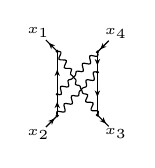
\begin{tikzpicture}[x=0.340cm, y=0.340cm, line width=0.420pt, baseline={([yshift=-0.6ex]0,0)}]
  \draw (-0.750,-0.404) -- (-0.750,1.196);
  \fill (-0.750,0.515) -- (-0.852,0.276) -- (-0.750,0.354) -- (-0.648,0.276) -- cycle;
  \draw (0.750,0.421) -- (0.750,-1.179);
  \fill (0.750,-0.499) -- (0.852,-0.260) -- (0.750,-0.337) -- (0.648,-0.260) -- cycle;
  \draw (-0.750,-1.204) -- (-0.750,-0.404);
  \fill (-0.750,-0.685) -- (-0.852,-0.924) -- (-0.750,-0.846) -- (-0.648,-0.924) -- cycle;
  \draw (0.750,1.171) -- (0.750,0.421);
  \fill (0.750,0.676) -- (0.852,0.915) -- (0.750,0.838) -- (0.648,0.915) -- cycle;
  \draw plot[smooth, tension=0.7] coordinates {(-0.750,1.196) (-0.665,1.194) (-0.614,1.171) (-0.615,1.115) (-0.650,1.038) (-0.685,0.960) (-0.686,0.904) (-0.635,0.881) (-0.550,0.879) (-0.465,0.878) (-0.414,0.854) (-0.415,0.799) (-0.450,0.721) (-0.485,0.643) (-0.486,0.588) (-0.435,0.564) (-0.350,0.563) (-0.265,0.561) (-0.218,0.535) (-0.225,0.475) (-0.250,0.404) (-0.252,0.348) (-0.221,0.312) (-0.180,0.282) (-0.150,0.246) (-0.123,0.207) (-0.088,0.174) (-0.056,0.139) (-0.050,0.088) (-0.069,0.020) (-0.070,-0.036) (-0.021,-0.061) (0.050,-0.071) (0.098,-0.096) (0.116,-0.140) (0.128,-0.188) (0.150,-0.229) (0.172,-0.271) (0.184,-0.319) (0.202,-0.362) (0.250,-0.387) (0.322,-0.397) (0.379,-0.417) (0.385,-0.468) (0.350,-0.546) (0.315,-0.624) (0.314,-0.679) (0.365,-0.703) (0.450,-0.704) (0.535,-0.706) (0.585,-0.729) (0.585,-0.785) (0.550,-0.862) (0.515,-0.940) (0.515,-0.996) (0.565,-1.019) (0.650,-1.021) (0.735,-1.022) (0.785,-1.046) (0.785,-1.101) (0.750,-1.179)};
  \draw plot[smooth, tension=0.7] coordinates {(-0.750,-1.204) (-0.772,-1.115) (-0.762,-1.057) (-0.704,-1.041) (-0.614,-1.056) (-0.523,-1.072) (-0.466,-1.056) (-0.455,-0.998) (-0.477,-0.909) (-0.500,-0.820) (-0.489,-0.761) (-0.431,-0.746) (-0.341,-0.761) (-0.250,-0.776) (-0.193,-0.761) (-0.182,-0.702) (-0.205,-0.613) (-0.227,-0.524) (-0.216,-0.466) (-0.159,-0.450) (-0.068,-0.466) (0.014,-0.473) (0.053,-0.441) (0.060,-0.379) (0.068,-0.318) (0.097,-0.276) (0.136,-0.243) (0.169,-0.206) (0.205,-0.170) (0.255,-0.149) (0.313,-0.133) (0.346,-0.096) (0.341,-0.022) (0.320,0.066) (0.329,0.125) (0.387,0.141) (0.477,0.125) (0.568,0.110) (0.625,0.126) (0.636,0.184) (0.614,0.273) (0.591,0.362) (0.602,0.421) (0.660,0.436) (0.750,0.421)};
  \draw plot[smooth, tension=0.7] coordinates {(0.750,1.171) (0.771,1.083) (0.759,1.026) (0.702,1.011) (0.614,1.028) (0.525,1.044) (0.468,1.030) (0.457,0.972) (0.477,0.884) (0.498,0.797) (0.486,0.739) (0.430,0.725) (0.341,0.741) (0.252,0.758) (0.195,0.743) (0.184,0.686) (0.205,0.598) (0.225,0.510) (0.214,0.453) (0.157,0.439) (0.068,0.455) (-0.010,0.461) (-0.048,0.429) (-0.057,0.369) (-0.068,0.312) (-0.098,0.272) (-0.136,0.240) (-0.168,0.202) (-0.205,0.169) (-0.257,0.150) (-0.315,0.137) (-0.348,0.100) (-0.341,0.025) (-0.321,-0.062) (-0.332,-0.120) (-0.389,-0.134) (-0.477,-0.118) (-0.566,-0.102) (-0.623,-0.116) (-0.634,-0.173) (-0.614,-0.261) (-0.593,-0.349) (-0.604,-0.406) (-0.661,-0.420) (-0.750,-0.404)};
  \draw (-0.750,1.196) -- (-1.174,1.620);
  \fill (-1.068,1.514) -- (-0.971,1.273) -- (-0.954,1.400) -- (-0.827,1.417) -- cycle;
  \draw (-0.750,-1.204) -- (-1.174,-1.628);
  \fill (-0.856,-1.311) -- (-1.097,-1.407) -- (-0.970,-1.425) -- (-0.953,-1.552) -- cycle;
  \draw (0.750,-1.179) -- (1.174,-1.603);
  \fill (1.068,-1.497) -- (0.971,-1.256) -- (0.954,-1.383) -- (0.827,-1.400) -- cycle;
  \draw (0.750,1.171) -- (1.174,1.595);
  \fill (0.856,1.277) -- (1.097,1.374) -- (0.970,1.391) -- (0.953,1.518) -- cycle;
  \fill (-0.750,1.196) circle (0.064);
  \fill (-0.750,-1.204) circle (0.064);
  \fill (0.750,-1.179) circle (0.064);
  \fill (0.750,1.171) circle (0.064);
  \fill (-0.750,-0.404) circle (0.064);
  \fill (0.750,0.421) circle (0.064);
  \node[font=\tiny, inner sep=0pt, anchor=315] at (-1.238,1.684) {$x_{1}$};
  \node[font=\tiny, inner sep=0pt, anchor=45] at (-1.238,-1.692) {$x_{2}$};
  \node[font=\tiny, inner sep=0pt, anchor=135] at (1.238,-1.667) {$x_{3}$};
  \node[font=\tiny, inner sep=0pt, anchor=225] at (1.238,1.659) {$x_{4}$};
\end{tikzpicture}}
\diagramgap
\mbox{$\displaystyle -\,$\,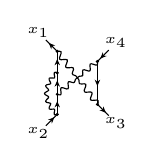
\begin{tikzpicture}[x=0.340cm, y=0.340cm, line width=0.420pt, baseline={([yshift=-0.6ex]0,0)}]
  \draw (-0.500,0.383) -- (-0.500,1.183);
  \fill (-0.500,0.903) -- (-0.602,0.664) -- (-0.500,0.742) -- (-0.398,0.664) -- cycle;
  \draw (1.000,0.808) -- (1.000,-0.792);
  \fill (1.000,-0.111) -- (1.102,0.128) -- (1.000,0.050) -- (0.898,0.128) -- cycle;
  \draw (-0.500,-1.167) -- (-0.500,-0.417);
  \fill (-0.500,-0.672) -- (-0.602,-0.911) -- (-0.500,-0.833) -- (-0.398,-0.911) -- cycle;
  \draw (-0.500,-0.417) -- (-0.500,0.383);
  \fill (-0.500,0.103) -- (-0.602,-0.136) -- (-0.500,-0.058) -- (-0.398,-0.136) -- cycle;
  \draw plot[smooth, tension=0.7] coordinates {(-0.500,1.183) (-0.413,1.189) (-0.360,1.170) (-0.355,1.113) (-0.385,1.031) (-0.414,0.949) (-0.409,0.893) (-0.356,0.873) (-0.269,0.879) (-0.182,0.886) (-0.129,0.866) (-0.125,0.810) (-0.154,0.728) (-0.183,0.646) (-0.178,0.589) (-0.125,0.570) (-0.038,0.576) (0.048,0.582) (0.101,0.562) (0.106,0.506) (0.077,0.424) (0.061,0.352) (0.087,0.311) (0.142,0.293) (0.192,0.272) (0.224,0.236) (0.250,0.196) (0.282,0.160) (0.308,0.120) (0.315,0.065) (0.318,0.008) (0.349,-0.028) (0.423,-0.032) (0.510,-0.026) (0.563,-0.046) (0.568,-0.102) (0.538,-0.184) (0.509,-0.266) (0.514,-0.322) (0.567,-0.342) (0.654,-0.336) (0.741,-0.330) (0.794,-0.350) (0.798,-0.406) (0.769,-0.488) (0.740,-0.570) (0.745,-0.626) (0.798,-0.646) (0.885,-0.640) (0.971,-0.634) (1.024,-0.653) (1.029,-0.710) (1.000,-0.792)};
  \draw plot[smooth, tension=0.7] coordinates {(-0.500,-1.167) (-0.559,-1.187) (-0.602,-1.181) (-0.616,-1.140) (-0.608,-1.078) (-0.596,-1.018) (-0.603,-0.980) (-0.641,-0.969) (-0.702,-0.975) (-0.764,-0.977) (-0.803,-0.959) (-0.805,-0.916) (-0.780,-0.859) (-0.751,-0.805) (-0.746,-0.766) (-0.779,-0.745) (-0.839,-0.733) (-0.900,-0.717) (-0.932,-0.688) (-0.921,-0.647) (-0.880,-0.599) (-0.836,-0.556) (-0.821,-0.520) (-0.846,-0.491) (-0.900,-0.461) (-0.954,-0.428) (-0.976,-0.392) (-0.954,-0.355) (-0.900,-0.322) (-0.846,-0.293) (-0.821,-0.263) (-0.836,-0.227) (-0.880,-0.184) (-0.921,-0.137) (-0.932,-0.095) (-0.900,-0.066) (-0.839,-0.050) (-0.779,-0.038) (-0.746,-0.017) (-0.751,0.021) (-0.780,0.076) (-0.805,0.133) (-0.803,0.176) (-0.764,0.194) (-0.702,0.192) (-0.641,0.186) (-0.603,0.196) (-0.596,0.235) (-0.608,0.295) (-0.616,0.357) (-0.602,0.397) (-0.559,0.404) (-0.500,0.383)};
  \draw plot[smooth, tension=0.7] coordinates {(1.000,0.808) (1.008,0.728) (0.992,0.679) (0.940,0.673) (0.864,0.697) (0.787,0.721) (0.735,0.715) (0.719,0.666) (0.727,0.586) (0.736,0.506) (0.719,0.456) (0.668,0.450) (0.591,0.474) (0.514,0.498) (0.463,0.492) (0.446,0.443) (0.455,0.363) (0.453,0.295) (0.421,0.264) (0.368,0.260) (0.318,0.252) (0.282,0.226) (0.250,0.196) (0.214,0.171) (0.182,0.140) (0.164,0.093) (0.149,0.042) (0.113,0.016) (0.045,0.029) (-0.031,0.053) (-0.083,0.047) (-0.099,-0.003) (-0.091,-0.083) (-0.082,-0.162) (-0.099,-0.212) (-0.151,-0.218) (-0.227,-0.194) (-0.304,-0.170) (-0.356,-0.176) (-0.372,-0.225) (-0.364,-0.305) (-0.355,-0.385) (-0.372,-0.435) (-0.423,-0.441) (-0.500,-0.417)};
  \draw (-0.500,1.183) -- (-0.924,1.608);
  \fill (-0.818,1.501) -- (-0.721,1.260) -- (-0.704,1.387) -- (-0.577,1.404) -- cycle;
  \draw (-0.500,-1.167) -- (-0.924,-1.591);
  \fill (-0.606,-1.273) -- (-0.847,-1.370) -- (-0.720,-1.387) -- (-0.703,-1.514) -- cycle;
  \draw (1.000,-0.792) -- (1.424,-1.216);
  \fill (1.318,-1.109) -- (1.221,-0.868) -- (1.204,-0.995) -- (1.077,-1.013) -- cycle;
  \draw (1.000,0.808) -- (1.424,1.233);
  \fill (1.106,0.915) -- (1.347,1.012) -- (1.220,1.029) -- (1.203,1.156) -- cycle;
  \fill (-0.500,1.183) circle (0.064);
  \fill (-0.500,-1.167) circle (0.064);
  \fill (1.000,-0.792) circle (0.064);
  \fill (1.000,0.808) circle (0.064);
  \fill (-0.500,-0.417) circle (0.064);
  \fill (-0.500,0.383) circle (0.064);
  \node[font=\tiny, inner sep=0pt, anchor=315] at (-0.988,1.671) {$x_{1}$};
  \node[font=\tiny, inner sep=0pt, anchor=45] at (-0.988,-1.655) {$x_{2}$};
  \node[font=\tiny, inner sep=0pt, anchor=135] at (1.488,-1.280) {$x_{3}$};
  \node[font=\tiny, inner sep=0pt, anchor=225] at (1.488,1.296) {$x_{4}$};
\end{tikzpicture}}
\diagramgap
\mbox{$\displaystyle +\,$\,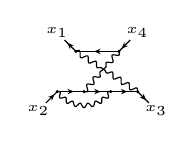
\begin{tikzpicture}[x=0.340cm, y=0.340cm, line width=0.420pt, baseline={([yshift=-0.6ex]0,0)}]
  \draw (0.800,1.000) -- (-0.800,1.000);
  \fill (-0.119,1.000) -- (0.119,0.898) -- (0.042,1.000) -- (0.119,1.102) -- cycle;
  \draw (0.500,-0.500) -- (1.500,-0.500);
  \fill (1.119,-0.500) -- (0.881,-0.398) -- (0.958,-0.500) -- (0.881,-0.602) -- cycle;
  \draw (-1.500,-0.500) -- (-0.500,-0.500);
  \fill (-0.881,-0.500) -- (-1.119,-0.398) -- (-1.042,-0.500) -- (-1.119,-0.602) -- cycle;
  \draw (-0.500,-0.500) -- (0.500,-0.500);
  \fill (0.119,-0.500) -- (-0.119,-0.398) -- (-0.042,-0.500) -- (-0.119,-0.602) -- cycle;
  \draw plot[smooth, tension=0.7] coordinates {(-0.800,1.000) (-0.723,1.034) (-0.669,1.033) (-0.647,0.984) (-0.647,0.900) (-0.647,0.816) (-0.624,0.767) (-0.570,0.766) (-0.493,0.800) (-0.417,0.834) (-0.363,0.833) (-0.340,0.784) (-0.340,0.700) (-0.340,0.616) (-0.317,0.567) (-0.263,0.566) (-0.187,0.600) (-0.110,0.634) (-0.056,0.633) (-0.033,0.584) (-0.033,0.500) (-0.029,0.423) (0.005,0.391) (0.062,0.395) (0.120,0.400) (0.164,0.383) (0.198,0.352) (0.235,0.325) (0.273,0.300) (0.302,0.261) (0.326,0.213) (0.363,0.187) (0.427,0.200) (0.502,0.231) (0.557,0.233) (0.580,0.184) (0.580,0.100) (0.580,0.016) (0.603,-0.033) (0.657,-0.034) (0.733,0.000) (0.810,0.034) (0.864,0.033) (0.887,-0.016) (0.887,-0.100) (0.887,-0.184) (0.909,-0.233) (0.963,-0.234) (1.040,-0.200) (1.117,-0.166) (1.171,-0.167) (1.193,-0.216) (1.193,-0.300) (1.193,-0.384) (1.216,-0.433) (1.270,-0.434) (1.347,-0.400) (1.423,-0.366) (1.477,-0.367) (1.500,-0.416) (1.500,-0.500)};
  \draw plot[smooth, tension=0.7] coordinates {(-1.500,-0.500) (-1.431,-0.497) (-1.390,-0.512) (-1.385,-0.555) (-1.402,-0.622) (-1.417,-0.690) (-1.404,-0.736) (-1.358,-0.747) (-1.290,-0.730) (-1.224,-0.710) (-1.180,-0.714) (-1.164,-0.754) (-1.165,-0.823) (-1.161,-0.893) (-1.138,-0.934) (-1.090,-0.933) (-1.029,-0.900) (-0.970,-0.863) (-0.927,-0.856) (-0.901,-0.891) (-0.884,-0.958) (-0.863,-1.025) (-0.830,-1.059) (-0.784,-1.046) (-0.733,-0.998) (-0.685,-0.948) (-0.645,-0.929) (-0.611,-0.957) (-0.578,-1.018) (-0.541,-1.077) (-0.500,-1.101) (-0.459,-1.077) (-0.422,-1.018) (-0.389,-0.957) (-0.355,-0.929) (-0.315,-0.948) (-0.267,-0.998) (-0.216,-1.046) (-0.170,-1.059) (-0.137,-1.025) (-0.116,-0.958) (-0.099,-0.891) (-0.073,-0.856) (-0.030,-0.863) (0.029,-0.900) (0.090,-0.933) (0.138,-0.934) (0.161,-0.893) (0.165,-0.823) (0.164,-0.754) (0.180,-0.714) (0.224,-0.710) (0.290,-0.730) (0.358,-0.747) (0.404,-0.736) (0.417,-0.690) (0.402,-0.622) (0.385,-0.555) (0.390,-0.512) (0.431,-0.497) (0.500,-0.500)};
  \draw plot[smooth, tension=0.7] coordinates {(0.800,1.000) (0.823,0.921) (0.815,0.868) (0.763,0.853) (0.682,0.864) (0.600,0.875) (0.549,0.859) (0.541,0.806) (0.564,0.727) (0.586,0.648) (0.578,0.595) (0.527,0.580) (0.445,0.591) (0.365,0.601) (0.322,0.578) (0.321,0.520) (0.327,0.455) (0.313,0.407) (0.277,0.379) (0.240,0.352) (0.209,0.318) (0.174,0.289) (0.130,0.267) (0.096,0.237) (0.091,0.182) (0.106,0.109) (0.103,0.052) (0.054,0.034) (-0.027,0.045) (-0.109,0.056) (-0.160,0.041) (-0.168,-0.012) (-0.145,-0.091) (-0.123,-0.170) (-0.131,-0.223) (-0.182,-0.238) (-0.264,-0.227) (-0.345,-0.216) (-0.396,-0.232) (-0.404,-0.284) (-0.382,-0.364) (-0.359,-0.443) (-0.367,-0.496) (-0.418,-0.511) (-0.500,-0.500)};
  \draw (-0.800,1.000) -- (-1.224,1.424);
  \fill (-1.118,1.318) -- (-1.021,1.077) -- (-1.004,1.204) -- (-0.877,1.221) -- cycle;
  \draw (-1.500,-0.500) -- (-1.924,-0.924);
  \fill (-1.606,-0.606) -- (-1.847,-0.703) -- (-1.720,-0.720) -- (-1.703,-0.847) -- cycle;
  \draw (1.500,-0.500) -- (1.924,-0.924);
  \fill (1.818,-0.818) -- (1.721,-0.577) -- (1.704,-0.704) -- (1.577,-0.721) -- cycle;
  \draw (0.800,1.000) -- (1.224,1.424);
  \fill (0.906,1.106) -- (1.147,1.203) -- (1.020,1.220) -- (1.003,1.347) -- cycle;
  \fill (-0.800,1.000) circle (0.064);
  \fill (-1.500,-0.500) circle (0.064);
  \fill (1.500,-0.500) circle (0.064);
  \fill (0.800,1.000) circle (0.064);
  \fill (-0.500,-0.500) circle (0.064);
  \fill (0.500,-0.500) circle (0.064);
  \node[font=\tiny, inner sep=0pt, anchor=315] at (-1.288,1.488) {$x_{1}$};
  \node[font=\tiny, inner sep=0pt, anchor=45] at (-1.988,-0.988) {$x_{2}$};
  \node[font=\tiny, inner sep=0pt, anchor=135] at (1.988,-0.988) {$x_{3}$};
  \node[font=\tiny, inner sep=0pt, anchor=225] at (1.288,1.488) {$x_{4}$};
\end{tikzpicture}}
\diagramgap
\mbox{$\displaystyle +\,$\,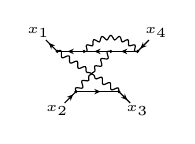
\begin{tikzpicture}[x=0.340cm, y=0.340cm, line width=0.420pt, baseline={([yshift=-0.6ex]0,0)}]
  \draw (-0.500,0.500) -- (-1.500,0.500);
  \fill (-1.119,0.500) -- (-0.881,0.398) -- (-0.958,0.500) -- (-0.881,0.602) -- cycle;
  \draw (-0.800,-1.000) -- (0.800,-1.000);
  \fill (0.119,-1.000) -- (-0.119,-0.898) -- (-0.042,-1.000) -- (-0.119,-1.102) -- cycle;
  \draw (1.500,0.500) -- (0.500,0.500);
  \fill (0.881,0.500) -- (1.119,0.398) -- (1.042,0.500) -- (1.119,0.602) -- cycle;
  \draw (0.500,0.500) -- (-0.500,0.500);
  \fill (-0.119,0.500) -- (0.119,0.398) -- (0.042,0.500) -- (0.119,0.602) -- cycle;
  \draw plot[smooth, tension=0.7] coordinates {(-1.500,0.500) (-1.423,0.534) (-1.369,0.533) (-1.347,0.484) (-1.347,0.400) (-1.347,0.316) (-1.324,0.267) (-1.270,0.266) (-1.193,0.300) (-1.117,0.334) (-1.063,0.333) (-1.040,0.284) (-1.040,0.200) (-1.040,0.116) (-1.017,0.067) (-0.963,0.066) (-0.887,0.100) (-0.810,0.134) (-0.756,0.133) (-0.733,0.084) (-0.733,0.000) (-0.733,-0.084) (-0.711,-0.133) (-0.657,-0.134) (-0.580,-0.100) (-0.503,-0.066) (-0.449,-0.067) (-0.428,-0.119) (-0.427,-0.200) (-0.413,-0.263) (-0.374,-0.287) (-0.321,-0.289) (-0.273,-0.300) (-0.235,-0.325) (-0.195,-0.348) (-0.153,-0.367) (-0.120,-0.400) (-0.101,-0.455) (-0.082,-0.509) (-0.039,-0.527) (0.033,-0.500) (0.110,-0.466) (0.164,-0.467) (0.187,-0.516) (0.187,-0.600) (0.187,-0.684) (0.209,-0.733) (0.263,-0.734) (0.340,-0.700) (0.417,-0.666) (0.471,-0.667) (0.493,-0.716) (0.493,-0.800) (0.493,-0.884) (0.516,-0.933) (0.570,-0.934) (0.647,-0.900) (0.723,-0.866) (0.777,-0.867) (0.800,-0.916) (0.800,-1.000)};
  \draw plot[smooth, tension=0.7] coordinates {(-0.800,-1.000) (-0.823,-0.921) (-0.815,-0.868) (-0.763,-0.853) (-0.682,-0.864) (-0.600,-0.875) (-0.549,-0.859) (-0.541,-0.806) (-0.564,-0.727) (-0.586,-0.648) (-0.578,-0.595) (-0.527,-0.580) (-0.445,-0.591) (-0.365,-0.601) (-0.322,-0.578) (-0.321,-0.520) (-0.327,-0.455) (-0.313,-0.407) (-0.277,-0.379) (-0.240,-0.352) (-0.209,-0.318) (-0.174,-0.289) (-0.130,-0.267) (-0.096,-0.237) (-0.091,-0.182) (-0.106,-0.109) (-0.103,-0.052) (-0.054,-0.034) (0.027,-0.045) (0.109,-0.056) (0.160,-0.041) (0.168,0.012) (0.145,0.091) (0.123,0.170) (0.131,0.223) (0.182,0.238) (0.264,0.227) (0.345,0.216) (0.396,0.232) (0.404,0.284) (0.382,0.364) (0.359,0.443) (0.367,0.496) (0.418,0.511) (0.500,0.500)};
  \draw plot[smooth, tension=0.7] coordinates {(1.500,0.500) (1.431,0.497) (1.390,0.512) (1.385,0.555) (1.402,0.622) (1.417,0.690) (1.404,0.736) (1.358,0.747) (1.290,0.730) (1.224,0.710) (1.180,0.714) (1.164,0.754) (1.165,0.823) (1.161,0.893) (1.138,0.934) (1.090,0.933) (1.029,0.900) (0.970,0.863) (0.927,0.856) (0.901,0.891) (0.884,0.958) (0.863,1.025) (0.830,1.059) (0.784,1.046) (0.733,0.998) (0.685,0.948) (0.645,0.929) (0.611,0.957) (0.578,1.018) (0.541,1.077) (0.500,1.101) (0.459,1.077) (0.422,1.018) (0.389,0.957) (0.355,0.929) (0.315,0.948) (0.267,0.998) (0.216,1.046) (0.170,1.059) (0.137,1.025) (0.116,0.958) (0.099,0.891) (0.073,0.856) (0.030,0.863) (-0.029,0.900) (-0.090,0.933) (-0.138,0.934) (-0.161,0.893) (-0.165,0.823) (-0.164,0.754) (-0.180,0.714) (-0.224,0.710) (-0.290,0.730) (-0.358,0.747) (-0.404,0.736) (-0.417,0.690) (-0.402,0.622) (-0.385,0.555) (-0.390,0.512) (-0.431,0.497) (-0.500,0.500)};
  \draw (-1.500,0.500) -- (-1.924,0.924);
  \fill (-1.818,0.818) -- (-1.721,0.577) -- (-1.704,0.704) -- (-1.577,0.721) -- cycle;
  \draw (-0.800,-1.000) -- (-1.224,-1.424);
  \fill (-0.906,-1.106) -- (-1.147,-1.203) -- (-1.020,-1.220) -- (-1.003,-1.347) -- cycle;
  \draw (0.800,-1.000) -- (1.224,-1.424);
  \fill (1.118,-1.318) -- (1.021,-1.077) -- (1.004,-1.204) -- (0.877,-1.221) -- cycle;
  \draw (1.500,0.500) -- (1.924,0.924);
  \fill (1.606,0.606) -- (1.847,0.703) -- (1.720,0.720) -- (1.703,0.847) -- cycle;
  \fill (-1.500,0.500) circle (0.064);
  \fill (-0.800,-1.000) circle (0.064);
  \fill (0.800,-1.000) circle (0.064);
  \fill (1.500,0.500) circle (0.064);
  \fill (0.500,0.500) circle (0.064);
  \fill (-0.500,0.500) circle (0.064);
  \node[font=\tiny, inner sep=0pt, anchor=315] at (-1.988,0.988) {$x_{1}$};
  \node[font=\tiny, inner sep=0pt, anchor=45] at (-1.288,-1.488) {$x_{2}$};
  \node[font=\tiny, inner sep=0pt, anchor=135] at (1.288,-1.488) {$x_{3}$};
  \node[font=\tiny, inner sep=0pt, anchor=225] at (1.988,0.988) {$x_{4}$};
\end{tikzpicture}}
\diagramgap
\mbox{$\displaystyle -\,$\,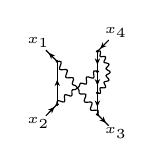
\begin{tikzpicture}[x=0.340cm, y=0.340cm, line width=0.420pt, baseline={([yshift=-0.6ex]0,0)}]
  \draw (-1.000,-0.808) -- (-1.000,0.792);
  \fill (-1.000,0.111) -- (-1.102,-0.128) -- (-1.000,-0.050) -- (-0.898,-0.128) -- cycle;
  \draw (0.500,-0.383) -- (0.500,-1.183);
  \fill (0.500,-0.903) -- (0.602,-0.664) -- (0.500,-0.742) -- (0.398,-0.664) -- cycle;
  \draw (0.500,1.167) -- (0.500,0.417);
  \fill (0.500,0.672) -- (0.602,0.911) -- (0.500,0.833) -- (0.398,0.911) -- cycle;
  \draw (0.500,0.417) -- (0.500,-0.383);
  \fill (0.500,-0.103) -- (0.602,0.136) -- (0.500,0.058) -- (0.398,0.136) -- cycle;
  \draw plot[smooth, tension=0.7] coordinates {(-1.000,0.792) (-0.913,0.798) (-0.860,0.778) (-0.855,0.722) (-0.885,0.640) (-0.914,0.558) (-0.909,0.501) (-0.856,0.482) (-0.769,0.488) (-0.682,0.494) (-0.630,0.474) (-0.625,0.418) (-0.654,0.336) (-0.683,0.254) (-0.678,0.198) (-0.625,0.178) (-0.538,0.184) (-0.452,0.190) (-0.399,0.170) (-0.394,0.114) (-0.423,0.032) (-0.439,-0.040) (-0.413,-0.080) (-0.358,-0.098) (-0.308,-0.120) (-0.276,-0.156) (-0.250,-0.196) (-0.218,-0.232) (-0.192,-0.272) (-0.185,-0.326) (-0.182,-0.384) (-0.151,-0.420) (-0.077,-0.424) (0.010,-0.418) (0.063,-0.437) (0.068,-0.494) (0.038,-0.576) (0.009,-0.658) (0.014,-0.714) (0.067,-0.734) (0.154,-0.728) (0.241,-0.721) (0.294,-0.741) (0.298,-0.797) (0.269,-0.879) (0.240,-0.962) (0.245,-1.018) (0.298,-1.037) (0.385,-1.031) (0.471,-1.025) (0.524,-1.045) (0.529,-1.101) (0.500,-1.183)};
  \draw plot[smooth, tension=0.7] coordinates {(-1.000,-0.808) (-1.008,-0.728) (-0.992,-0.679) (-0.940,-0.673) (-0.864,-0.697) (-0.787,-0.721) (-0.735,-0.715) (-0.719,-0.666) (-0.727,-0.586) (-0.736,-0.506) (-0.719,-0.456) (-0.668,-0.450) (-0.591,-0.474) (-0.514,-0.498) (-0.463,-0.492) (-0.446,-0.443) (-0.455,-0.363) (-0.453,-0.295) (-0.421,-0.264) (-0.368,-0.260) (-0.318,-0.252) (-0.282,-0.226) (-0.250,-0.196) (-0.214,-0.171) (-0.182,-0.140) (-0.164,-0.093) (-0.149,-0.042) (-0.113,-0.016) (-0.045,-0.029) (0.031,-0.053) (0.083,-0.047) (0.099,0.003) (0.091,0.083) (0.082,0.162) (0.099,0.212) (0.151,0.218) (0.227,0.194) (0.304,0.170) (0.356,0.176) (0.372,0.225) (0.364,0.305) (0.355,0.385) (0.372,0.435) (0.423,0.441) (0.500,0.417)};
  \draw plot[smooth, tension=0.7] coordinates {(0.500,1.167) (0.559,1.187) (0.602,1.181) (0.616,1.140) (0.608,1.078) (0.596,1.018) (0.603,0.980) (0.641,0.969) (0.702,0.975) (0.764,0.977) (0.803,0.959) (0.805,0.916) (0.780,0.859) (0.751,0.805) (0.746,0.766) (0.779,0.745) (0.839,0.733) (0.900,0.717) (0.932,0.688) (0.921,0.647) (0.880,0.599) (0.836,0.556) (0.821,0.520) (0.846,0.491) (0.900,0.461) (0.954,0.428) (0.976,0.392) (0.954,0.355) (0.900,0.322) (0.846,0.293) (0.821,0.263) (0.836,0.227) (0.880,0.184) (0.921,0.137) (0.932,0.095) (0.900,0.066) (0.839,0.050) (0.779,0.038) (0.746,0.017) (0.751,-0.021) (0.780,-0.076) (0.805,-0.133) (0.803,-0.176) (0.764,-0.194) (0.702,-0.192) (0.641,-0.186) (0.603,-0.196) (0.596,-0.235) (0.608,-0.295) (0.616,-0.357) (0.602,-0.397) (0.559,-0.404) (0.500,-0.383)};
  \draw (-1.000,0.792) -- (-1.424,1.216);
  \fill (-1.318,1.109) -- (-1.221,0.868) -- (-1.204,0.995) -- (-1.077,1.013) -- cycle;
  \draw (-1.000,-0.808) -- (-1.424,-1.233);
  \fill (-1.106,-0.915) -- (-1.347,-1.012) -- (-1.220,-1.029) -- (-1.203,-1.156) -- cycle;
  \draw (0.500,-1.183) -- (0.924,-1.608);
  \fill (0.818,-1.501) -- (0.721,-1.260) -- (0.704,-1.387) -- (0.577,-1.404) -- cycle;
  \draw (0.500,1.167) -- (0.924,1.591);
  \fill (0.606,1.273) -- (0.847,1.370) -- (0.720,1.387) -- (0.703,1.514) -- cycle;
  \fill (-1.000,0.792) circle (0.064);
  \fill (-1.000,-0.808) circle (0.064);
  \fill (0.500,-1.183) circle (0.064);
  \fill (0.500,1.167) circle (0.064);
  \fill (0.500,0.417) circle (0.064);
  \fill (0.500,-0.383) circle (0.064);
  \node[font=\tiny, inner sep=0pt, anchor=315] at (-1.488,1.280) {$x_{1}$};
  \node[font=\tiny, inner sep=0pt, anchor=45] at (-1.488,-1.296) {$x_{2}$};
  \node[font=\tiny, inner sep=0pt, anchor=135] at (0.988,-1.671) {$x_{3}$};
  \node[font=\tiny, inner sep=0pt, anchor=225] at (0.988,1.655) {$x_{4}$};
\end{tikzpicture}}
\diagramgap
\mbox{$\displaystyle -\,$\,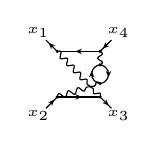
\begin{tikzpicture}[x=0.340cm, y=0.340cm, line width=0.420pt, baseline={([yshift=-0.6ex]0,0)}]
  \draw (0.533,0.850) -- (-1.067,0.850);
  \fill (-0.386,0.850) -- (-0.147,0.748) -- (-0.225,0.850) -- (-0.147,0.952) -- cycle;
  \draw (-1.067,-0.850) -- (0.533,-0.850);
  \fill (-0.147,-0.850) -- (-0.386,-0.748) -- (-0.308,-0.850) -- (-0.386,-0.952) -- cycle;
  \draw (0.533,0.350) arc[start angle=83.974, end angle=-83.974, radius=0.352];
  \fill (0.848,-0.119) -- (0.950,0.119) -- (0.848,0.042) -- (0.746,0.119) -- cycle;
  \draw (0.533,-0.350) arc[start angle=263.974, end angle=96.026, radius=0.352];
  \fill (0.218,0.119) -- (0.116,-0.119) -- (0.218,-0.042) -- (0.320,-0.119) -- cycle;
  \draw plot[smooth, tension=0.7] coordinates {(-1.067,0.850) (-0.986,0.864) (-0.935,0.851) (-0.924,0.799) (-0.944,0.719) (-0.963,0.640) (-0.953,0.587) (-0.901,0.574) (-0.821,0.588) (-0.740,0.603) (-0.688,0.590) (-0.678,0.537) (-0.697,0.458) (-0.717,0.378) (-0.707,0.326) (-0.655,0.313) (-0.574,0.327) (-0.494,0.341) (-0.442,0.328) (-0.432,0.276) (-0.451,0.196) (-0.470,0.116) (-0.460,0.064) (-0.409,0.051) (-0.328,0.065) (-0.248,0.080) (-0.196,0.066) (-0.186,0.014) (-0.205,-0.065) (-0.224,-0.145) (-0.214,-0.197) (-0.163,-0.210) (-0.082,-0.196) (-0.001,-0.182) (0.046,-0.199) (0.051,-0.256) (0.041,-0.327) (0.051,-0.379) (0.087,-0.407) (0.130,-0.428) (0.164,-0.458) (0.197,-0.489) (0.237,-0.513) (0.273,-0.540) (0.287,-0.588) (0.281,-0.656) (0.285,-0.714) (0.330,-0.733) (0.410,-0.719) (0.491,-0.705) (0.542,-0.718) (0.552,-0.770) (0.533,-0.850)};
  \draw plot[smooth, tension=0.7] coordinates {(-1.067,-0.850) (-1.043,-0.768) (-1.008,-0.726) (-0.955,-0.740) (-0.889,-0.794) (-0.823,-0.848) (-0.770,-0.863) (-0.734,-0.821) (-0.711,-0.739) (-0.688,-0.657) (-0.652,-0.615) (-0.599,-0.629) (-0.533,-0.683) (-0.468,-0.737) (-0.414,-0.752) (-0.379,-0.710) (-0.356,-0.628) (-0.332,-0.546) (-0.297,-0.504) (-0.243,-0.518) (-0.178,-0.572) (-0.112,-0.626) (-0.062,-0.631) (-0.029,-0.581) (0.000,-0.517) (0.037,-0.480) (0.084,-0.474) (0.133,-0.473) (0.178,-0.461) (0.224,-0.452) (0.273,-0.454) (0.320,-0.447) (0.356,-0.406) (0.383,-0.337) (0.416,-0.287) (0.468,-0.296) (0.533,-0.350)};
  \draw plot[smooth, tension=0.7] coordinates {(0.533,0.850) (0.597,0.808) (0.623,0.767) (0.597,0.725) (0.533,0.683) (0.470,0.642) (0.443,0.600) (0.470,0.558) (0.533,0.517) (0.597,0.475) (0.623,0.433) (0.597,0.392) (0.533,0.350)};
  \draw (-1.067,0.850) -- (-1.491,1.274);
  \fill (-1.384,1.168) -- (-1.288,0.927) -- (-1.270,1.054) -- (-1.143,1.071) -- cycle;
  \draw (-1.067,-0.850) -- (-1.491,-1.274);
  \fill (-1.173,-0.956) -- (-1.414,-1.053) -- (-1.287,-1.070) -- (-1.270,-1.197) -- cycle;
  \draw (0.533,-0.850) -- (0.958,-1.274);
  \fill (0.851,-1.168) -- (0.754,-0.927) -- (0.737,-1.054) -- (0.610,-1.071) -- cycle;
  \draw (0.533,0.850) -- (0.958,1.274);
  \fill (0.640,0.956) -- (0.881,1.053) -- (0.754,1.070) -- (0.737,1.197) -- cycle;
  \fill (-1.067,0.850) circle (0.064);
  \fill (-1.067,-0.850) circle (0.064);
  \fill (0.533,-0.850) circle (0.064);
  \fill (0.533,0.850) circle (0.064);
  \fill (0.533,-0.350) circle (0.064);
  \fill (0.533,0.350) circle (0.064);
  \node[font=\tiny, inner sep=0pt, anchor=315] at (-1.555,1.338) {$x_{1}$};
  \node[font=\tiny, inner sep=0pt, anchor=45] at (-1.555,-1.338) {$x_{2}$};
  \node[font=\tiny, inner sep=0pt, anchor=135] at (1.021,-1.338) {$x_{3}$};
  \node[font=\tiny, inner sep=0pt, anchor=225] at (1.021,1.338) {$x_{4}$};
\end{tikzpicture}}
\diagramgap
\mbox{$\displaystyle +\,$\,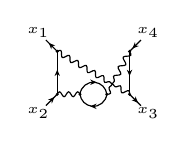
\begin{tikzpicture}[x=0.340cm, y=0.340cm, line width=0.420pt, baseline={([yshift=-0.6ex]0,0)}]
  \draw (-1.350,-0.533) -- (-1.350,1.067);
  \fill (-1.350,0.386) -- (-1.452,0.147) -- (-1.350,0.225) -- (-1.248,0.147) -- cycle;
  \draw (1.350,1.067) -- (1.350,-0.533);
  \fill (1.350,0.147) -- (1.452,0.386) -- (1.350,0.308) -- (1.248,0.386) -- cycle;
  \draw (0.500,-0.533) arc[start angle=353.974, end angle=186.026, radius=0.503];
  \fill (-0.119,-0.983) -- (0.119,-1.085) -- (0.042,-0.983) -- (0.119,-0.881) -- cycle;
  \draw (-0.500,-0.533) arc[start angle=173.974, end angle=6.026, radius=0.503];
  \fill (0.119,-0.083) -- (-0.119,0.019) -- (-0.042,-0.083) -- (-0.119,-0.185) -- cycle;
  \draw plot[smooth, tension=0.7] coordinates {(-1.350,1.067) (-1.274,1.104) (-1.220,1.105) (-1.195,1.057) (-1.191,0.973) (-1.187,0.888) (-1.163,0.840) (-1.108,0.841) (-1.032,0.878) (-0.957,0.916) (-0.902,0.917) (-0.877,0.868) (-0.874,0.784) (-0.870,0.700) (-0.845,0.651) (-0.790,0.653) (-0.715,0.690) (-0.639,0.727) (-0.584,0.729) (-0.560,0.680) (-0.556,0.596) (-0.552,0.512) (-0.527,0.463) (-0.473,0.465) (-0.397,0.502) (-0.321,0.539) (-0.267,0.541) (-0.242,0.492) (-0.238,0.408) (-0.234,0.324) (-0.210,0.275) (-0.155,0.277) (-0.079,0.314) (-0.004,0.351) (0.051,0.352) (0.076,0.304) (0.079,0.220) (0.083,0.135) (0.108,0.087) (0.163,0.088) (0.238,0.125) (0.314,0.163) (0.368,0.164) (0.393,0.116) (0.397,0.031) (0.401,-0.052) (0.431,-0.092) (0.490,-0.083) (0.556,-0.063) (0.607,-0.067) (0.643,-0.097) (0.676,-0.132) (0.715,-0.157) (0.751,-0.185) (0.782,-0.224) (0.818,-0.254) (0.874,-0.251) (0.943,-0.224) (1.001,-0.216) (1.029,-0.261) (1.032,-0.345) (1.036,-0.429) (1.061,-0.478) (1.116,-0.476) (1.191,-0.439) (1.267,-0.402) (1.321,-0.401) (1.346,-0.449) (1.350,-0.533)};
  \draw plot[smooth, tension=0.7] coordinates {(-1.350,-0.533) (-1.308,-0.468) (-1.265,-0.442) (-1.223,-0.468) (-1.180,-0.533) (-1.138,-0.598) (-1.095,-0.625) (-1.052,-0.598) (-1.010,-0.533) (-0.968,-0.468) (-0.925,-0.442) (-0.883,-0.468) (-0.840,-0.533) (-0.798,-0.598) (-0.755,-0.625) (-0.713,-0.598) (-0.670,-0.533) (-0.628,-0.468) (-0.585,-0.442) (-0.543,-0.468) (-0.500,-0.533)};
  \draw plot[smooth, tension=0.7] coordinates {(1.350,1.067) (1.394,0.986) (1.399,0.927) (1.347,0.897) (1.256,0.889) (1.164,0.881) (1.112,0.851) (1.117,0.792) (1.161,0.711) (1.205,0.631) (1.210,0.571) (1.158,0.542) (1.067,0.533) (0.975,0.525) (0.923,0.495) (0.928,0.436) (0.972,0.356) (1.016,0.275) (1.021,0.216) (0.969,0.186) (0.878,0.178) (0.789,0.168) (0.750,0.132) (0.762,0.068) (0.783,0.000) (0.777,-0.054) (0.745,-0.094) (0.713,-0.134) (0.689,-0.178) (0.657,-0.218) (0.613,-0.251) (0.584,-0.293) (0.594,-0.356) (0.630,-0.432) (0.641,-0.495) (0.591,-0.525) (0.500,-0.533)};
  \draw (-1.350,1.067) -- (-1.774,1.491);
  \fill (-1.668,1.384) -- (-1.571,1.143) -- (-1.554,1.270) -- (-1.427,1.288) -- cycle;
  \draw (-1.350,-0.533) -- (-1.774,-0.958);
  \fill (-1.456,-0.640) -- (-1.697,-0.737) -- (-1.570,-0.754) -- (-1.553,-0.881) -- cycle;
  \draw (1.350,-0.533) -- (1.774,-0.958);
  \fill (1.668,-0.851) -- (1.571,-0.610) -- (1.554,-0.737) -- (1.427,-0.754) -- cycle;
  \draw (1.350,1.067) -- (1.774,1.491);
  \fill (1.456,1.173) -- (1.697,1.270) -- (1.570,1.287) -- (1.553,1.414) -- cycle;
  \fill (-1.350,1.067) circle (0.064);
  \fill (-1.350,-0.533) circle (0.064);
  \fill (1.350,-0.533) circle (0.064);
  \fill (1.350,1.067) circle (0.064);
  \fill (-0.500,-0.533) circle (0.064);
  \fill (0.500,-0.533) circle (0.064);
  \node[font=\tiny, inner sep=0pt, anchor=315] at (-1.838,1.555) {$x_{1}$};
  \node[font=\tiny, inner sep=0pt, anchor=45] at (-1.838,-1.021) {$x_{2}$};
  \node[font=\tiny, inner sep=0pt, anchor=135] at (1.838,-1.021) {$x_{3}$};
  \node[font=\tiny, inner sep=0pt, anchor=225] at (1.838,1.555) {$x_{4}$};
\end{tikzpicture}}
\diagramgap
\mbox{$\displaystyle -\,$\,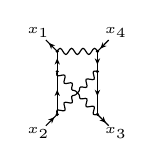
\begin{tikzpicture}[x=0.340cm, y=0.340cm, line width=0.420pt, baseline={([yshift=-0.6ex]0,0)}]
  \draw (-0.750,0.283) -- (-0.750,1.033);
  \fill (-0.750,0.778) -- (-0.852,0.539) -- (-0.750,0.617) -- (-0.648,0.539) -- cycle;
  \draw (0.750,0.283) -- (0.750,-1.317);
  \fill (0.750,-0.636) -- (0.852,-0.397) -- (0.750,-0.475) -- (0.648,-0.397) -- cycle;
  \draw (-0.750,-1.317) -- (-0.750,0.283);
  \fill (-0.750,-0.397) -- (-0.852,-0.636) -- (-0.750,-0.558) -- (-0.648,-0.636) -- cycle;
  \draw (0.750,1.033) -- (0.750,0.283);
  \fill (0.750,0.539) -- (0.852,0.778) -- (0.750,0.700) -- (0.648,0.778) -- cycle;
  \draw plot[smooth, tension=0.7] coordinates {(-0.750,1.033) (-0.696,1.115) (-0.643,1.149) (-0.589,1.115) (-0.536,1.033) (-0.482,0.952) (-0.429,0.918) (-0.375,0.952) (-0.321,1.033) (-0.268,1.115) (-0.214,1.149) (-0.161,1.115) (-0.107,1.033) (-0.054,0.952) (0.000,0.918) (0.054,0.952) (0.107,1.033) (0.161,1.115) (0.214,1.149) (0.268,1.115) (0.321,1.033) (0.375,0.952) (0.429,0.918) (0.482,0.952) (0.536,1.033) (0.589,1.115) (0.643,1.149) (0.696,1.115) (0.750,1.033)};
  \draw plot[smooth, tension=0.7] coordinates {(-0.750,-1.317) (-0.771,-1.228) (-0.760,-1.170) (-0.703,-1.156) (-0.614,-1.171) (-0.524,-1.187) (-0.467,-1.172) (-0.456,-1.114) (-0.477,-1.026) (-0.499,-0.937) (-0.488,-0.879) (-0.431,-0.865) (-0.341,-0.880) (-0.251,-0.896) (-0.194,-0.881) (-0.183,-0.823) (-0.205,-0.735) (-0.214,-0.658) (-0.182,-0.619) (-0.123,-0.606) (-0.068,-0.589) (-0.031,-0.556) (0.000,-0.517) (0.037,-0.483) (0.068,-0.444) (0.081,-0.388) (0.091,-0.328) (0.127,-0.294) (0.205,-0.298) (0.294,-0.314) (0.351,-0.299) (0.362,-0.241) (0.341,-0.153) (0.319,-0.065) (0.331,-0.007) (0.388,0.008) (0.477,-0.008) (0.567,-0.023) (0.624,-0.008) (0.635,0.049) (0.614,0.138) (0.592,0.226) (0.603,0.284) (0.660,0.299) (0.750,0.283)};
  \draw plot[smooth, tension=0.7] coordinates {(0.750,-1.317) (0.660,-1.332) (0.603,-1.318) (0.592,-1.260) (0.614,-1.171) (0.635,-1.083) (0.624,-1.025) (0.567,-1.010) (0.477,-1.026) (0.388,-1.041) (0.331,-1.027) (0.319,-0.969) (0.341,-0.880) (0.362,-0.792) (0.351,-0.734) (0.294,-0.719) (0.205,-0.735) (0.127,-0.739) (0.091,-0.705) (0.081,-0.645) (0.068,-0.589) (0.037,-0.550) (0.000,-0.517) (-0.031,-0.478) (-0.068,-0.444) (-0.123,-0.427) (-0.182,-0.414) (-0.214,-0.375) (-0.205,-0.298) (-0.183,-0.210) (-0.194,-0.152) (-0.251,-0.137) (-0.341,-0.153) (-0.431,-0.169) (-0.488,-0.154) (-0.499,-0.096) (-0.477,-0.008) (-0.456,0.081) (-0.467,0.139) (-0.524,0.154) (-0.614,0.138) (-0.703,0.122) (-0.760,0.137) (-0.771,0.195) (-0.750,0.283)};
  \draw (-0.750,1.033) -- (-1.174,1.458);
  \fill (-1.068,1.351) -- (-0.971,1.110) -- (-0.954,1.237) -- (-0.827,1.254) -- cycle;
  \draw (-0.750,-1.317) -- (-1.174,-1.741);
  \fill (-0.856,-1.423) -- (-1.097,-1.520) -- (-0.970,-1.537) -- (-0.953,-1.664) -- cycle;
  \draw (0.750,-1.317) -- (1.174,-1.741);
  \fill (1.068,-1.634) -- (0.971,-1.393) -- (0.954,-1.520) -- (0.827,-1.538) -- cycle;
  \draw (0.750,1.033) -- (1.174,1.458);
  \fill (0.856,1.140) -- (1.097,1.237) -- (0.970,1.254) -- (0.953,1.381) -- cycle;
  \fill (-0.750,1.033) circle (0.064);
  \fill (-0.750,-1.317) circle (0.064);
  \fill (0.750,-1.317) circle (0.064);
  \fill (0.750,1.033) circle (0.064);
  \fill (-0.750,0.283) circle (0.064);
  \fill (0.750,0.283) circle (0.064);
  \node[font=\tiny, inner sep=0pt, anchor=315] at (-1.238,1.521) {$x_{1}$};
  \node[font=\tiny, inner sep=0pt, anchor=45] at (-1.238,-1.805) {$x_{2}$};
  \node[font=\tiny, inner sep=0pt, anchor=135] at (1.238,-1.805) {$x_{3}$};
  \node[font=\tiny, inner sep=0pt, anchor=225] at (1.238,1.521) {$x_{4}$};
\end{tikzpicture}}
\diagramgap
\mbox{$\displaystyle -\,$\,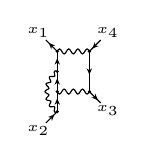
\begin{tikzpicture}[x=0.340cm, y=0.340cm, line width=0.420pt, baseline={([yshift=-0.6ex]0,0)}]
  \draw (-0.400,0.250) -- (-0.400,1.000);
  \fill (-0.400,0.744) -- (-0.502,0.506) -- (-0.400,0.583) -- (-0.298,0.506) -- cycle;
  \draw (0.800,1.000) -- (0.800,-0.500);
  \fill (0.800,0.131) -- (0.902,0.369) -- (0.800,0.292) -- (0.698,0.369) -- cycle;
  \draw (-0.400,-1.250) -- (-0.400,-0.500);
  \fill (-0.400,-0.756) -- (-0.502,-0.994) -- (-0.400,-0.917) -- (-0.298,-0.994) -- cycle;
  \draw (-0.400,-0.500) -- (-0.400,0.250);
  \fill (-0.400,-0.006) -- (-0.502,-0.244) -- (-0.400,-0.167) -- (-0.298,-0.244) -- cycle;
  \draw plot[smooth, tension=0.7] coordinates {(-0.400,1.000) (-0.357,1.065) (-0.314,1.093) (-0.271,1.065) (-0.229,1.000) (-0.186,0.935) (-0.143,0.907) (-0.100,0.935) (-0.057,1.000) (-0.014,1.065) (0.029,1.093) (0.071,1.065) (0.114,1.000) (0.157,0.935) (0.200,0.907) (0.243,0.935) (0.286,1.000) (0.329,1.065) (0.371,1.093) (0.414,1.065) (0.457,1.000) (0.500,0.935) (0.543,0.907) (0.586,0.935) (0.629,1.000) (0.671,1.065) (0.714,1.093) (0.757,1.065) (0.800,1.000)};
  \draw plot[smooth, tension=0.7] coordinates {(-0.400,-1.250) (-0.457,-1.270) (-0.498,-1.264) (-0.512,-1.225) (-0.505,-1.165) (-0.493,-1.106) (-0.500,-1.069) (-0.536,-1.059) (-0.595,-1.065) (-0.656,-1.067) (-0.693,-1.049) (-0.696,-1.008) (-0.671,-0.952) (-0.643,-0.900) (-0.638,-0.862) (-0.670,-0.842) (-0.728,-0.830) (-0.787,-0.815) (-0.818,-0.787) (-0.808,-0.747) (-0.768,-0.701) (-0.726,-0.659) (-0.711,-0.624) (-0.735,-0.596) (-0.788,-0.568) (-0.839,-0.536) (-0.860,-0.500) (-0.839,-0.464) (-0.788,-0.432) (-0.735,-0.404) (-0.711,-0.376) (-0.726,-0.341) (-0.768,-0.299) (-0.808,-0.253) (-0.818,-0.213) (-0.787,-0.185) (-0.728,-0.170) (-0.670,-0.158) (-0.638,-0.138) (-0.643,-0.100) (-0.671,-0.048) (-0.696,0.008) (-0.693,0.049) (-0.656,0.067) (-0.595,0.065) (-0.536,0.059) (-0.500,0.069) (-0.493,0.106) (-0.505,0.165) (-0.512,0.225) (-0.498,0.264) (-0.457,0.270) (-0.400,0.250)};
  \draw plot[smooth, tension=0.7] coordinates {(0.800,-0.500) (0.757,-0.565) (0.714,-0.593) (0.671,-0.565) (0.629,-0.500) (0.586,-0.435) (0.543,-0.407) (0.500,-0.435) (0.457,-0.500) (0.414,-0.565) (0.371,-0.593) (0.329,-0.565) (0.286,-0.500) (0.243,-0.435) (0.200,-0.407) (0.157,-0.435) (0.114,-0.500) (0.071,-0.565) (0.029,-0.593) (-0.014,-0.565) (-0.057,-0.500) (-0.100,-0.435) (-0.143,-0.407) (-0.186,-0.435) (-0.229,-0.500) (-0.271,-0.565) (-0.314,-0.593) (-0.357,-0.565) (-0.400,-0.500)};
  \draw (-0.400,1.000) -- (-0.824,1.424);
  \fill (-0.718,1.318) -- (-0.621,1.077) -- (-0.604,1.204) -- (-0.477,1.221) -- cycle;
  \draw (-0.400,-1.250) -- (-0.824,-1.674);
  \fill (-0.506,-1.356) -- (-0.747,-1.453) -- (-0.620,-1.470) -- (-0.603,-1.597) -- cycle;
  \draw (0.800,-0.500) -- (1.224,-0.924);
  \fill (1.118,-0.818) -- (1.021,-0.577) -- (1.004,-0.704) -- (0.877,-0.721) -- cycle;
  \draw (0.800,1.000) -- (1.224,1.424);
  \fill (0.906,1.106) -- (1.147,1.203) -- (1.020,1.220) -- (1.003,1.347) -- cycle;
  \fill (-0.400,1.000) circle (0.064);
  \fill (-0.400,-1.250) circle (0.064);
  \fill (0.800,-0.500) circle (0.064);
  \fill (0.800,1.000) circle (0.064);
  \fill (-0.400,-0.500) circle (0.064);
  \fill (-0.400,0.250) circle (0.064);
  \node[font=\tiny, inner sep=0pt, anchor=315] at (-0.888,1.488) {$x_{1}$};
  \node[font=\tiny, inner sep=0pt, anchor=45] at (-0.888,-1.738) {$x_{2}$};
  \node[font=\tiny, inner sep=0pt, anchor=135] at (1.288,-0.988) {$x_{3}$};
  \node[font=\tiny, inner sep=0pt, anchor=225] at (1.288,1.488) {$x_{4}$};
\end{tikzpicture}}
\diagramgap
\mbox{$\displaystyle +\,$\,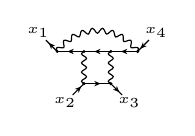
\begin{tikzpicture}[x=0.340cm, y=0.340cm, line width=0.420pt, baseline={([yshift=-0.6ex]0,0)}]
  \draw (-0.500,0.400) -- (-1.500,0.400);
  \fill (-1.119,0.400) -- (-0.881,0.298) -- (-0.958,0.400) -- (-0.881,0.502) -- cycle;
  \draw (-0.500,-0.800) -- (0.500,-0.800);
  \fill (0.119,-0.800) -- (-0.119,-0.698) -- (-0.042,-0.800) -- (-0.119,-0.902) -- cycle;
  \draw (1.500,0.400) -- (0.500,0.400);
  \fill (0.881,0.400) -- (1.119,0.298) -- (1.042,0.400) -- (1.119,0.502) -- cycle;
  \draw (0.500,0.400) -- (-0.500,0.400);
  \fill (-0.119,0.400) -- (0.119,0.298) -- (0.042,0.400) -- (0.119,0.502) -- cycle;
  \draw plot[smooth, tension=0.7] coordinates {(-1.500,0.400) (-1.528,0.478) (-1.521,0.533) (-1.469,0.554) (-1.386,0.546) (-1.305,0.535) (-1.255,0.548) (-1.244,0.599) (-1.259,0.679) (-1.270,0.761) (-1.252,0.814) (-1.197,0.824) (-1.118,0.799) (-1.041,0.772) (-0.988,0.775) (-0.968,0.823) (-0.966,0.905) (-0.961,0.987) (-0.933,1.036) (-0.877,1.034) (-0.804,0.994) (-0.734,0.952) (-0.682,0.944) (-0.652,0.987) (-0.634,1.067) (-0.612,1.147) (-0.575,1.188) (-0.521,1.175) (-0.458,1.122) (-0.397,1.067) (-0.348,1.049) (-0.310,1.085) (-0.276,1.159) (-0.239,1.233) (-0.194,1.266) (-0.144,1.243) (-0.092,1.178) (-0.045,1.111) (0.000,1.084) (0.045,1.111) (0.092,1.178) (0.144,1.243) (0.194,1.266) (0.239,1.233) (0.276,1.159) (0.310,1.085) (0.348,1.049) (0.397,1.067) (0.458,1.122) (0.521,1.175) (0.575,1.188) (0.612,1.147) (0.634,1.067) (0.652,0.987) (0.682,0.944) (0.734,0.952) (0.804,0.994) (0.877,1.034) (0.933,1.036) (0.961,0.987) (0.966,0.905) (0.968,0.823) (0.988,0.775) (1.041,0.772) (1.118,0.799) (1.197,0.824) (1.252,0.814) (1.270,0.761) (1.259,0.679) (1.244,0.599) (1.255,0.548) (1.305,0.535) (1.386,0.546) (1.469,0.554) (1.521,0.533) (1.528,0.478) (1.500,0.400)};
  \draw plot[smooth, tension=0.7] coordinates {(-0.500,-0.800) (-0.565,-0.757) (-0.593,-0.714) (-0.565,-0.671) (-0.500,-0.629) (-0.435,-0.586) (-0.407,-0.543) (-0.435,-0.500) (-0.500,-0.457) (-0.565,-0.414) (-0.593,-0.371) (-0.565,-0.329) (-0.500,-0.286) (-0.435,-0.243) (-0.407,-0.200) (-0.435,-0.157) (-0.500,-0.114) (-0.565,-0.071) (-0.593,-0.029) (-0.565,0.014) (-0.500,0.057) (-0.435,0.100) (-0.407,0.143) (-0.435,0.186) (-0.500,0.229) (-0.565,0.271) (-0.593,0.314) (-0.565,0.357) (-0.500,0.400)};
  \draw plot[smooth, tension=0.7] coordinates {(0.500,-0.800) (0.435,-0.757) (0.407,-0.714) (0.435,-0.671) (0.500,-0.629) (0.565,-0.586) (0.593,-0.543) (0.565,-0.500) (0.500,-0.457) (0.435,-0.414) (0.407,-0.371) (0.435,-0.329) (0.500,-0.286) (0.565,-0.243) (0.593,-0.200) (0.565,-0.157) (0.500,-0.114) (0.435,-0.071) (0.407,-0.029) (0.435,0.014) (0.500,0.057) (0.565,0.100) (0.593,0.143) (0.565,0.186) (0.500,0.229) (0.435,0.271) (0.407,0.314) (0.435,0.357) (0.500,0.400)};
  \draw (-1.500,0.400) -- (-1.924,0.824);
  \fill (-1.818,0.718) -- (-1.721,0.477) -- (-1.704,0.604) -- (-1.577,0.621) -- cycle;
  \draw (-0.500,-0.800) -- (-0.924,-1.224);
  \fill (-0.606,-0.906) -- (-0.847,-1.003) -- (-0.720,-1.020) -- (-0.703,-1.147) -- cycle;
  \draw (0.500,-0.800) -- (0.924,-1.224);
  \fill (0.818,-1.118) -- (0.721,-0.877) -- (0.704,-1.004) -- (0.577,-1.021) -- cycle;
  \draw (1.500,0.400) -- (1.924,0.824);
  \fill (1.606,0.506) -- (1.847,0.603) -- (1.720,0.620) -- (1.703,0.747) -- cycle;
  \fill (-1.500,0.400) circle (0.064);
  \fill (-0.500,-0.800) circle (0.064);
  \fill (0.500,-0.800) circle (0.064);
  \fill (1.500,0.400) circle (0.064);
  \fill (0.500,0.400) circle (0.064);
  \fill (-0.500,0.400) circle (0.064);
  \node[font=\tiny, inner sep=0pt, anchor=315] at (-1.988,0.888) {$x_{1}$};
  \node[font=\tiny, inner sep=0pt, anchor=45] at (-0.988,-1.288) {$x_{2}$};
  \node[font=\tiny, inner sep=0pt, anchor=135] at (0.988,-1.288) {$x_{3}$};
  \node[font=\tiny, inner sep=0pt, anchor=225] at (1.988,0.888) {$x_{4}$};
\end{tikzpicture}}
\diagramgap
\mbox{$\displaystyle -\,$\,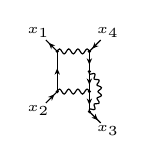
\begin{tikzpicture}[x=0.340cm, y=0.340cm, line width=0.420pt, baseline={([yshift=-0.6ex]0,0)}]
  \draw (-0.800,-0.500) -- (-0.800,1.000);
  \fill (-0.800,0.369) -- (-0.902,0.131) -- (-0.800,0.208) -- (-0.698,0.131) -- cycle;
  \draw (0.400,-0.500) -- (0.400,-1.250);
  \fill (0.400,-0.994) -- (0.502,-0.756) -- (0.400,-0.833) -- (0.298,-0.756) -- cycle;
  \draw (0.400,1.000) -- (0.400,0.250);
  \fill (0.400,0.506) -- (0.502,0.744) -- (0.400,0.667) -- (0.298,0.744) -- cycle;
  \draw (0.400,0.250) -- (0.400,-0.500);
  \fill (0.400,-0.244) -- (0.502,-0.006) -- (0.400,-0.083) -- (0.298,-0.006) -- cycle;
  \draw plot[smooth, tension=0.7] coordinates {(-0.800,1.000) (-0.757,1.065) (-0.714,1.093) (-0.671,1.065) (-0.629,1.000) (-0.586,0.935) (-0.543,0.907) (-0.500,0.935) (-0.457,1.000) (-0.414,1.065) (-0.371,1.093) (-0.329,1.065) (-0.286,1.000) (-0.243,0.935) (-0.200,0.907) (-0.157,0.935) (-0.114,1.000) (-0.071,1.065) (-0.029,1.093) (0.014,1.065) (0.057,1.000) (0.100,0.935) (0.143,0.907) (0.186,0.935) (0.229,1.000) (0.271,1.065) (0.314,1.093) (0.357,1.065) (0.400,1.000)};
  \draw plot[smooth, tension=0.7] coordinates {(-0.800,-0.500) (-0.757,-0.435) (-0.714,-0.407) (-0.671,-0.435) (-0.629,-0.500) (-0.586,-0.565) (-0.543,-0.593) (-0.500,-0.565) (-0.457,-0.500) (-0.414,-0.435) (-0.371,-0.407) (-0.329,-0.435) (-0.286,-0.500) (-0.243,-0.565) (-0.200,-0.593) (-0.157,-0.565) (-0.114,-0.500) (-0.071,-0.435) (-0.029,-0.407) (0.014,-0.435) (0.057,-0.500) (0.100,-0.565) (0.143,-0.593) (0.186,-0.565) (0.229,-0.500) (0.271,-0.435) (0.314,-0.407) (0.357,-0.435) (0.400,-0.500)};
  \draw plot[smooth, tension=0.7] coordinates {(0.400,-1.250) (0.397,-1.190) (0.409,-1.155) (0.447,-1.150) (0.505,-1.165) (0.564,-1.176) (0.604,-1.163) (0.612,-1.123) (0.595,-1.065) (0.575,-1.008) (0.577,-0.971) (0.611,-0.955) (0.671,-0.952) (0.731,-0.946) (0.765,-0.923) (0.761,-0.881) (0.728,-0.830) (0.693,-0.782) (0.683,-0.746) (0.712,-0.721) (0.768,-0.701) (0.823,-0.677) (0.850,-0.645) (0.834,-0.607) (0.788,-0.568) (0.740,-0.532) (0.720,-0.500) (0.740,-0.468) (0.788,-0.432) (0.834,-0.393) (0.850,-0.355) (0.823,-0.323) (0.768,-0.299) (0.712,-0.279) (0.683,-0.254) (0.693,-0.218) (0.728,-0.170) (0.761,-0.119) (0.765,-0.077) (0.731,-0.054) (0.671,-0.048) (0.611,-0.045) (0.577,-0.029) (0.575,0.008) (0.595,0.065) (0.612,0.123) (0.604,0.163) (0.564,0.176) (0.505,0.165) (0.447,0.150) (0.409,0.155) (0.397,0.190) (0.400,0.250)};
  \draw (-0.800,1.000) -- (-1.224,1.424);
  \fill (-1.118,1.318) -- (-1.021,1.077) -- (-1.004,1.204) -- (-0.877,1.221) -- cycle;
  \draw (-0.800,-0.500) -- (-1.224,-0.924);
  \fill (-0.906,-0.606) -- (-1.147,-0.703) -- (-1.020,-0.720) -- (-1.003,-0.847) -- cycle;
  \draw (0.400,-1.250) -- (0.824,-1.674);
  \fill (0.718,-1.568) -- (0.621,-1.327) -- (0.604,-1.454) -- (0.477,-1.471) -- cycle;
  \draw (0.400,1.000) -- (0.824,1.424);
  \fill (0.506,1.106) -- (0.747,1.203) -- (0.620,1.220) -- (0.603,1.347) -- cycle;
  \fill (-0.800,1.000) circle (0.064);
  \fill (-0.800,-0.500) circle (0.064);
  \fill (0.400,-1.250) circle (0.064);
  \fill (0.400,1.000) circle (0.064);
  \fill (0.400,0.250) circle (0.064);
  \fill (0.400,-0.500) circle (0.064);
  \node[font=\tiny, inner sep=0pt, anchor=315] at (-1.288,1.488) {$x_{1}$};
  \node[font=\tiny, inner sep=0pt, anchor=45] at (-1.288,-0.988) {$x_{2}$};
  \node[font=\tiny, inner sep=0pt, anchor=135] at (0.888,-1.738) {$x_{3}$};
  \node[font=\tiny, inner sep=0pt, anchor=225] at (0.888,1.488) {$x_{4}$};
\end{tikzpicture}}
\diagramgap
\mbox{$\displaystyle +\,$\,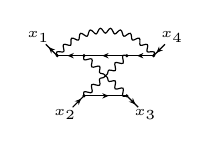
\begin{tikzpicture}[x=0.340cm, y=0.340cm, line width=0.420pt, baseline={([yshift=-0.6ex]0,0)}]
  \draw (-0.800,0.500) -- (-1.800,0.500);
  \fill (-1.419,0.500) -- (-1.181,0.398) -- (-1.258,0.500) -- (-1.181,0.602) -- cycle;
  \draw (-0.800,-1.000) -- (0.800,-1.000);
  \fill (0.119,-1.000) -- (-0.119,-0.898) -- (-0.042,-1.000) -- (-0.119,-1.102) -- cycle;
  \draw (1.800,0.500) -- (0.800,0.500);
  \fill (1.181,0.500) -- (1.419,0.398) -- (1.342,0.500) -- (1.419,0.602) -- cycle;
  \draw (0.800,0.500) -- (-0.800,0.500);
  \fill (-0.119,0.500) -- (0.119,0.398) -- (0.042,0.500) -- (0.119,0.602) -- cycle;
  \draw plot[smooth, tension=0.7] coordinates {(-1.800,0.500) (-1.828,0.577) (-1.822,0.632) (-1.770,0.652) (-1.689,0.646) (-1.608,0.636) (-1.558,0.651) (-1.548,0.702) (-1.565,0.781) (-1.580,0.862) (-1.565,0.915) (-1.511,0.926) (-1.431,0.906) (-1.353,0.884) (-1.302,0.890) (-1.284,0.939) (-1.287,1.020) (-1.288,1.102) (-1.264,1.151) (-1.209,1.154) (-1.134,1.121) (-1.061,1.086) (-1.009,1.083) (-0.983,1.128) (-0.974,1.209) (-0.961,1.290) (-0.929,1.335) (-0.874,1.328) (-0.806,1.283) (-0.740,1.236) (-0.689,1.225) (-0.656,1.265) (-0.633,1.343) (-0.607,1.421) (-0.568,1.460) (-0.515,1.444) (-0.455,1.388) (-0.398,1.331) (-0.349,1.311) (-0.310,1.346) (-0.274,1.419) (-0.236,1.491) (-0.191,1.523) (-0.142,1.499) (-0.092,1.434) (-0.044,1.368) (0.000,1.341) (0.044,1.368) (0.092,1.434) (0.142,1.499) (0.191,1.523) (0.236,1.491) (0.274,1.419) (0.310,1.346) (0.349,1.311) (0.398,1.331) (0.455,1.388) (0.515,1.444) (0.568,1.460) (0.607,1.421) (0.633,1.343) (0.656,1.265) (0.689,1.225) (0.740,1.236) (0.806,1.283) (0.874,1.328) (0.929,1.335) (0.961,1.290) (0.974,1.209) (0.983,1.128) (1.009,1.083) (1.061,1.086) (1.134,1.121) (1.209,1.154) (1.264,1.151) (1.288,1.102) (1.287,1.020) (1.284,0.939) (1.302,0.890) (1.353,0.884) (1.431,0.906) (1.511,0.926) (1.565,0.915) (1.580,0.862) (1.565,0.781) (1.548,0.702) (1.558,0.651) (1.608,0.636) (1.689,0.646) (1.770,0.652) (1.822,0.632) (1.828,0.577) (1.800,0.500)};
  \draw plot[smooth, tension=0.7] coordinates {(-0.800,-1.000) (-0.816,-0.910) (-0.801,-0.853) (-0.743,-0.842) (-0.655,-0.864) (-0.566,-0.885) (-0.508,-0.874) (-0.493,-0.817) (-0.509,-0.727) (-0.525,-0.638) (-0.510,-0.581) (-0.452,-0.569) (-0.364,-0.591) (-0.275,-0.612) (-0.217,-0.601) (-0.203,-0.544) (-0.218,-0.455) (-0.222,-0.377) (-0.188,-0.341) (-0.129,-0.331) (-0.073,-0.318) (-0.034,-0.287) (0.000,-0.250) (0.039,-0.219) (0.073,-0.182) (0.090,-0.127) (0.103,-0.068) (0.141,-0.036) (0.218,-0.045) (0.306,-0.067) (0.365,-0.056) (0.379,0.001) (0.364,0.091) (0.348,0.181) (0.363,0.238) (0.421,0.249) (0.509,0.227) (0.598,0.206) (0.655,0.217) (0.670,0.274) (0.655,0.364) (0.639,0.453) (0.654,0.510) (0.712,0.521) (0.800,0.500)};
  \draw plot[smooth, tension=0.7] coordinates {(0.800,-1.000) (0.712,-1.021) (0.654,-1.010) (0.639,-0.953) (0.655,-0.864) (0.670,-0.774) (0.655,-0.717) (0.598,-0.706) (0.509,-0.727) (0.421,-0.749) (0.363,-0.738) (0.348,-0.681) (0.364,-0.591) (0.379,-0.501) (0.365,-0.444) (0.306,-0.433) (0.218,-0.455) (0.141,-0.464) (0.103,-0.432) (0.090,-0.373) (0.073,-0.318) (0.039,-0.281) (0.000,-0.250) (-0.034,-0.213) (-0.073,-0.182) (-0.129,-0.169) (-0.188,-0.159) (-0.222,-0.123) (-0.218,-0.045) (-0.203,0.044) (-0.217,0.101) (-0.275,0.112) (-0.364,0.091) (-0.452,0.069) (-0.510,0.081) (-0.525,0.138) (-0.509,0.227) (-0.493,0.317) (-0.508,0.374) (-0.566,0.385) (-0.655,0.364) (-0.743,0.342) (-0.801,0.353) (-0.816,0.410) (-0.800,0.500)};
  \draw (-1.800,0.500) -- (-2.224,0.924);
  \fill (-2.118,0.818) -- (-2.021,0.577) -- (-2.004,0.704) -- (-1.877,0.721) -- cycle;
  \draw (-0.800,-1.000) -- (-1.224,-1.424);
  \fill (-0.906,-1.106) -- (-1.147,-1.203) -- (-1.020,-1.220) -- (-1.003,-1.347) -- cycle;
  \draw (0.800,-1.000) -- (1.224,-1.424);
  \fill (1.118,-1.318) -- (1.021,-1.077) -- (1.004,-1.204) -- (0.877,-1.221) -- cycle;
  \draw (1.800,0.500) -- (2.224,0.924);
  \fill (1.906,0.606) -- (2.147,0.703) -- (2.020,0.720) -- (2.003,0.847) -- cycle;
  \fill (-1.800,0.500) circle (0.064);
  \fill (-0.800,-1.000) circle (0.064);
  \fill (0.800,-1.000) circle (0.064);
  \fill (1.800,0.500) circle (0.064);
  \fill (0.800,0.500) circle (0.064);
  \fill (-0.800,0.500) circle (0.064);
  \node[font=\tiny, inner sep=0pt, anchor=315] at (-2.288,0.988) {$x_{1}$};
  \node[font=\tiny, inner sep=0pt, anchor=45] at (-1.288,-1.488) {$x_{2}$};
  \node[font=\tiny, inner sep=0pt, anchor=135] at (1.288,-1.488) {$x_{3}$};
  \node[font=\tiny, inner sep=0pt, anchor=225] at (2.288,0.988) {$x_{4}$};
\end{tikzpicture}}
\diagramgap
\mbox{$\displaystyle +\,$\,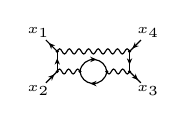
\begin{tikzpicture}[x=0.340cm, y=0.340cm, line width=0.420pt, baseline={([yshift=-0.6ex]0,0)}]
  \draw (-1.350,-0.250) -- (-1.350,0.500);
  \fill (-1.350,0.244) -- (-1.452,0.006) -- (-1.350,0.083) -- (-1.248,0.006) -- cycle;
  \draw (1.350,0.500) -- (1.350,-0.250);
  \fill (1.350,0.006) -- (1.452,0.244) -- (1.350,0.167) -- (1.248,0.244) -- cycle;
  \draw (0.500,-0.250) arc[start angle=353.974, end angle=186.026, radius=0.503];
  \fill (-0.119,-0.700) -- (0.119,-0.802) -- (0.042,-0.700) -- (0.119,-0.598) -- cycle;
  \draw (-0.500,-0.250) arc[start angle=173.974, end angle=6.026, radius=0.503];
  \fill (0.119,0.200) -- (-0.119,0.302) -- (-0.042,0.200) -- (-0.119,0.098) -- cycle;
  \draw plot[smooth, tension=0.7] coordinates {(-1.350,0.500) (-1.305,0.569) (-1.260,0.597) (-1.215,0.569) (-1.170,0.500) (-1.125,0.431) (-1.080,0.403) (-1.035,0.431) (-0.990,0.500) (-0.945,0.569) (-0.900,0.597) (-0.855,0.569) (-0.810,0.500) (-0.765,0.431) (-0.720,0.403) (-0.675,0.431) (-0.630,0.500) (-0.585,0.569) (-0.540,0.597) (-0.495,0.569) (-0.450,0.500) (-0.405,0.431) (-0.360,0.403) (-0.315,0.431) (-0.270,0.500) (-0.225,0.569) (-0.180,0.597) (-0.135,0.569) (-0.090,0.500) (-0.045,0.431) (0.000,0.403) (0.045,0.431) (0.090,0.500) (0.135,0.569) (0.180,0.597) (0.225,0.569) (0.270,0.500) (0.315,0.431) (0.360,0.403) (0.405,0.431) (0.450,0.500) (0.495,0.569) (0.540,0.597) (0.585,0.569) (0.630,0.500) (0.675,0.431) (0.720,0.403) (0.765,0.431) (0.810,0.500) (0.855,0.569) (0.900,0.597) (0.945,0.569) (0.990,0.500) (1.035,0.431) (1.080,0.403) (1.125,0.431) (1.170,0.500) (1.215,0.569) (1.260,0.597) (1.305,0.569) (1.350,0.500)};
  \draw plot[smooth, tension=0.7] coordinates {(-1.350,-0.250) (-1.308,-0.185) (-1.265,-0.158) (-1.223,-0.185) (-1.180,-0.250) (-1.138,-0.315) (-1.095,-0.342) (-1.052,-0.315) (-1.010,-0.250) (-0.968,-0.185) (-0.925,-0.158) (-0.883,-0.185) (-0.840,-0.250) (-0.798,-0.315) (-0.755,-0.342) (-0.713,-0.315) (-0.670,-0.250) (-0.628,-0.185) (-0.585,-0.158) (-0.543,-0.185) (-0.500,-0.250)};
  \draw plot[smooth, tension=0.7] coordinates {(1.350,-0.250) (1.308,-0.315) (1.265,-0.342) (1.223,-0.315) (1.180,-0.250) (1.138,-0.185) (1.095,-0.158) (1.052,-0.185) (1.010,-0.250) (0.968,-0.315) (0.925,-0.342) (0.883,-0.315) (0.840,-0.250) (0.798,-0.185) (0.755,-0.158) (0.712,-0.185) (0.670,-0.250) (0.628,-0.315) (0.585,-0.342) (0.542,-0.315) (0.500,-0.250)};
  \draw (-1.350,0.500) -- (-1.774,0.924);
  \fill (-1.668,0.818) -- (-1.571,0.577) -- (-1.554,0.704) -- (-1.427,0.721) -- cycle;
  \draw (-1.350,-0.250) -- (-1.774,-0.674);
  \fill (-1.456,-0.356) -- (-1.697,-0.453) -- (-1.570,-0.470) -- (-1.553,-0.597) -- cycle;
  \draw (1.350,-0.250) -- (1.774,-0.674);
  \fill (1.668,-0.568) -- (1.571,-0.327) -- (1.554,-0.454) -- (1.427,-0.471) -- cycle;
  \draw (1.350,0.500) -- (1.774,0.924);
  \fill (1.456,0.606) -- (1.697,0.703) -- (1.570,0.720) -- (1.553,0.847) -- cycle;
  \fill (-1.350,0.500) circle (0.064);
  \fill (-1.350,-0.250) circle (0.064);
  \fill (1.350,-0.250) circle (0.064);
  \fill (1.350,0.500) circle (0.064);
  \fill (-0.500,-0.250) circle (0.064);
  \fill (0.500,-0.250) circle (0.064);
  \node[font=\tiny, inner sep=0pt, anchor=315] at (-1.838,0.988) {$x_{1}$};
  \node[font=\tiny, inner sep=0pt, anchor=45] at (-1.838,-0.738) {$x_{2}$};
  \node[font=\tiny, inner sep=0pt, anchor=135] at (1.838,-0.738) {$x_{3}$};
  \node[font=\tiny, inner sep=0pt, anchor=225] at (1.838,0.988) {$x_{4}$};
\end{tikzpicture}}
\diagramgap
\mbox{$\displaystyle -\,$\,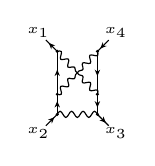
\begin{tikzpicture}[x=0.340cm, y=0.340cm, line width=0.420pt, baseline={([yshift=-0.6ex]0,0)}]
  \draw (-0.750,-0.283) -- (-0.750,1.317);
  \fill (-0.750,0.636) -- (-0.852,0.397) -- (-0.750,0.475) -- (-0.648,0.397) -- cycle;
  \draw (0.750,-0.283) -- (0.750,-1.033);
  \fill (0.750,-0.778) -- (0.852,-0.539) -- (0.750,-0.617) -- (0.648,-0.539) -- cycle;
  \draw (-0.750,-1.033) -- (-0.750,-0.283);
  \fill (-0.750,-0.539) -- (-0.852,-0.778) -- (-0.750,-0.700) -- (-0.648,-0.778) -- cycle;
  \draw (0.750,1.317) -- (0.750,-0.283);
  \fill (0.750,0.397) -- (0.852,0.636) -- (0.750,0.558) -- (0.648,0.636) -- cycle;
  \draw plot[smooth, tension=0.7] coordinates {(-0.750,1.317) (-0.660,1.332) (-0.603,1.318) (-0.592,1.260) (-0.614,1.171) (-0.635,1.083) (-0.624,1.025) (-0.567,1.010) (-0.477,1.026) (-0.388,1.041) (-0.331,1.027) (-0.319,0.969) (-0.341,0.880) (-0.362,0.792) (-0.351,0.734) (-0.294,0.719) (-0.205,0.735) (-0.127,0.739) (-0.091,0.705) (-0.081,0.645) (-0.068,0.589) (-0.037,0.550) (0.000,0.517) (0.031,0.478) (0.068,0.444) (0.123,0.427) (0.182,0.414) (0.214,0.375) (0.205,0.298) (0.183,0.210) (0.194,0.152) (0.251,0.137) (0.341,0.153) (0.431,0.169) (0.488,0.154) (0.499,0.096) (0.477,0.008) (0.456,-0.081) (0.467,-0.139) (0.524,-0.154) (0.614,-0.138) (0.703,-0.122) (0.760,-0.137) (0.771,-0.195) (0.750,-0.283)};
  \draw plot[smooth, tension=0.7] coordinates {(-0.750,-1.033) (-0.696,-0.952) (-0.643,-0.918) (-0.589,-0.952) (-0.536,-1.033) (-0.482,-1.115) (-0.429,-1.149) (-0.375,-1.115) (-0.321,-1.033) (-0.268,-0.952) (-0.214,-0.918) (-0.161,-0.952) (-0.107,-1.033) (-0.054,-1.115) (0.000,-1.149) (0.054,-1.115) (0.107,-1.033) (0.161,-0.952) (0.214,-0.918) (0.268,-0.952) (0.321,-1.033) (0.375,-1.115) (0.429,-1.149) (0.482,-1.115) (0.536,-1.033) (0.589,-0.952) (0.643,-0.918) (0.696,-0.952) (0.750,-1.033)};
  \draw plot[smooth, tension=0.7] coordinates {(0.750,1.317) (0.771,1.228) (0.760,1.170) (0.703,1.156) (0.614,1.171) (0.524,1.187) (0.467,1.172) (0.456,1.114) (0.477,1.026) (0.499,0.937) (0.488,0.879) (0.431,0.865) (0.341,0.880) (0.251,0.896) (0.194,0.881) (0.183,0.823) (0.205,0.735) (0.214,0.658) (0.182,0.619) (0.123,0.606) (0.068,0.589) (0.031,0.556) (0.000,0.517) (-0.037,0.483) (-0.068,0.444) (-0.081,0.388) (-0.091,0.328) (-0.127,0.294) (-0.205,0.298) (-0.294,0.314) (-0.351,0.299) (-0.362,0.241) (-0.341,0.153) (-0.319,0.065) (-0.331,0.007) (-0.388,-0.008) (-0.477,0.008) (-0.567,0.023) (-0.624,0.008) (-0.635,-0.049) (-0.614,-0.138) (-0.592,-0.226) (-0.603,-0.284) (-0.660,-0.299) (-0.750,-0.283)};
  \draw (-0.750,1.317) -- (-1.174,1.741);
  \fill (-1.068,1.634) -- (-0.971,1.393) -- (-0.954,1.520) -- (-0.827,1.538) -- cycle;
  \draw (-0.750,-1.033) -- (-1.174,-1.458);
  \fill (-0.856,-1.140) -- (-1.097,-1.237) -- (-0.970,-1.254) -- (-0.953,-1.381) -- cycle;
  \draw (0.750,-1.033) -- (1.174,-1.458);
  \fill (1.068,-1.351) -- (0.971,-1.110) -- (0.954,-1.237) -- (0.827,-1.254) -- cycle;
  \draw (0.750,1.317) -- (1.174,1.741);
  \fill (0.856,1.423) -- (1.097,1.520) -- (0.970,1.537) -- (0.953,1.664) -- cycle;
  \fill (-0.750,1.317) circle (0.064);
  \fill (-0.750,-1.033) circle (0.064);
  \fill (0.750,-1.033) circle (0.064);
  \fill (0.750,1.317) circle (0.064);
  \fill (-0.750,-0.283) circle (0.064);
  \fill (0.750,-0.283) circle (0.064);
  \node[font=\tiny, inner sep=0pt, anchor=315] at (-1.238,1.805) {$x_{1}$};
  \node[font=\tiny, inner sep=0pt, anchor=45] at (-1.238,-1.521) {$x_{2}$};
  \node[font=\tiny, inner sep=0pt, anchor=135] at (1.238,-1.521) {$x_{3}$};
  \node[font=\tiny, inner sep=0pt, anchor=225] at (1.238,1.805) {$x_{4}$};
\end{tikzpicture}}
\diagramgap
\mbox{$\displaystyle +\,$\,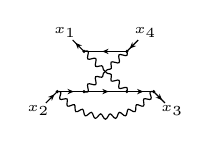
\begin{tikzpicture}[x=0.340cm, y=0.340cm, line width=0.420pt, baseline={([yshift=-0.6ex]0,0)}]
  \draw (0.800,1.000) -- (-0.800,1.000);
  \fill (-0.119,1.000) -- (0.119,0.898) -- (0.042,1.000) -- (0.119,1.102) -- cycle;
  \draw (0.800,-0.500) -- (1.800,-0.500);
  \fill (1.419,-0.500) -- (1.181,-0.398) -- (1.258,-0.500) -- (1.181,-0.602) -- cycle;
  \draw (-1.800,-0.500) -- (-0.800,-0.500);
  \fill (-1.181,-0.500) -- (-1.419,-0.398) -- (-1.342,-0.500) -- (-1.419,-0.602) -- cycle;
  \draw (-0.800,-0.500) -- (0.800,-0.500);
  \fill (0.119,-0.500) -- (-0.119,-0.398) -- (-0.042,-0.500) -- (-0.119,-0.602) -- cycle;
  \draw plot[smooth, tension=0.7] coordinates {(-0.800,1.000) (-0.712,1.021) (-0.654,1.010) (-0.639,0.953) (-0.655,0.864) (-0.670,0.774) (-0.655,0.717) (-0.598,0.706) (-0.509,0.727) (-0.421,0.749) (-0.363,0.738) (-0.348,0.681) (-0.364,0.591) (-0.379,0.501) (-0.365,0.444) (-0.306,0.433) (-0.218,0.455) (-0.141,0.464) (-0.103,0.432) (-0.090,0.373) (-0.073,0.318) (-0.039,0.281) (0.000,0.250) (0.034,0.213) (0.073,0.182) (0.129,0.169) (0.188,0.159) (0.222,0.123) (0.218,0.045) (0.203,-0.044) (0.217,-0.101) (0.275,-0.112) (0.364,-0.091) (0.452,-0.069) (0.510,-0.081) (0.525,-0.138) (0.509,-0.227) (0.493,-0.317) (0.508,-0.374) (0.566,-0.385) (0.655,-0.364) (0.743,-0.342) (0.801,-0.353) (0.816,-0.410) (0.800,-0.500)};
  \draw plot[smooth, tension=0.7] coordinates {(-1.800,-0.500) (-1.719,-0.497) (-1.670,-0.516) (-1.665,-0.568) (-1.689,-0.646) (-1.710,-0.725) (-1.699,-0.779) (-1.646,-0.795) (-1.565,-0.781) (-1.486,-0.765) (-1.435,-0.775) (-1.421,-0.826) (-1.431,-0.906) (-1.439,-0.988) (-1.419,-1.039) (-1.365,-1.046) (-1.287,-1.020) (-1.212,-0.991) (-1.159,-0.992) (-1.137,-1.040) (-1.134,-1.121) (-1.128,-1.203) (-1.101,-1.250) (-1.046,-1.248) (-0.974,-1.209) (-0.904,-1.168) (-0.852,-1.160) (-0.822,-1.204) (-0.806,-1.283) (-0.786,-1.363) (-0.751,-1.405) (-0.697,-1.394) (-0.633,-1.343) (-0.571,-1.291) (-0.521,-1.275) (-0.485,-1.313) (-0.455,-1.388) (-0.423,-1.464) (-0.381,-1.500) (-0.330,-1.479) (-0.274,-1.419) (-0.222,-1.357) (-0.175,-1.333) (-0.133,-1.364) (-0.092,-1.434) (-0.047,-1.503) (0.000,-1.531) (0.047,-1.503) (0.092,-1.434) (0.133,-1.364) (0.175,-1.333) (0.222,-1.357) (0.274,-1.419) (0.330,-1.479) (0.381,-1.500) (0.423,-1.464) (0.455,-1.388) (0.485,-1.313) (0.521,-1.275) (0.571,-1.291) (0.633,-1.343) (0.697,-1.394) (0.751,-1.405) (0.786,-1.363) (0.806,-1.283) (0.822,-1.204) (0.852,-1.160) (0.904,-1.168) (0.974,-1.209) (1.046,-1.248) (1.101,-1.250) (1.128,-1.203) (1.134,-1.121) (1.137,-1.040) (1.159,-0.992) (1.212,-0.991) (1.287,-1.020) (1.365,-1.046) (1.419,-1.039) (1.439,-0.988) (1.431,-0.906) (1.421,-0.826) (1.435,-0.775) (1.486,-0.765) (1.565,-0.781) (1.646,-0.795) (1.699,-0.779) (1.710,-0.725) (1.689,-0.646) (1.665,-0.568) (1.670,-0.516) (1.719,-0.497) (1.800,-0.500)};
  \draw plot[smooth, tension=0.7] coordinates {(0.800,1.000) (0.816,0.910) (0.801,0.853) (0.743,0.842) (0.655,0.864) (0.566,0.885) (0.508,0.874) (0.493,0.817) (0.509,0.727) (0.525,0.638) (0.510,0.581) (0.452,0.569) (0.364,0.591) (0.275,0.612) (0.217,0.601) (0.203,0.544) (0.218,0.455) (0.222,0.377) (0.188,0.341) (0.129,0.331) (0.073,0.318) (0.034,0.287) (0.000,0.250) (-0.039,0.219) (-0.073,0.182) (-0.090,0.127) (-0.103,0.068) (-0.141,0.036) (-0.218,0.045) (-0.306,0.067) (-0.365,0.056) (-0.379,-0.001) (-0.364,-0.091) (-0.348,-0.181) (-0.363,-0.238) (-0.421,-0.249) (-0.509,-0.227) (-0.598,-0.206) (-0.655,-0.217) (-0.670,-0.274) (-0.655,-0.364) (-0.639,-0.453) (-0.654,-0.510) (-0.712,-0.521) (-0.800,-0.500)};
  \draw (-0.800,1.000) -- (-1.224,1.424);
  \fill (-1.118,1.318) -- (-1.021,1.077) -- (-1.004,1.204) -- (-0.877,1.221) -- cycle;
  \draw (-1.800,-0.500) -- (-2.224,-0.924);
  \fill (-1.906,-0.606) -- (-2.147,-0.703) -- (-2.020,-0.720) -- (-2.003,-0.847) -- cycle;
  \draw (1.800,-0.500) -- (2.224,-0.924);
  \fill (2.118,-0.818) -- (2.021,-0.577) -- (2.004,-0.704) -- (1.877,-0.721) -- cycle;
  \draw (0.800,1.000) -- (1.224,1.424);
  \fill (0.906,1.106) -- (1.147,1.203) -- (1.020,1.220) -- (1.003,1.347) -- cycle;
  \fill (-0.800,1.000) circle (0.064);
  \fill (-1.800,-0.500) circle (0.064);
  \fill (1.800,-0.500) circle (0.064);
  \fill (0.800,1.000) circle (0.064);
  \fill (-0.800,-0.500) circle (0.064);
  \fill (0.800,-0.500) circle (0.064);
  \node[font=\tiny, inner sep=0pt, anchor=315] at (-1.288,1.488) {$x_{1}$};
  \node[font=\tiny, inner sep=0pt, anchor=45] at (-2.288,-0.988) {$x_{2}$};
  \node[font=\tiny, inner sep=0pt, anchor=135] at (2.288,-0.988) {$x_{3}$};
  \node[font=\tiny, inner sep=0pt, anchor=225] at (1.288,1.488) {$x_{4}$};
\end{tikzpicture}}
\diagramgap
\mbox{$\displaystyle -\,$\,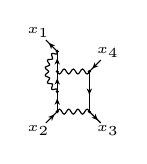
\begin{tikzpicture}[x=0.340cm, y=0.340cm, line width=0.420pt, baseline={([yshift=-0.6ex]0,0)}]
  \draw (-0.400,0.500) -- (-0.400,1.250);
  \fill (-0.400,0.994) -- (-0.502,0.756) -- (-0.400,0.833) -- (-0.298,0.756) -- cycle;
  \draw (0.800,0.500) -- (0.800,-1.000);
  \fill (0.800,-0.369) -- (0.902,-0.131) -- (0.800,-0.208) -- (0.698,-0.131) -- cycle;
  \draw (-0.400,-1.000) -- (-0.400,-0.250);
  \fill (-0.400,-0.506) -- (-0.502,-0.744) -- (-0.400,-0.667) -- (-0.298,-0.744) -- cycle;
  \draw (-0.400,-0.250) -- (-0.400,0.500);
  \fill (-0.400,0.244) -- (-0.502,0.006) -- (-0.400,0.083) -- (-0.298,0.006) -- cycle;
  \draw plot[smooth, tension=0.7] coordinates {(-0.400,1.250) (-0.397,1.190) (-0.409,1.155) (-0.447,1.150) (-0.505,1.165) (-0.564,1.176) (-0.604,1.163) (-0.612,1.123) (-0.595,1.065) (-0.575,1.008) (-0.577,0.971) (-0.611,0.955) (-0.671,0.952) (-0.731,0.946) (-0.765,0.923) (-0.761,0.881) (-0.728,0.830) (-0.693,0.782) (-0.683,0.746) (-0.712,0.721) (-0.768,0.701) (-0.823,0.677) (-0.850,0.645) (-0.834,0.607) (-0.788,0.568) (-0.740,0.532) (-0.720,0.500) (-0.740,0.468) (-0.788,0.432) (-0.834,0.393) (-0.850,0.355) (-0.823,0.323) (-0.768,0.299) (-0.712,0.279) (-0.683,0.254) (-0.693,0.218) (-0.728,0.170) (-0.761,0.119) (-0.765,0.077) (-0.731,0.054) (-0.671,0.048) (-0.611,0.045) (-0.577,0.029) (-0.575,-0.008) (-0.595,-0.065) (-0.612,-0.123) (-0.604,-0.163) (-0.564,-0.176) (-0.505,-0.165) (-0.447,-0.150) (-0.409,-0.155) (-0.397,-0.190) (-0.400,-0.250)};
  \draw plot[smooth, tension=0.7] coordinates {(-0.400,-1.000) (-0.357,-0.935) (-0.314,-0.907) (-0.271,-0.935) (-0.229,-1.000) (-0.186,-1.065) (-0.143,-1.093) (-0.100,-1.065) (-0.057,-1.000) (-0.014,-0.935) (0.029,-0.907) (0.071,-0.935) (0.114,-1.000) (0.157,-1.065) (0.200,-1.093) (0.243,-1.065) (0.286,-1.000) (0.329,-0.935) (0.371,-0.907) (0.414,-0.935) (0.457,-1.000) (0.500,-1.065) (0.543,-1.093) (0.586,-1.065) (0.629,-1.000) (0.671,-0.935) (0.714,-0.907) (0.757,-0.935) (0.800,-1.000)};
  \draw plot[smooth, tension=0.7] coordinates {(0.800,0.500) (0.757,0.435) (0.714,0.407) (0.671,0.435) (0.629,0.500) (0.586,0.565) (0.543,0.593) (0.500,0.565) (0.457,0.500) (0.414,0.435) (0.371,0.407) (0.329,0.435) (0.286,0.500) (0.243,0.565) (0.200,0.593) (0.157,0.565) (0.114,0.500) (0.071,0.435) (0.029,0.407) (-0.014,0.435) (-0.057,0.500) (-0.100,0.565) (-0.143,0.593) (-0.186,0.565) (-0.229,0.500) (-0.271,0.435) (-0.314,0.407) (-0.357,0.435) (-0.400,0.500)};
  \draw (-0.400,1.250) -- (-0.824,1.674);
  \fill (-0.718,1.568) -- (-0.621,1.327) -- (-0.604,1.454) -- (-0.477,1.471) -- cycle;
  \draw (-0.400,-1.000) -- (-0.824,-1.424);
  \fill (-0.506,-1.106) -- (-0.747,-1.203) -- (-0.620,-1.220) -- (-0.603,-1.347) -- cycle;
  \draw (0.800,-1.000) -- (1.224,-1.424);
  \fill (1.118,-1.318) -- (1.021,-1.077) -- (1.004,-1.204) -- (0.877,-1.221) -- cycle;
  \draw (0.800,0.500) -- (1.224,0.924);
  \fill (0.906,0.606) -- (1.147,0.703) -- (1.020,0.720) -- (1.003,0.847) -- cycle;
  \fill (-0.400,1.250) circle (0.064);
  \fill (-0.400,-1.000) circle (0.064);
  \fill (0.800,-1.000) circle (0.064);
  \fill (0.800,0.500) circle (0.064);
  \fill (-0.400,-0.250) circle (0.064);
  \fill (-0.400,0.500) circle (0.064);
  \node[font=\tiny, inner sep=0pt, anchor=315] at (-0.888,1.738) {$x_{1}$};
  \node[font=\tiny, inner sep=0pt, anchor=45] at (-0.888,-1.488) {$x_{2}$};
  \node[font=\tiny, inner sep=0pt, anchor=135] at (1.288,-1.488) {$x_{3}$};
  \node[font=\tiny, inner sep=0pt, anchor=225] at (1.288,0.988) {$x_{4}$};
\end{tikzpicture}}
\diagramgap
\mbox{$\displaystyle +\,$\,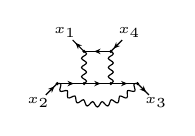
\begin{tikzpicture}[x=0.340cm, y=0.340cm, line width=0.420pt, baseline={([yshift=-0.6ex]0,0)}]
  \draw (0.500,0.800) -- (-0.500,0.800);
  \fill (-0.119,0.800) -- (0.119,0.698) -- (0.042,0.800) -- (0.119,0.902) -- cycle;
  \draw (0.500,-0.400) -- (1.500,-0.400);
  \fill (1.119,-0.400) -- (0.881,-0.298) -- (0.958,-0.400) -- (0.881,-0.502) -- cycle;
  \draw (-1.500,-0.400) -- (-0.500,-0.400);
  \fill (-0.881,-0.400) -- (-1.119,-0.298) -- (-1.042,-0.400) -- (-1.119,-0.502) -- cycle;
  \draw (-0.500,-0.400) -- (0.500,-0.400);
  \fill (0.119,-0.400) -- (-0.119,-0.298) -- (-0.042,-0.400) -- (-0.119,-0.502) -- cycle;
  \draw plot[smooth, tension=0.7] coordinates {(-0.500,0.800) (-0.435,0.757) (-0.407,0.714) (-0.435,0.671) (-0.500,0.629) (-0.565,0.586) (-0.593,0.543) (-0.565,0.500) (-0.500,0.457) (-0.435,0.414) (-0.407,0.371) (-0.435,0.329) (-0.500,0.286) (-0.565,0.243) (-0.593,0.200) (-0.565,0.157) (-0.500,0.114) (-0.435,0.071) (-0.407,0.029) (-0.435,-0.014) (-0.500,-0.057) (-0.565,-0.100) (-0.593,-0.143) (-0.565,-0.186) (-0.500,-0.229) (-0.435,-0.271) (-0.407,-0.314) (-0.435,-0.357) (-0.500,-0.400)};
  \draw plot[smooth, tension=0.7] coordinates {(-1.500,-0.400) (-1.418,-0.397) (-1.369,-0.415) (-1.364,-0.467) (-1.386,-0.546) (-1.406,-0.626) (-1.394,-0.681) (-1.340,-0.695) (-1.259,-0.679) (-1.179,-0.660) (-1.127,-0.668) (-1.111,-0.718) (-1.118,-0.799) (-1.121,-0.882) (-1.098,-0.933) (-1.042,-0.937) (-0.966,-0.905) (-0.892,-0.870) (-0.840,-0.867) (-0.814,-0.913) (-0.804,-0.994) (-0.791,-1.076) (-0.758,-1.121) (-0.702,-1.113) (-0.634,-1.067) (-0.569,-1.018) (-0.518,-1.005) (-0.484,-1.044) (-0.458,-1.122) (-0.428,-1.199) (-0.387,-1.237) (-0.334,-1.218) (-0.276,-1.159) (-0.222,-1.098) (-0.175,-1.075) (-0.133,-1.107) (-0.092,-1.178) (-0.048,-1.247) (0.000,-1.276) (0.048,-1.247) (0.092,-1.178) (0.133,-1.107) (0.175,-1.075) (0.222,-1.098) (0.276,-1.159) (0.334,-1.218) (0.387,-1.237) (0.428,-1.199) (0.458,-1.122) (0.484,-1.044) (0.518,-1.005) (0.569,-1.018) (0.634,-1.067) (0.702,-1.113) (0.758,-1.121) (0.791,-1.076) (0.804,-0.994) (0.814,-0.913) (0.840,-0.867) (0.892,-0.870) (0.966,-0.905) (1.042,-0.937) (1.098,-0.933) (1.121,-0.882) (1.118,-0.799) (1.111,-0.718) (1.127,-0.668) (1.179,-0.660) (1.259,-0.679) (1.340,-0.695) (1.394,-0.681) (1.406,-0.626) (1.386,-0.546) (1.364,-0.467) (1.369,-0.415) (1.418,-0.397) (1.500,-0.400)};
  \draw plot[smooth, tension=0.7] coordinates {(0.500,0.800) (0.565,0.757) (0.593,0.714) (0.565,0.671) (0.500,0.629) (0.435,0.586) (0.407,0.543) (0.435,0.500) (0.500,0.457) (0.565,0.414) (0.593,0.371) (0.565,0.329) (0.500,0.286) (0.435,0.243) (0.407,0.200) (0.435,0.157) (0.500,0.114) (0.565,0.071) (0.593,0.029) (0.565,-0.014) (0.500,-0.057) (0.435,-0.100) (0.407,-0.143) (0.435,-0.186) (0.500,-0.229) (0.565,-0.271) (0.593,-0.314) (0.565,-0.357) (0.500,-0.400)};
  \draw (-0.500,0.800) -- (-0.924,1.224);
  \fill (-0.818,1.118) -- (-0.721,0.877) -- (-0.704,1.004) -- (-0.577,1.021) -- cycle;
  \draw (-1.500,-0.400) -- (-1.924,-0.824);
  \fill (-1.606,-0.506) -- (-1.847,-0.603) -- (-1.720,-0.620) -- (-1.703,-0.747) -- cycle;
  \draw (1.500,-0.400) -- (1.924,-0.824);
  \fill (1.818,-0.718) -- (1.721,-0.477) -- (1.704,-0.604) -- (1.577,-0.621) -- cycle;
  \draw (0.500,0.800) -- (0.924,1.224);
  \fill (0.606,0.906) -- (0.847,1.003) -- (0.720,1.020) -- (0.703,1.147) -- cycle;
  \fill (-0.500,0.800) circle (0.064);
  \fill (-1.500,-0.400) circle (0.064);
  \fill (1.500,-0.400) circle (0.064);
  \fill (0.500,0.800) circle (0.064);
  \fill (-0.500,-0.400) circle (0.064);
  \fill (0.500,-0.400) circle (0.064);
  \node[font=\tiny, inner sep=0pt, anchor=315] at (-0.988,1.288) {$x_{1}$};
  \node[font=\tiny, inner sep=0pt, anchor=45] at (-1.988,-0.888) {$x_{2}$};
  \node[font=\tiny, inner sep=0pt, anchor=135] at (1.988,-0.888) {$x_{3}$};
  \node[font=\tiny, inner sep=0pt, anchor=225] at (0.988,1.288) {$x_{4}$};
\end{tikzpicture}}
\diagramgap
\mbox{$\displaystyle -\,$\,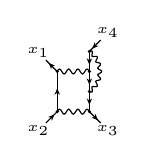
\begin{tikzpicture}[x=0.340cm, y=0.340cm, line width=0.420pt, baseline={([yshift=-0.6ex]0,0)}]
  \draw (-0.800,-1.000) -- (-0.800,0.500);
  \fill (-0.800,-0.131) -- (-0.902,-0.369) -- (-0.800,-0.292) -- (-0.698,-0.369) -- cycle;
  \draw (0.400,-0.250) -- (0.400,-1.000);
  \fill (0.400,-0.744) -- (0.502,-0.506) -- (0.400,-0.583) -- (0.298,-0.506) -- cycle;
  \draw (0.400,1.250) -- (0.400,0.500);
  \fill (0.400,0.756) -- (0.502,0.994) -- (0.400,0.917) -- (0.298,0.994) -- cycle;
  \draw (0.400,0.500) -- (0.400,-0.250);
  \fill (0.400,0.006) -- (0.502,0.244) -- (0.400,0.167) -- (0.298,0.244) -- cycle;
  \draw plot[smooth, tension=0.7] coordinates {(-0.800,0.500) (-0.757,0.565) (-0.714,0.593) (-0.671,0.565) (-0.629,0.500) (-0.586,0.435) (-0.543,0.407) (-0.500,0.435) (-0.457,0.500) (-0.414,0.565) (-0.371,0.593) (-0.329,0.565) (-0.286,0.500) (-0.243,0.435) (-0.200,0.407) (-0.157,0.435) (-0.114,0.500) (-0.071,0.565) (-0.029,0.593) (0.014,0.565) (0.057,0.500) (0.100,0.435) (0.143,0.407) (0.186,0.435) (0.229,0.500) (0.271,0.565) (0.314,0.593) (0.357,0.565) (0.400,0.500)};
  \draw plot[smooth, tension=0.7] coordinates {(-0.800,-1.000) (-0.757,-0.935) (-0.714,-0.907) (-0.671,-0.935) (-0.629,-1.000) (-0.586,-1.065) (-0.543,-1.093) (-0.500,-1.065) (-0.457,-1.000) (-0.414,-0.935) (-0.371,-0.907) (-0.329,-0.935) (-0.286,-1.000) (-0.243,-1.065) (-0.200,-1.093) (-0.157,-1.065) (-0.114,-1.000) (-0.071,-0.935) (-0.029,-0.907) (0.014,-0.935) (0.057,-1.000) (0.100,-1.065) (0.143,-1.093) (0.186,-1.065) (0.229,-1.000) (0.271,-0.935) (0.314,-0.907) (0.357,-0.935) (0.400,-1.000)};
  \draw plot[smooth, tension=0.7] coordinates {(0.400,1.250) (0.457,1.270) (0.498,1.264) (0.512,1.225) (0.505,1.165) (0.493,1.106) (0.500,1.069) (0.536,1.059) (0.595,1.065) (0.656,1.067) (0.693,1.049) (0.696,1.008) (0.671,0.952) (0.643,0.900) (0.638,0.862) (0.670,0.842) (0.728,0.830) (0.787,0.815) (0.818,0.787) (0.808,0.747) (0.768,0.701) (0.726,0.659) (0.711,0.624) (0.735,0.596) (0.788,0.568) (0.839,0.536) (0.860,0.500) (0.839,0.464) (0.788,0.432) (0.735,0.404) (0.711,0.376) (0.726,0.341) (0.768,0.299) (0.808,0.253) (0.818,0.213) (0.787,0.185) (0.728,0.170) (0.670,0.158) (0.638,0.138) (0.643,0.100) (0.671,0.048) (0.696,-0.008) (0.693,-0.049) (0.656,-0.067) (0.595,-0.065) (0.536,-0.059) (0.500,-0.069) (0.493,-0.106) (0.505,-0.165) (0.512,-0.225) (0.498,-0.264) (0.457,-0.270) (0.400,-0.250)};
  \draw (-0.800,0.500) -- (-1.224,0.924);
  \fill (-1.118,0.818) -- (-1.021,0.577) -- (-1.004,0.704) -- (-0.877,0.721) -- cycle;
  \draw (-0.800,-1.000) -- (-1.224,-1.424);
  \fill (-0.906,-1.106) -- (-1.147,-1.203) -- (-1.020,-1.220) -- (-1.003,-1.347) -- cycle;
  \draw (0.400,-1.000) -- (0.824,-1.424);
  \fill (0.718,-1.318) -- (0.621,-1.077) -- (0.604,-1.204) -- (0.477,-1.221) -- cycle;
  \draw (0.400,1.250) -- (0.824,1.674);
  \fill (0.506,1.356) -- (0.747,1.453) -- (0.620,1.470) -- (0.603,1.597) -- cycle;
  \fill (-0.800,0.500) circle (0.064);
  \fill (-0.800,-1.000) circle (0.064);
  \fill (0.400,-1.000) circle (0.064);
  \fill (0.400,1.250) circle (0.064);
  \fill (0.400,0.500) circle (0.064);
  \fill (0.400,-0.250) circle (0.064);
  \node[font=\tiny, inner sep=0pt, anchor=315] at (-1.288,0.988) {$x_{1}$};
  \node[font=\tiny, inner sep=0pt, anchor=45] at (-1.288,-1.488) {$x_{2}$};
  \node[font=\tiny, inner sep=0pt, anchor=135] at (0.888,-1.488) {$x_{3}$};
  \node[font=\tiny, inner sep=0pt, anchor=225] at (0.888,1.738) {$x_{4}$};
\end{tikzpicture}}
\diagramgap
\mbox{$\displaystyle +\,$\,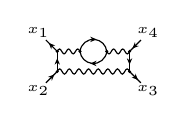
\begin{tikzpicture}[x=0.340cm, y=0.340cm, line width=0.420pt, baseline={([yshift=-0.6ex]0,0)}]
  \draw (-1.350,-0.500) -- (-1.350,0.250);
  \fill (-1.350,-0.006) -- (-1.452,-0.244) -- (-1.350,-0.167) -- (-1.248,-0.244) -- cycle;
  \draw (1.350,0.250) -- (1.350,-0.500);
  \fill (1.350,-0.244) -- (1.452,-0.006) -- (1.350,-0.083) -- (1.248,-0.006) -- cycle;
  \draw (0.500,0.250) arc[start angle=353.974, end angle=186.026, radius=0.503];
  \fill (-0.119,-0.200) -- (0.119,-0.302) -- (0.042,-0.200) -- (0.119,-0.098) -- cycle;
  \draw (-0.500,0.250) arc[start angle=173.974, end angle=6.026, radius=0.503];
  \fill (0.119,0.700) -- (-0.119,0.802) -- (-0.042,0.700) -- (-0.119,0.598) -- cycle;
  \draw plot[smooth, tension=0.7] coordinates {(-1.350,0.250) (-1.308,0.315) (-1.265,0.342) (-1.223,0.315) (-1.180,0.250) (-1.138,0.185) (-1.095,0.158) (-1.052,0.185) (-1.010,0.250) (-0.968,0.315) (-0.925,0.342) (-0.883,0.315) (-0.840,0.250) (-0.798,0.185) (-0.755,0.158) (-0.713,0.185) (-0.670,0.250) (-0.628,0.315) (-0.585,0.342) (-0.543,0.315) (-0.500,0.250)};
  \draw plot[smooth, tension=0.7] coordinates {(-1.350,-0.500) (-1.305,-0.431) (-1.260,-0.403) (-1.215,-0.431) (-1.170,-0.500) (-1.125,-0.569) (-1.080,-0.597) (-1.035,-0.569) (-0.990,-0.500) (-0.945,-0.431) (-0.900,-0.403) (-0.855,-0.431) (-0.810,-0.500) (-0.765,-0.569) (-0.720,-0.597) (-0.675,-0.569) (-0.630,-0.500) (-0.585,-0.431) (-0.540,-0.403) (-0.495,-0.431) (-0.450,-0.500) (-0.405,-0.569) (-0.360,-0.597) (-0.315,-0.569) (-0.270,-0.500) (-0.225,-0.431) (-0.180,-0.403) (-0.135,-0.431) (-0.090,-0.500) (-0.045,-0.569) (0.000,-0.597) (0.045,-0.569) (0.090,-0.500) (0.135,-0.431) (0.180,-0.403) (0.225,-0.431) (0.270,-0.500) (0.315,-0.569) (0.360,-0.597) (0.405,-0.569) (0.450,-0.500) (0.495,-0.431) (0.540,-0.403) (0.585,-0.431) (0.630,-0.500) (0.675,-0.569) (0.720,-0.597) (0.765,-0.569) (0.810,-0.500) (0.855,-0.431) (0.900,-0.403) (0.945,-0.431) (0.990,-0.500) (1.035,-0.569) (1.080,-0.597) (1.125,-0.569) (1.170,-0.500) (1.215,-0.431) (1.260,-0.403) (1.305,-0.431) (1.350,-0.500)};
  \draw plot[smooth, tension=0.7] coordinates {(1.350,0.250) (1.308,0.185) (1.265,0.158) (1.223,0.185) (1.180,0.250) (1.138,0.315) (1.095,0.342) (1.052,0.315) (1.010,0.250) (0.968,0.185) (0.925,0.158) (0.883,0.185) (0.840,0.250) (0.798,0.315) (0.755,0.342) (0.712,0.315) (0.670,0.250) (0.628,0.185) (0.585,0.158) (0.542,0.185) (0.500,0.250)};
  \draw (-1.350,0.250) -- (-1.774,0.674);
  \fill (-1.668,0.568) -- (-1.571,0.327) -- (-1.554,0.454) -- (-1.427,0.471) -- cycle;
  \draw (-1.350,-0.500) -- (-1.774,-0.924);
  \fill (-1.456,-0.606) -- (-1.697,-0.703) -- (-1.570,-0.720) -- (-1.553,-0.847) -- cycle;
  \draw (1.350,-0.500) -- (1.774,-0.924);
  \fill (1.668,-0.818) -- (1.571,-0.577) -- (1.554,-0.704) -- (1.427,-0.721) -- cycle;
  \draw (1.350,0.250) -- (1.774,0.674);
  \fill (1.456,0.356) -- (1.697,0.453) -- (1.570,0.470) -- (1.553,0.597) -- cycle;
  \fill (-1.350,0.250) circle (0.064);
  \fill (-1.350,-0.500) circle (0.064);
  \fill (1.350,-0.500) circle (0.064);
  \fill (1.350,0.250) circle (0.064);
  \fill (-0.500,0.250) circle (0.064);
  \fill (0.500,0.250) circle (0.064);
  \node[font=\tiny, inner sep=0pt, anchor=315] at (-1.838,0.738) {$x_{1}$};
  \node[font=\tiny, inner sep=0pt, anchor=45] at (-1.838,-0.988) {$x_{2}$};
  \node[font=\tiny, inner sep=0pt, anchor=135] at (1.838,-0.988) {$x_{3}$};
  \node[font=\tiny, inner sep=0pt, anchor=225] at (1.838,0.738) {$x_{4}$};
\end{tikzpicture}}
\diagramgap
\mbox{$\displaystyle +\,$\,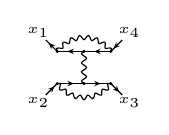
\begin{tikzpicture}[x=0.340cm, y=0.340cm, line width=0.420pt, baseline={([yshift=-0.6ex]0,0)}]
  \draw (0.000,0.600) -- (-1.000,0.600);
  \fill (-0.619,0.600) -- (-0.381,0.498) -- (-0.458,0.600) -- (-0.381,0.702) -- cycle;
  \draw (0.000,-0.600) -- (1.000,-0.600);
  \fill (0.619,-0.600) -- (0.381,-0.498) -- (0.458,-0.600) -- (0.381,-0.702) -- cycle;
  \draw (-1.000,-0.600) -- (0.000,-0.600);
  \fill (-0.381,-0.600) -- (-0.619,-0.498) -- (-0.542,-0.600) -- (-0.619,-0.702) -- cycle;
  \draw (1.000,0.600) -- (0.000,0.600);
  \fill (0.381,0.600) -- (0.619,0.498) -- (0.542,0.600) -- (0.619,0.702) -- cycle;
  \draw plot[smooth, tension=0.7] coordinates {(-1.000,0.600) (-1.023,0.666) (-1.017,0.713) (-0.972,0.730) (-0.902,0.722) (-0.834,0.710) (-0.792,0.719) (-0.781,0.762) (-0.790,0.830) (-0.796,0.900) (-0.777,0.944) (-0.730,0.949) (-0.665,0.923) (-0.602,0.895) (-0.558,0.893) (-0.537,0.931) (-0.529,1.000) (-0.516,1.069) (-0.488,1.107) (-0.441,1.099) (-0.384,1.058) (-0.330,1.015) (-0.288,1.002) (-0.258,1.034) (-0.233,1.098) (-0.204,1.161) (-0.166,1.191) (-0.122,1.172) (-0.078,1.118) (-0.037,1.062) (0.000,1.039) (0.037,1.062) (0.078,1.118) (0.122,1.172) (0.166,1.191) (0.204,1.161) (0.233,1.098) (0.258,1.034) (0.288,1.002) (0.330,1.015) (0.384,1.058) (0.441,1.099) (0.488,1.107) (0.516,1.069) (0.529,1.000) (0.537,0.931) (0.558,0.893) (0.602,0.895) (0.665,0.923) (0.730,0.949) (0.777,0.944) (0.796,0.900) (0.790,0.830) (0.781,0.762) (0.792,0.719) (0.834,0.710) (0.902,0.722) (0.972,0.730) (1.017,0.713) (1.023,0.666) (1.000,0.600)};
  \draw plot[smooth, tension=0.7] coordinates {(-1.000,-0.600) (-0.931,-0.597) (-0.890,-0.612) (-0.885,-0.655) (-0.902,-0.722) (-0.917,-0.790) (-0.904,-0.836) (-0.858,-0.847) (-0.790,-0.830) (-0.724,-0.810) (-0.680,-0.814) (-0.664,-0.854) (-0.665,-0.923) (-0.661,-0.993) (-0.638,-1.034) (-0.590,-1.033) (-0.529,-1.000) (-0.470,-0.963) (-0.427,-0.956) (-0.401,-0.991) (-0.384,-1.058) (-0.363,-1.125) (-0.330,-1.159) (-0.284,-1.146) (-0.233,-1.098) (-0.185,-1.048) (-0.145,-1.029) (-0.111,-1.057) (-0.078,-1.118) (-0.041,-1.177) (0.000,-1.201) (0.041,-1.177) (0.078,-1.118) (0.111,-1.057) (0.145,-1.029) (0.185,-1.048) (0.233,-1.098) (0.284,-1.146) (0.330,-1.159) (0.363,-1.125) (0.384,-1.058) (0.401,-0.991) (0.427,-0.956) (0.470,-0.963) (0.529,-1.000) (0.590,-1.033) (0.638,-1.034) (0.661,-0.993) (0.665,-0.923) (0.664,-0.854) (0.680,-0.814) (0.724,-0.810) (0.790,-0.830) (0.858,-0.847) (0.904,-0.836) (0.917,-0.790) (0.902,-0.722) (0.885,-0.655) (0.890,-0.612) (0.931,-0.597) (1.000,-0.600)};
  \draw plot[smooth, tension=0.7] coordinates {(0.000,-0.600) (-0.065,-0.557) (-0.093,-0.514) (-0.065,-0.471) (0.000,-0.429) (0.065,-0.386) (0.093,-0.343) (0.065,-0.300) (0.000,-0.257) (-0.065,-0.214) (-0.093,-0.171) (-0.065,-0.129) (0.000,-0.086) (0.065,-0.043) (0.093,0.000) (0.065,0.043) (0.000,0.086) (-0.065,0.129) (-0.093,0.171) (-0.065,0.214) (0.000,0.257) (0.065,0.300) (0.093,0.343) (0.065,0.386) (0.000,0.429) (-0.065,0.471) (-0.093,0.514) (-0.065,0.557) (0.000,0.600)};
  \draw (-1.000,0.600) -- (-1.424,1.024);
  \fill (-1.318,0.918) -- (-1.221,0.677) -- (-1.204,0.804) -- (-1.077,0.821) -- cycle;
  \draw (-1.000,-0.600) -- (-1.424,-1.024);
  \fill (-1.106,-0.706) -- (-1.347,-0.803) -- (-1.220,-0.820) -- (-1.203,-0.947) -- cycle;
  \draw (1.000,-0.600) -- (1.424,-1.024);
  \fill (1.318,-0.918) -- (1.221,-0.677) -- (1.204,-0.804) -- (1.077,-0.821) -- cycle;
  \draw (1.000,0.600) -- (1.424,1.024);
  \fill (1.106,0.706) -- (1.347,0.803) -- (1.220,0.820) -- (1.203,0.947) -- cycle;
  \fill (-1.000,0.600) circle (0.064);
  \fill (-1.000,-0.600) circle (0.064);
  \fill (1.000,-0.600) circle (0.064);
  \fill (1.000,0.600) circle (0.064);
  \fill (0.000,-0.600) circle (0.064);
  \fill (0.000,0.600) circle (0.064);
  \node[font=\tiny, inner sep=0pt, anchor=315] at (-1.488,1.088) {$x_{1}$};
  \node[font=\tiny, inner sep=0pt, anchor=45] at (-1.488,-1.088) {$x_{2}$};
  \node[font=\tiny, inner sep=0pt, anchor=135] at (1.488,-1.088) {$x_{3}$};
  \node[font=\tiny, inner sep=0pt, anchor=225] at (1.488,1.088) {$x_{4}$};
\end{tikzpicture}}
\diagramgap
\mbox{$\displaystyle -\,$\,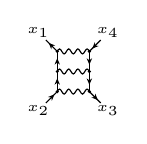
\begin{tikzpicture}[x=0.340cm, y=0.340cm, line width=0.420pt, baseline={([yshift=-0.6ex]0,0)}]
  \draw (-0.600,0.000) -- (-0.600,0.750);
  \fill (-0.600,0.494) -- (-0.702,0.256) -- (-0.600,0.333) -- (-0.498,0.256) -- cycle;
  \draw (0.600,0.000) -- (0.600,-0.750);
  \fill (0.600,-0.494) -- (0.702,-0.256) -- (0.600,-0.333) -- (0.498,-0.256) -- cycle;
  \draw (-0.600,-0.750) -- (-0.600,0.000);
  \fill (-0.600,-0.256) -- (-0.702,-0.494) -- (-0.600,-0.417) -- (-0.498,-0.494) -- cycle;
  \draw (0.600,0.750) -- (0.600,0.000);
  \fill (0.600,0.256) -- (0.702,0.494) -- (0.600,0.417) -- (0.498,0.494) -- cycle;
  \draw plot[smooth, tension=0.7] coordinates {(-0.600,0.750) (-0.557,0.815) (-0.514,0.843) (-0.471,0.815) (-0.429,0.750) (-0.386,0.685) (-0.343,0.657) (-0.300,0.685) (-0.257,0.750) (-0.214,0.815) (-0.171,0.843) (-0.129,0.815) (-0.086,0.750) (-0.043,0.685) (0.000,0.657) (0.043,0.685) (0.086,0.750) (0.129,0.815) (0.171,0.843) (0.214,0.815) (0.257,0.750) (0.300,0.685) (0.343,0.657) (0.386,0.685) (0.429,0.750) (0.471,0.815) (0.514,0.843) (0.557,0.815) (0.600,0.750)};
  \draw plot[smooth, tension=0.7] coordinates {(-0.600,-0.750) (-0.557,-0.685) (-0.514,-0.657) (-0.471,-0.685) (-0.429,-0.750) (-0.386,-0.815) (-0.343,-0.843) (-0.300,-0.815) (-0.257,-0.750) (-0.214,-0.685) (-0.171,-0.657) (-0.129,-0.685) (-0.086,-0.750) (-0.043,-0.815) (0.000,-0.843) (0.043,-0.815) (0.086,-0.750) (0.129,-0.685) (0.171,-0.657) (0.214,-0.685) (0.257,-0.750) (0.300,-0.815) (0.343,-0.843) (0.386,-0.815) (0.429,-0.750) (0.471,-0.685) (0.514,-0.657) (0.557,-0.685) (0.600,-0.750)};
  \draw plot[smooth, tension=0.7] coordinates {(-0.600,0.000) (-0.557,0.065) (-0.514,0.093) (-0.471,0.065) (-0.429,0.000) (-0.386,-0.065) (-0.343,-0.093) (-0.300,-0.065) (-0.257,0.000) (-0.214,0.065) (-0.171,0.093) (-0.129,0.065) (-0.086,0.000) (-0.043,-0.065) (0.000,-0.093) (0.043,-0.065) (0.086,0.000) (0.129,0.065) (0.171,0.093) (0.214,0.065) (0.257,0.000) (0.300,-0.065) (0.343,-0.093) (0.386,-0.065) (0.429,0.000) (0.471,0.065) (0.514,0.093) (0.557,0.065) (0.600,0.000)};
  \draw (-0.600,0.750) -- (-1.024,1.174);
  \fill (-0.918,1.068) -- (-0.821,0.827) -- (-0.804,0.954) -- (-0.677,0.971) -- cycle;
  \draw (-0.600,-0.750) -- (-1.024,-1.174);
  \fill (-0.706,-0.856) -- (-0.947,-0.953) -- (-0.820,-0.970) -- (-0.803,-1.097) -- cycle;
  \draw (0.600,-0.750) -- (1.024,-1.174);
  \fill (0.918,-1.068) -- (0.821,-0.827) -- (0.804,-0.954) -- (0.677,-0.971) -- cycle;
  \draw (0.600,0.750) -- (1.024,1.174);
  \fill (0.706,0.856) -- (0.947,0.953) -- (0.820,0.970) -- (0.803,1.097) -- cycle;
  \fill (-0.600,0.750) circle (0.064);
  \fill (-0.600,-0.750) circle (0.064);
  \fill (0.600,-0.750) circle (0.064);
  \fill (0.600,0.750) circle (0.064);
  \fill (-0.600,0.000) circle (0.064);
  \fill (0.600,0.000) circle (0.064);
  \node[font=\tiny, inner sep=0pt, anchor=315] at (-1.088,1.238) {$x_{1}$};
  \node[font=\tiny, inner sep=0pt, anchor=45] at (-1.088,-1.238) {$x_{2}$};
  \node[font=\tiny, inner sep=0pt, anchor=135] at (1.088,-1.238) {$x_{3}$};
  \node[font=\tiny, inner sep=0pt, anchor=225] at (1.088,1.238) {$x_{4}$};
\end{tikzpicture}}
\diagramgap
\mbox{$\displaystyle -\,$\,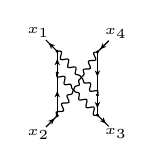
\begin{tikzpicture}[x=0.340cm, y=0.340cm, line width=0.420pt, baseline={([yshift=-0.6ex]0,0)}]
  \draw (-0.750,0.404) -- (-0.750,1.204);
  \fill (-0.750,0.924) -- (-0.852,0.685) -- (-0.750,0.762) -- (-0.648,0.685) -- cycle;
  \draw (0.750,-0.421) -- (0.750,-1.171);
  \fill (0.750,-0.915) -- (0.852,-0.676) -- (0.750,-0.754) -- (0.648,-0.676) -- cycle;
  \draw (-0.750,-1.196) -- (-0.750,0.404);
  \fill (-0.750,-0.276) -- (-0.852,-0.515) -- (-0.750,-0.438) -- (-0.648,-0.515) -- cycle;
  \draw (0.750,1.179) -- (0.750,-0.421);
  \fill (0.750,0.260) -- (0.852,0.499) -- (0.750,0.421) -- (0.648,0.499) -- cycle;
  \draw plot[smooth, tension=0.7] coordinates {(-0.750,1.204) (-0.660,1.219) (-0.602,1.204) (-0.591,1.145) (-0.614,1.056) (-0.636,0.967) (-0.625,0.909) (-0.568,0.894) (-0.477,0.909) (-0.387,0.924) (-0.329,0.908) (-0.319,0.850) (-0.341,0.761) (-0.363,0.672) (-0.353,0.613) (-0.295,0.598) (-0.205,0.613) (-0.114,0.628) (-0.057,0.613) (-0.046,0.555) (-0.068,0.466) (-0.082,0.385) (-0.053,0.343) (0.008,0.331) (0.068,0.318) (0.108,0.286) (0.137,0.245) (0.172,0.208) (0.205,0.170) (0.222,0.118) (0.233,0.059) (0.267,0.023) (0.341,0.022) (0.430,0.036) (0.489,0.022) (0.500,-0.036) (0.477,-0.125) (0.455,-0.214) (0.466,-0.273) (0.523,-0.288) (0.614,-0.273) (0.704,-0.258) (0.762,-0.273) (0.772,-0.332) (0.750,-0.421)};
  \draw plot[smooth, tension=0.7] coordinates {(-0.750,-1.196) (-0.785,-1.118) (-0.786,-1.063) (-0.735,-1.039) (-0.650,-1.038) (-0.565,-1.036) (-0.514,-1.012) (-0.515,-0.957) (-0.550,-0.879) (-0.585,-0.801) (-0.586,-0.746) (-0.535,-0.722) (-0.450,-0.721) (-0.365,-0.719) (-0.314,-0.696) (-0.315,-0.640) (-0.350,-0.563) (-0.385,-0.485) (-0.382,-0.432) (-0.325,-0.412) (-0.250,-0.404) (-0.198,-0.381) (-0.179,-0.338) (-0.170,-0.289) (-0.150,-0.246) (-0.127,-0.205) (-0.112,-0.159) (-0.094,-0.115) (-0.050,-0.088) (0.019,-0.075) (0.070,-0.053) (0.071,0.002) (0.050,0.071) (0.052,0.125) (0.084,0.160) (0.122,0.192) (0.150,0.229) (0.178,0.267) (0.216,0.298) (0.248,0.334) (0.250,0.387) (0.228,0.457) (0.221,0.517) (0.265,0.544) (0.350,0.546) (0.435,0.547) (0.485,0.571) (0.485,0.626) (0.450,0.704) (0.415,0.782) (0.415,0.837) (0.465,0.861) (0.550,0.863) (0.635,0.864) (0.686,0.888) (0.685,0.943) (0.650,1.021) (0.615,1.099) (0.614,1.154) (0.665,1.178) (0.750,1.179)};
  \draw plot[smooth, tension=0.7] coordinates {(0.750,-1.171) (0.661,-1.187) (0.604,-1.173) (0.593,-1.116) (0.614,-1.028) (0.634,-0.940) (0.623,-0.882) (0.566,-0.868) (0.477,-0.884) (0.389,-0.901) (0.332,-0.887) (0.320,-0.829) (0.341,-0.741) (0.361,-0.653) (0.350,-0.596) (0.293,-0.582) (0.205,-0.598) (0.116,-0.614) (0.059,-0.600) (0.048,-0.543) (0.068,-0.455) (0.078,-0.377) (0.048,-0.338) (-0.012,-0.326) (-0.068,-0.312) (-0.106,-0.280) (-0.137,-0.240) (-0.172,-0.206) (-0.205,-0.169) (-0.220,-0.115) (-0.230,-0.057) (-0.266,-0.022) (-0.341,-0.025) (-0.429,-0.041) (-0.486,-0.027) (-0.498,0.030) (-0.477,0.118) (-0.457,0.206) (-0.468,0.263) (-0.525,0.277) (-0.614,0.261) (-0.702,0.245) (-0.759,0.259) (-0.771,0.316) (-0.750,0.404)};
  \draw (-0.750,1.204) -- (-1.174,1.628);
  \fill (-1.068,1.522) -- (-0.971,1.281) -- (-0.954,1.408) -- (-0.827,1.425) -- cycle;
  \draw (-0.750,-1.196) -- (-1.174,-1.620);
  \fill (-0.856,-1.302) -- (-1.097,-1.399) -- (-0.970,-1.416) -- (-0.953,-1.543) -- cycle;
  \draw (0.750,-1.171) -- (1.174,-1.595);
  \fill (1.068,-1.489) -- (0.971,-1.248) -- (0.954,-1.375) -- (0.827,-1.392) -- cycle;
  \draw (0.750,1.179) -- (1.174,1.603);
  \fill (0.856,1.286) -- (1.097,1.382) -- (0.970,1.400) -- (0.953,1.527) -- cycle;
  \fill (-0.750,1.204) circle (0.064);
  \fill (-0.750,-1.196) circle (0.064);
  \fill (0.750,-1.171) circle (0.064);
  \fill (0.750,1.179) circle (0.064);
  \fill (-0.750,0.404) circle (0.064);
  \fill (0.750,-0.421) circle (0.064);
  \node[font=\tiny, inner sep=0pt, anchor=315] at (-1.238,1.692) {$x_{1}$};
  \node[font=\tiny, inner sep=0pt, anchor=45] at (-1.238,-1.684) {$x_{2}$};
  \node[font=\tiny, inner sep=0pt, anchor=135] at (1.238,-1.659) {$x_{3}$};
  \node[font=\tiny, inner sep=0pt, anchor=225] at (1.238,1.667) {$x_{4}$};
\end{tikzpicture}}
\diagramgap
\mbox{$\displaystyle +\,$\,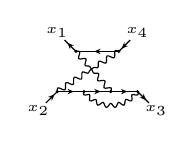
\begin{tikzpicture}[x=0.340cm, y=0.340cm, line width=0.420pt, baseline={([yshift=-0.6ex]0,0)}]
  \draw (0.800,1.000) -- (-0.800,1.000);
  \fill (-0.119,1.000) -- (0.119,0.898) -- (0.042,1.000) -- (0.119,1.102) -- cycle;
  \draw (0.500,-0.500) -- (1.500,-0.500);
  \fill (1.119,-0.500) -- (0.881,-0.398) -- (0.958,-0.500) -- (0.881,-0.602) -- cycle;
  \draw (-1.500,-0.500) -- (-0.500,-0.500);
  \fill (-0.881,-0.500) -- (-1.119,-0.398) -- (-1.042,-0.500) -- (-1.119,-0.602) -- cycle;
  \draw (-0.500,-0.500) -- (0.500,-0.500);
  \fill (0.119,-0.500) -- (-0.119,-0.398) -- (-0.042,-0.500) -- (-0.119,-0.602) -- cycle;
  \draw plot[smooth, tension=0.7] coordinates {(-0.800,1.000) (-0.718,1.011) (-0.667,0.996) (-0.659,0.943) (-0.682,0.864) (-0.704,0.784) (-0.696,0.732) (-0.645,0.716) (-0.564,0.727) (-0.482,0.738) (-0.431,0.723) (-0.423,0.670) (-0.445,0.591) (-0.467,0.513) (-0.450,0.467) (-0.393,0.457) (-0.327,0.455) (-0.283,0.433) (-0.259,0.394) (-0.238,0.353) (-0.209,0.318) (-0.185,0.279) (-0.170,0.233) (-0.145,0.195) (-0.091,0.182) (-0.017,0.186) (0.040,0.175) (0.050,0.125) (0.027,0.045) (0.005,-0.034) (0.013,-0.087) (0.064,-0.102) (0.145,-0.091) (0.227,-0.080) (0.278,-0.095) (0.286,-0.148) (0.264,-0.227) (0.241,-0.306) (0.249,-0.359) (0.300,-0.375) (0.382,-0.364) (0.463,-0.353) (0.515,-0.368) (0.523,-0.421) (0.500,-0.500)};
  \draw plot[smooth, tension=0.7] coordinates {(-1.500,-0.500) (-1.500,-0.416) (-1.477,-0.367) (-1.423,-0.366) (-1.347,-0.400) (-1.270,-0.434) (-1.216,-0.433) (-1.193,-0.384) (-1.193,-0.300) (-1.193,-0.216) (-1.171,-0.167) (-1.117,-0.166) (-1.040,-0.200) (-0.963,-0.234) (-0.909,-0.233) (-0.887,-0.184) (-0.887,-0.100) (-0.887,-0.016) (-0.864,0.033) (-0.810,0.034) (-0.733,0.000) (-0.657,-0.034) (-0.603,-0.033) (-0.580,0.016) (-0.580,0.100) (-0.580,0.184) (-0.557,0.233) (-0.502,0.231) (-0.427,0.200) (-0.363,0.187) (-0.326,0.213) (-0.302,0.261) (-0.273,0.300) (-0.235,0.325) (-0.198,0.352) (-0.164,0.383) (-0.120,0.400) (-0.062,0.395) (-0.005,0.391) (0.029,0.423) (0.033,0.500) (0.033,0.584) (0.056,0.633) (0.110,0.634) (0.187,0.600) (0.263,0.566) (0.317,0.567) (0.340,0.616) (0.340,0.700) (0.340,0.784) (0.363,0.833) (0.417,0.834) (0.493,0.800) (0.570,0.766) (0.624,0.767) (0.647,0.816) (0.647,0.900) (0.647,0.984) (0.669,1.033) (0.723,1.034) (0.800,1.000)};
  \draw plot[smooth, tension=0.7] coordinates {(1.500,-0.500) (1.523,-0.566) (1.517,-0.613) (1.472,-0.630) (1.402,-0.622) (1.334,-0.610) (1.292,-0.619) (1.281,-0.662) (1.290,-0.730) (1.296,-0.800) (1.277,-0.844) (1.230,-0.849) (1.165,-0.823) (1.102,-0.795) (1.058,-0.793) (1.037,-0.831) (1.029,-0.900) (1.016,-0.969) (0.988,-1.007) (0.941,-0.999) (0.884,-0.958) (0.830,-0.915) (0.788,-0.902) (0.758,-0.934) (0.733,-0.998) (0.704,-1.061) (0.666,-1.091) (0.622,-1.072) (0.578,-1.018) (0.537,-0.962) (0.500,-0.939) (0.463,-0.962) (0.422,-1.018) (0.378,-1.072) (0.334,-1.091) (0.296,-1.061) (0.267,-0.998) (0.242,-0.934) (0.212,-0.902) (0.170,-0.915) (0.116,-0.958) (0.059,-0.999) (0.012,-1.007) (-0.016,-0.969) (-0.029,-0.900) (-0.037,-0.831) (-0.058,-0.793) (-0.102,-0.795) (-0.165,-0.823) (-0.230,-0.849) (-0.277,-0.844) (-0.296,-0.800) (-0.290,-0.730) (-0.281,-0.662) (-0.292,-0.619) (-0.334,-0.610) (-0.402,-0.622) (-0.472,-0.630) (-0.517,-0.613) (-0.523,-0.566) (-0.500,-0.500)};
  \draw (-0.800,1.000) -- (-1.224,1.424);
  \fill (-1.118,1.318) -- (-1.021,1.077) -- (-1.004,1.204) -- (-0.877,1.221) -- cycle;
  \draw (-1.500,-0.500) -- (-1.924,-0.924);
  \fill (-1.606,-0.606) -- (-1.847,-0.703) -- (-1.720,-0.720) -- (-1.703,-0.847) -- cycle;
  \draw (1.500,-0.500) -- (1.924,-0.924);
  \fill (1.818,-0.818) -- (1.721,-0.577) -- (1.704,-0.704) -- (1.577,-0.721) -- cycle;
  \draw (0.800,1.000) -- (1.224,1.424);
  \fill (0.906,1.106) -- (1.147,1.203) -- (1.020,1.220) -- (1.003,1.347) -- cycle;
  \fill (-0.800,1.000) circle (0.064);
  \fill (-1.500,-0.500) circle (0.064);
  \fill (1.500,-0.500) circle (0.064);
  \fill (0.800,1.000) circle (0.064);
  \fill (-0.500,-0.500) circle (0.064);
  \fill (0.500,-0.500) circle (0.064);
  \node[font=\tiny, inner sep=0pt, anchor=315] at (-1.288,1.488) {$x_{1}$};
  \node[font=\tiny, inner sep=0pt, anchor=45] at (-1.988,-0.988) {$x_{2}$};
  \node[font=\tiny, inner sep=0pt, anchor=135] at (1.988,-0.988) {$x_{3}$};
  \node[font=\tiny, inner sep=0pt, anchor=225] at (1.288,1.488) {$x_{4}$};
\end{tikzpicture}}
\diagramgap
\mbox{$\displaystyle -\,$\,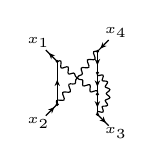
\begin{tikzpicture}[x=0.340cm, y=0.340cm, line width=0.420pt, baseline={([yshift=-0.6ex]0,0)}]
  \draw (-1.000,-0.792) -- (-1.000,0.808);
  \fill (-1.000,0.128) -- (-1.102,-0.111) -- (-1.000,-0.033) -- (-0.898,-0.111) -- cycle;
  \draw (0.500,-0.417) -- (0.500,-1.167);
  \fill (0.500,-0.911) -- (0.602,-0.672) -- (0.500,-0.750) -- (0.398,-0.672) -- cycle;
  \draw (0.500,1.183) -- (0.500,0.383);
  \fill (0.500,0.664) -- (0.602,0.903) -- (0.500,0.825) -- (0.398,0.903) -- cycle;
  \draw (0.500,0.383) -- (0.500,-0.417);
  \fill (0.500,-0.136) -- (0.602,0.103) -- (0.500,0.025) -- (0.398,0.103) -- cycle;
  \draw plot[smooth, tension=0.7] coordinates {(-1.000,0.808) (-0.923,0.833) (-0.872,0.826) (-0.855,0.777) (-0.864,0.697) (-0.872,0.617) (-0.856,0.568) (-0.804,0.561) (-0.727,0.586) (-0.651,0.610) (-0.599,0.604) (-0.582,0.554) (-0.591,0.474) (-0.599,0.394) (-0.583,0.345) (-0.531,0.339) (-0.455,0.363) (-0.387,0.375) (-0.351,0.350) (-0.336,0.299) (-0.318,0.252) (-0.286,0.221) (-0.250,0.196) (-0.218,0.165) (-0.182,0.140) (-0.132,0.132) (-0.079,0.127) (-0.047,0.097) (-0.045,0.029) (-0.054,-0.051) (-0.037,-0.101) (0.014,-0.107) (0.091,-0.083) (0.168,-0.058) (0.219,-0.065) (0.236,-0.114) (0.227,-0.194) (0.219,-0.274) (0.235,-0.323) (0.287,-0.330) (0.364,-0.305) (0.440,-0.281) (0.492,-0.287) (0.508,-0.337) (0.500,-0.417)};
  \draw plot[smooth, tension=0.7] coordinates {(-1.000,-0.792) (-1.029,-0.710) (-1.024,-0.653) (-0.971,-0.634) (-0.885,-0.640) (-0.798,-0.646) (-0.745,-0.626) (-0.740,-0.570) (-0.769,-0.488) (-0.798,-0.406) (-0.794,-0.350) (-0.741,-0.330) (-0.654,-0.336) (-0.567,-0.342) (-0.514,-0.322) (-0.509,-0.266) (-0.538,-0.184) (-0.568,-0.102) (-0.563,-0.046) (-0.510,-0.026) (-0.423,-0.032) (-0.349,-0.028) (-0.318,0.008) (-0.315,0.065) (-0.308,0.120) (-0.282,0.160) (-0.250,0.196) (-0.224,0.236) (-0.192,0.272) (-0.142,0.293) (-0.087,0.311) (-0.061,0.352) (-0.077,0.424) (-0.106,0.506) (-0.101,0.562) (-0.048,0.582) (0.038,0.576) (0.125,0.570) (0.178,0.589) (0.183,0.646) (0.154,0.728) (0.125,0.810) (0.130,0.866) (0.182,0.886) (0.269,0.879) (0.356,0.873) (0.409,0.893) (0.414,0.949) (0.385,1.031) (0.355,1.113) (0.360,1.170) (0.413,1.189) (0.500,1.183)};
  \draw plot[smooth, tension=0.7] coordinates {(0.500,-1.167) (0.497,-1.105) (0.510,-1.068) (0.548,-1.063) (0.608,-1.078) (0.670,-1.090) (0.711,-1.077) (0.719,-1.035) (0.702,-0.975) (0.681,-0.917) (0.683,-0.878) (0.718,-0.862) (0.780,-0.859) (0.842,-0.852) (0.877,-0.828) (0.873,-0.786) (0.839,-0.733) (0.803,-0.683) (0.793,-0.646) (0.822,-0.620) (0.880,-0.599) (0.937,-0.575) (0.965,-0.542) (0.948,-0.502) (0.900,-0.461) (0.851,-0.425) (0.830,-0.392) (0.851,-0.359) (0.900,-0.322) (0.948,-0.281) (0.965,-0.242) (0.937,-0.209) (0.880,-0.184) (0.822,-0.163) (0.793,-0.137) (0.803,-0.100) (0.839,-0.050) (0.873,0.002) (0.877,0.045) (0.842,0.069) (0.780,0.076) (0.718,0.079) (0.683,0.095) (0.681,0.134) (0.702,0.192) (0.719,0.252) (0.711,0.294) (0.670,0.306) (0.608,0.295) (0.548,0.280) (0.510,0.285) (0.497,0.322) (0.500,0.383)};
  \draw (-1.000,0.808) -- (-1.424,1.233);
  \fill (-1.318,1.126) -- (-1.221,0.885) -- (-1.204,1.012) -- (-1.077,1.029) -- cycle;
  \draw (-1.000,-0.792) -- (-1.424,-1.216);
  \fill (-1.106,-0.898) -- (-1.347,-0.995) -- (-1.220,-1.012) -- (-1.203,-1.139) -- cycle;
  \draw (0.500,-1.167) -- (0.924,-1.591);
  \fill (0.818,-1.484) -- (0.721,-1.243) -- (0.704,-1.370) -- (0.577,-1.388) -- cycle;
  \draw (0.500,1.183) -- (0.924,1.608);
  \fill (0.606,1.290) -- (0.847,1.387) -- (0.720,1.404) -- (0.703,1.531) -- cycle;
  \fill (-1.000,0.808) circle (0.064);
  \fill (-1.000,-0.792) circle (0.064);
  \fill (0.500,-1.167) circle (0.064);
  \fill (0.500,1.183) circle (0.064);
  \fill (0.500,0.383) circle (0.064);
  \fill (0.500,-0.417) circle (0.064);
  \node[font=\tiny, inner sep=0pt, anchor=315] at (-1.488,1.296) {$x_{1}$};
  \node[font=\tiny, inner sep=0pt, anchor=45] at (-1.488,-1.280) {$x_{2}$};
  \node[font=\tiny, inner sep=0pt, anchor=135] at (0.988,-1.655) {$x_{3}$};
  \node[font=\tiny, inner sep=0pt, anchor=225] at (0.988,1.671) {$x_{4}$};
\end{tikzpicture}}
\diagramgap
\mbox{$\displaystyle +\,$\,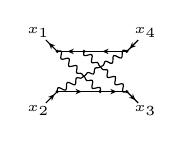
\begin{tikzpicture}[x=0.340cm, y=0.340cm, line width=0.420pt, baseline={([yshift=-0.6ex]0,0)}]
  \draw (-0.300,0.750) -- (-1.300,0.750);
  \fill (-0.919,0.750) -- (-0.681,0.648) -- (-0.758,0.750) -- (-0.681,0.852) -- cycle;
  \draw (0.300,-0.750) -- (1.300,-0.750);
  \fill (0.919,-0.750) -- (0.681,-0.648) -- (0.758,-0.750) -- (0.681,-0.852) -- cycle;
  \draw (-1.300,-0.750) -- (0.300,-0.750);
  \fill (-0.381,-0.750) -- (-0.619,-0.648) -- (-0.542,-0.750) -- (-0.619,-0.852) -- cycle;
  \draw (1.300,0.750) -- (-0.300,0.750);
  \fill (0.381,0.750) -- (0.619,0.648) -- (0.542,0.750) -- (0.619,0.852) -- cycle;
  \draw plot[smooth, tension=0.7] coordinates {(-1.300,0.750) (-1.212,0.771) (-1.154,0.760) (-1.139,0.703) (-1.155,0.614) (-1.170,0.524) (-1.155,0.467) (-1.098,0.456) (-1.009,0.477) (-0.921,0.499) (-0.863,0.488) (-0.848,0.431) (-0.864,0.341) (-0.879,0.251) (-0.865,0.194) (-0.807,0.183) (-0.718,0.205) (-0.630,0.226) (-0.572,0.215) (-0.557,0.158) (-0.573,0.068) (-0.586,-0.019) (-0.560,-0.064) (-0.497,-0.069) (-0.427,-0.068) (-0.379,-0.090) (-0.349,-0.130) (-0.318,-0.170) (-0.282,-0.205) (-0.253,-0.247) (-0.233,-0.299) (-0.201,-0.336) (-0.136,-0.341) (-0.053,-0.325) (0.009,-0.331) (0.025,-0.388) (0.009,-0.477) (-0.007,-0.567) (0.008,-0.624) (0.066,-0.635) (0.155,-0.614) (0.243,-0.592) (0.301,-0.603) (0.316,-0.660) (0.300,-0.750)};
  \draw plot[smooth, tension=0.7] coordinates {(-1.300,-0.750) (-1.295,-0.659) (-1.267,-0.606) (-1.208,-0.609) (-1.127,-0.650) (-1.045,-0.691) (-0.986,-0.694) (-0.958,-0.641) (-0.953,-0.550) (-0.948,-0.459) (-0.921,-0.406) (-0.862,-0.409) (-0.780,-0.450) (-0.698,-0.491) (-0.639,-0.494) (-0.612,-0.441) (-0.607,-0.350) (-0.598,-0.265) (-0.561,-0.230) (-0.498,-0.238) (-0.433,-0.250) (-0.384,-0.236) (-0.345,-0.204) (-0.303,-0.175) (-0.260,-0.150) (-0.225,-0.111) (-0.195,-0.062) (-0.153,-0.034) (-0.087,-0.050) (-0.007,-0.087) (0.054,-0.094) (0.079,-0.037) (0.087,0.050) (0.107,0.116) (0.151,0.138) (0.209,0.139) (0.260,0.150) (0.303,0.175) (0.349,0.196) (0.396,0.214) (0.433,0.250) (0.456,0.312) (0.479,0.370) (0.529,0.385) (0.607,0.350) (0.688,0.309) (0.747,0.306) (0.775,0.359) (0.780,0.450) (0.785,0.541) (0.813,0.594) (0.872,0.591) (0.953,0.550) (1.035,0.509) (1.094,0.506) (1.122,0.559) (1.127,0.650) (1.132,0.741) (1.159,0.794) (1.218,0.791) (1.300,0.750)};
  \draw plot[smooth, tension=0.7] coordinates {(1.300,-0.750) (1.212,-0.771) (1.154,-0.760) (1.139,-0.703) (1.155,-0.614) (1.170,-0.524) (1.155,-0.467) (1.098,-0.456) (1.009,-0.477) (0.921,-0.499) (0.863,-0.488) (0.848,-0.431) (0.864,-0.341) (0.879,-0.251) (0.865,-0.194) (0.807,-0.183) (0.718,-0.205) (0.630,-0.226) (0.572,-0.215) (0.557,-0.158) (0.573,-0.068) (0.586,0.019) (0.560,0.064) (0.497,0.069) (0.427,0.068) (0.379,0.090) (0.349,0.130) (0.318,0.170) (0.282,0.205) (0.253,0.247) (0.233,0.299) (0.201,0.336) (0.136,0.341) (0.053,0.325) (-0.009,0.331) (-0.025,0.388) (-0.009,0.477) (0.007,0.567) (-0.008,0.624) (-0.066,0.635) (-0.155,0.614) (-0.243,0.592) (-0.301,0.603) (-0.316,0.660) (-0.300,0.750)};
  \draw (-1.300,0.750) -- (-1.724,1.174);
  \fill (-1.618,1.068) -- (-1.521,0.827) -- (-1.504,0.954) -- (-1.377,0.971) -- cycle;
  \draw (-1.300,-0.750) -- (-1.724,-1.174);
  \fill (-1.406,-0.856) -- (-1.647,-0.953) -- (-1.520,-0.970) -- (-1.503,-1.097) -- cycle;
  \draw (1.300,-0.750) -- (1.724,-1.174);
  \fill (1.618,-1.068) -- (1.521,-0.827) -- (1.504,-0.954) -- (1.377,-0.971) -- cycle;
  \draw (1.300,0.750) -- (1.724,1.174);
  \fill (1.406,0.856) -- (1.647,0.953) -- (1.520,0.970) -- (1.503,1.097) -- cycle;
  \fill (-1.300,0.750) circle (0.064);
  \fill (-1.300,-0.750) circle (0.064);
  \fill (1.300,-0.750) circle (0.064);
  \fill (1.300,0.750) circle (0.064);
  \fill (0.300,-0.750) circle (0.064);
  \fill (-0.300,0.750) circle (0.064);
  \node[font=\tiny, inner sep=0pt, anchor=315] at (-1.788,1.238) {$x_{1}$};
  \node[font=\tiny, inner sep=0pt, anchor=45] at (-1.788,-1.238) {$x_{2}$};
  \node[font=\tiny, inner sep=0pt, anchor=135] at (1.788,-1.238) {$x_{3}$};
  \node[font=\tiny, inner sep=0pt, anchor=225] at (1.788,1.238) {$x_{4}$};
\end{tikzpicture}}
\diagramgap
\mbox{$\displaystyle -\,$\,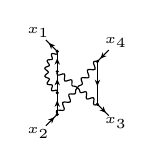
\begin{tikzpicture}[x=0.340cm, y=0.340cm, line width=0.420pt, baseline={([yshift=-0.6ex]0,0)}]
  \draw (-0.500,0.417) -- (-0.500,1.167);
  \fill (-0.500,0.911) -- (-0.602,0.672) -- (-0.500,0.750) -- (-0.398,0.672) -- cycle;
  \draw (1.000,0.792) -- (1.000,-0.808);
  \fill (1.000,-0.128) -- (1.102,0.111) -- (1.000,0.033) -- (0.898,0.111) -- cycle;
  \draw (-0.500,-1.183) -- (-0.500,-0.383);
  \fill (-0.500,-0.664) -- (-0.602,-0.903) -- (-0.500,-0.825) -- (-0.398,-0.903) -- cycle;
  \draw (-0.500,-0.383) -- (-0.500,0.417);
  \fill (-0.500,0.136) -- (-0.602,-0.103) -- (-0.500,-0.025) -- (-0.398,-0.103) -- cycle;
  \draw plot[smooth, tension=0.7] coordinates {(-0.500,1.167) (-0.497,1.105) (-0.510,1.068) (-0.548,1.063) (-0.608,1.078) (-0.670,1.090) (-0.711,1.077) (-0.719,1.035) (-0.702,0.975) (-0.681,0.917) (-0.683,0.878) (-0.718,0.862) (-0.780,0.859) (-0.842,0.852) (-0.877,0.828) (-0.873,0.786) (-0.839,0.733) (-0.803,0.683) (-0.793,0.646) (-0.822,0.620) (-0.880,0.599) (-0.937,0.575) (-0.965,0.542) (-0.948,0.502) (-0.900,0.461) (-0.851,0.425) (-0.830,0.392) (-0.851,0.359) (-0.900,0.322) (-0.948,0.281) (-0.965,0.242) (-0.937,0.209) (-0.880,0.184) (-0.822,0.163) (-0.793,0.137) (-0.803,0.100) (-0.839,0.050) (-0.873,-0.002) (-0.877,-0.045) (-0.842,-0.069) (-0.780,-0.076) (-0.718,-0.079) (-0.683,-0.095) (-0.681,-0.134) (-0.702,-0.192) (-0.719,-0.252) (-0.711,-0.294) (-0.670,-0.306) (-0.608,-0.295) (-0.548,-0.280) (-0.510,-0.285) (-0.497,-0.322) (-0.500,-0.383)};
  \draw plot[smooth, tension=0.7] coordinates {(-0.500,-1.183) (-0.529,-1.101) (-0.524,-1.045) (-0.471,-1.025) (-0.385,-1.031) (-0.298,-1.037) (-0.245,-1.018) (-0.240,-0.962) (-0.269,-0.879) (-0.298,-0.797) (-0.294,-0.741) (-0.241,-0.721) (-0.154,-0.728) (-0.067,-0.734) (-0.014,-0.714) (-0.009,-0.658) (-0.038,-0.576) (-0.068,-0.494) (-0.063,-0.437) (-0.010,-0.418) (0.077,-0.424) (0.151,-0.420) (0.182,-0.384) (0.185,-0.326) (0.192,-0.272) (0.218,-0.232) (0.250,-0.196) (0.276,-0.156) (0.308,-0.120) (0.358,-0.098) (0.413,-0.080) (0.439,-0.040) (0.423,0.032) (0.394,0.114) (0.399,0.170) (0.452,0.190) (0.538,0.184) (0.625,0.178) (0.678,0.198) (0.683,0.254) (0.654,0.336) (0.625,0.418) (0.630,0.474) (0.682,0.494) (0.769,0.488) (0.856,0.482) (0.909,0.501) (0.914,0.558) (0.885,0.640) (0.855,0.722) (0.860,0.778) (0.913,0.798) (1.000,0.792)};
  \draw plot[smooth, tension=0.7] coordinates {(1.000,-0.808) (0.923,-0.833) (0.872,-0.826) (0.855,-0.777) (0.864,-0.697) (0.872,-0.617) (0.856,-0.568) (0.804,-0.561) (0.727,-0.586) (0.651,-0.610) (0.599,-0.604) (0.582,-0.554) (0.591,-0.474) (0.599,-0.394) (0.583,-0.345) (0.531,-0.339) (0.455,-0.363) (0.387,-0.375) (0.351,-0.350) (0.336,-0.299) (0.318,-0.252) (0.286,-0.221) (0.250,-0.196) (0.218,-0.165) (0.182,-0.140) (0.132,-0.132) (0.079,-0.127) (0.047,-0.097) (0.045,-0.029) (0.054,0.051) (0.037,0.101) (-0.014,0.107) (-0.091,0.083) (-0.168,0.058) (-0.219,0.065) (-0.236,0.114) (-0.227,0.194) (-0.219,0.274) (-0.235,0.323) (-0.287,0.330) (-0.364,0.305) (-0.440,0.281) (-0.492,0.287) (-0.508,0.337) (-0.500,0.417)};
  \draw (-0.500,1.167) -- (-0.924,1.591);
  \fill (-0.818,1.484) -- (-0.721,1.243) -- (-0.704,1.370) -- (-0.577,1.388) -- cycle;
  \draw (-0.500,-1.183) -- (-0.924,-1.608);
  \fill (-0.606,-1.290) -- (-0.847,-1.387) -- (-0.720,-1.404) -- (-0.703,-1.531) -- cycle;
  \draw (1.000,-0.808) -- (1.424,-1.233);
  \fill (1.318,-1.126) -- (1.221,-0.885) -- (1.204,-1.012) -- (1.077,-1.029) -- cycle;
  \draw (1.000,0.792) -- (1.424,1.216);
  \fill (1.106,0.898) -- (1.347,0.995) -- (1.220,1.012) -- (1.203,1.139) -- cycle;
  \fill (-0.500,1.167) circle (0.064);
  \fill (-0.500,-1.183) circle (0.064);
  \fill (1.000,-0.808) circle (0.064);
  \fill (1.000,0.792) circle (0.064);
  \fill (-0.500,-0.383) circle (0.064);
  \fill (-0.500,0.417) circle (0.064);
  \node[font=\tiny, inner sep=0pt, anchor=315] at (-0.988,1.655) {$x_{1}$};
  \node[font=\tiny, inner sep=0pt, anchor=45] at (-0.988,-1.671) {$x_{2}$};
  \node[font=\tiny, inner sep=0pt, anchor=135] at (1.488,-1.296) {$x_{3}$};
  \node[font=\tiny, inner sep=0pt, anchor=225] at (1.488,1.280) {$x_{4}$};
\end{tikzpicture}}
\diagramgap
\mbox{$\displaystyle +\,$\,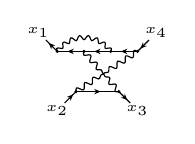
\begin{tikzpicture}[x=0.340cm, y=0.340cm, line width=0.420pt, baseline={([yshift=-0.6ex]0,0)}]
  \draw (-0.500,0.500) -- (-1.500,0.500);
  \fill (-1.119,0.500) -- (-0.881,0.398) -- (-0.958,0.500) -- (-0.881,0.602) -- cycle;
  \draw (-0.800,-1.000) -- (0.800,-1.000);
  \fill (0.119,-1.000) -- (-0.119,-0.898) -- (-0.042,-1.000) -- (-0.119,-1.102) -- cycle;
  \draw (1.500,0.500) -- (0.500,0.500);
  \fill (0.881,0.500) -- (1.119,0.398) -- (1.042,0.500) -- (1.119,0.602) -- cycle;
  \draw (0.500,0.500) -- (-0.500,0.500);
  \fill (-0.119,0.500) -- (0.119,0.398) -- (0.042,0.500) -- (0.119,0.602) -- cycle;
  \draw plot[smooth, tension=0.7] coordinates {(-1.500,0.500) (-1.523,0.566) (-1.517,0.613) (-1.472,0.630) (-1.402,0.622) (-1.334,0.610) (-1.292,0.619) (-1.281,0.662) (-1.290,0.730) (-1.296,0.800) (-1.277,0.844) (-1.230,0.849) (-1.165,0.823) (-1.102,0.795) (-1.058,0.793) (-1.037,0.831) (-1.029,0.900) (-1.016,0.969) (-0.988,1.007) (-0.941,0.999) (-0.884,0.958) (-0.830,0.915) (-0.788,0.902) (-0.758,0.934) (-0.733,0.998) (-0.704,1.061) (-0.666,1.091) (-0.622,1.072) (-0.578,1.018) (-0.537,0.962) (-0.500,0.939) (-0.463,0.962) (-0.422,1.018) (-0.378,1.072) (-0.334,1.091) (-0.296,1.061) (-0.267,0.998) (-0.242,0.934) (-0.212,0.902) (-0.170,0.915) (-0.116,0.958) (-0.059,0.999) (-0.012,1.007) (0.016,0.969) (0.029,0.900) (0.037,0.831) (0.058,0.793) (0.102,0.795) (0.165,0.823) (0.230,0.849) (0.277,0.844) (0.296,0.800) (0.290,0.730) (0.281,0.662) (0.292,0.619) (0.334,0.610) (0.402,0.622) (0.472,0.630) (0.517,0.613) (0.523,0.566) (0.500,0.500)};
  \draw plot[smooth, tension=0.7] coordinates {(-0.800,-1.000) (-0.800,-0.916) (-0.777,-0.867) (-0.723,-0.866) (-0.647,-0.900) (-0.570,-0.934) (-0.516,-0.933) (-0.493,-0.884) (-0.493,-0.800) (-0.493,-0.716) (-0.471,-0.667) (-0.417,-0.666) (-0.340,-0.700) (-0.263,-0.734) (-0.209,-0.733) (-0.187,-0.684) (-0.187,-0.600) (-0.187,-0.516) (-0.164,-0.467) (-0.110,-0.466) (-0.033,-0.500) (0.039,-0.527) (0.082,-0.509) (0.101,-0.455) (0.120,-0.400) (0.153,-0.367) (0.195,-0.348) (0.235,-0.325) (0.273,-0.300) (0.321,-0.289) (0.374,-0.287) (0.413,-0.263) (0.427,-0.200) (0.428,-0.119) (0.449,-0.067) (0.503,-0.066) (0.580,-0.100) (0.657,-0.134) (0.711,-0.133) (0.733,-0.084) (0.733,0.000) (0.733,0.084) (0.756,0.133) (0.810,0.134) (0.887,0.100) (0.963,0.066) (1.017,0.067) (1.040,0.116) (1.040,0.200) (1.040,0.284) (1.063,0.333) (1.117,0.334) (1.193,0.300) (1.270,0.266) (1.324,0.267) (1.347,0.316) (1.347,0.400) (1.347,0.484) (1.369,0.533) (1.423,0.534) (1.500,0.500)};
  \draw plot[smooth, tension=0.7] coordinates {(0.800,-1.000) (0.718,-1.011) (0.667,-0.996) (0.659,-0.943) (0.682,-0.864) (0.704,-0.784) (0.696,-0.732) (0.645,-0.716) (0.564,-0.727) (0.482,-0.738) (0.431,-0.723) (0.423,-0.670) (0.445,-0.591) (0.467,-0.513) (0.450,-0.467) (0.393,-0.457) (0.327,-0.455) (0.283,-0.433) (0.259,-0.394) (0.238,-0.353) (0.209,-0.318) (0.185,-0.279) (0.170,-0.233) (0.145,-0.195) (0.091,-0.182) (0.017,-0.186) (-0.040,-0.175) (-0.050,-0.125) (-0.027,-0.045) (-0.005,0.034) (-0.013,0.087) (-0.064,0.102) (-0.145,0.091) (-0.227,0.080) (-0.278,0.095) (-0.286,0.148) (-0.264,0.227) (-0.241,0.306) (-0.249,0.359) (-0.300,0.375) (-0.382,0.364) (-0.463,0.353) (-0.515,0.368) (-0.523,0.421) (-0.500,0.500)};
  \draw (-1.500,0.500) -- (-1.924,0.924);
  \fill (-1.818,0.818) -- (-1.721,0.577) -- (-1.704,0.704) -- (-1.577,0.721) -- cycle;
  \draw (-0.800,-1.000) -- (-1.224,-1.424);
  \fill (-0.906,-1.106) -- (-1.147,-1.203) -- (-1.020,-1.220) -- (-1.003,-1.347) -- cycle;
  \draw (0.800,-1.000) -- (1.224,-1.424);
  \fill (1.118,-1.318) -- (1.021,-1.077) -- (1.004,-1.204) -- (0.877,-1.221) -- cycle;
  \draw (1.500,0.500) -- (1.924,0.924);
  \fill (1.606,0.606) -- (1.847,0.703) -- (1.720,0.720) -- (1.703,0.847) -- cycle;
  \fill (-1.500,0.500) circle (0.064);
  \fill (-0.800,-1.000) circle (0.064);
  \fill (0.800,-1.000) circle (0.064);
  \fill (1.500,0.500) circle (0.064);
  \fill (0.500,0.500) circle (0.064);
  \fill (-0.500,0.500) circle (0.064);
  \node[font=\tiny, inner sep=0pt, anchor=315] at (-1.988,0.988) {$x_{1}$};
  \node[font=\tiny, inner sep=0pt, anchor=45] at (-1.288,-1.488) {$x_{2}$};
  \node[font=\tiny, inner sep=0pt, anchor=135] at (1.288,-1.488) {$x_{3}$};
  \node[font=\tiny, inner sep=0pt, anchor=225] at (1.988,0.988) {$x_{4}$};
\end{tikzpicture}}
\diagramgap
\mbox{$\displaystyle -\,$\,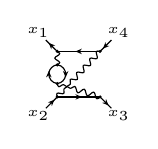
\begin{tikzpicture}[x=0.340cm, y=0.340cm, line width=0.420pt, baseline={([yshift=-0.6ex]0,0)}]
  \draw (1.067,0.850) -- (-0.533,0.850);
  \fill (0.147,0.850) -- (0.386,0.748) -- (0.308,0.850) -- (0.386,0.952) -- cycle;
  \draw (-0.533,-0.850) -- (1.067,-0.850);
  \fill (0.386,-0.850) -- (0.147,-0.748) -- (0.225,-0.850) -- (0.147,-0.952) -- cycle;
  \draw (-0.533,-0.350) arc[start angle=263.974, end angle=96.026, radius=0.352];
  \fill (-0.848,0.119) -- (-0.950,-0.119) -- (-0.848,-0.042) -- (-0.746,-0.119) -- cycle;
  \draw (-0.533,0.350) arc[start angle=83.974, end angle=-83.974, radius=0.352];
  \fill (-0.218,-0.119) -- (-0.116,0.119) -- (-0.218,0.042) -- (-0.320,0.119) -- cycle;
  \draw plot[smooth, tension=0.7] coordinates {(-0.533,0.850) (-0.470,0.808) (-0.443,0.767) (-0.470,0.725) (-0.533,0.683) (-0.597,0.642) (-0.623,0.600) (-0.597,0.558) (-0.533,0.517) (-0.470,0.475) (-0.443,0.433) (-0.470,0.392) (-0.533,0.350)};
  \draw plot[smooth, tension=0.7] coordinates {(-0.533,-0.850) (-0.552,-0.770) (-0.542,-0.718) (-0.491,-0.705) (-0.410,-0.719) (-0.330,-0.733) (-0.285,-0.714) (-0.281,-0.656) (-0.287,-0.588) (-0.273,-0.540) (-0.237,-0.513) (-0.197,-0.489) (-0.164,-0.458) (-0.130,-0.428) (-0.087,-0.407) (-0.051,-0.379) (-0.041,-0.327) (-0.051,-0.256) (-0.046,-0.199) (0.001,-0.182) (0.082,-0.196) (0.163,-0.210) (0.214,-0.197) (0.224,-0.145) (0.205,-0.065) (0.186,0.014) (0.196,0.066) (0.248,0.080) (0.328,0.065) (0.409,0.051) (0.460,0.064) (0.470,0.116) (0.451,0.196) (0.432,0.276) (0.442,0.328) (0.494,0.341) (0.574,0.327) (0.655,0.313) (0.707,0.326) (0.717,0.378) (0.697,0.458) (0.678,0.537) (0.688,0.590) (0.740,0.603) (0.821,0.588) (0.901,0.574) (0.953,0.587) (0.963,0.640) (0.944,0.719) (0.924,0.799) (0.935,0.851) (0.986,0.864) (1.067,0.850)};
  \draw plot[smooth, tension=0.7] coordinates {(1.067,-0.850) (1.001,-0.904) (0.948,-0.918) (0.912,-0.876) (0.889,-0.794) (0.866,-0.713) (0.830,-0.671) (0.777,-0.685) (0.711,-0.739) (0.645,-0.793) (0.592,-0.807) (0.557,-0.765) (0.533,-0.683) (0.510,-0.602) (0.474,-0.560) (0.421,-0.574) (0.356,-0.628) (0.290,-0.682) (0.237,-0.696) (0.201,-0.654) (0.178,-0.572) (0.154,-0.491) (0.116,-0.458) (0.060,-0.480) (0.000,-0.517) (-0.052,-0.526) (-0.094,-0.504) (-0.134,-0.477) (-0.178,-0.461) (-0.221,-0.442) (-0.260,-0.412) (-0.302,-0.391) (-0.356,-0.406) (-0.417,-0.447) (-0.473,-0.469) (-0.510,-0.432) (-0.533,-0.350)};
  \draw (-0.533,0.850) -- (-0.958,1.274);
  \fill (-0.851,1.168) -- (-0.754,0.927) -- (-0.737,1.054) -- (-0.610,1.071) -- cycle;
  \draw (-0.533,-0.850) -- (-0.958,-1.274);
  \fill (-0.640,-0.956) -- (-0.881,-1.053) -- (-0.754,-1.070) -- (-0.737,-1.197) -- cycle;
  \draw (1.067,-0.850) -- (1.491,-1.274);
  \fill (1.384,-1.168) -- (1.288,-0.927) -- (1.270,-1.054) -- (1.143,-1.071) -- cycle;
  \draw (1.067,0.850) -- (1.491,1.274);
  \fill (1.173,0.956) -- (1.414,1.053) -- (1.287,1.070) -- (1.270,1.197) -- cycle;
  \fill (-0.533,0.850) circle (0.064);
  \fill (-0.533,-0.850) circle (0.064);
  \fill (1.067,-0.850) circle (0.064);
  \fill (1.067,0.850) circle (0.064);
  \fill (-0.533,0.350) circle (0.064);
  \fill (-0.533,-0.350) circle (0.064);
  \node[font=\tiny, inner sep=0pt, anchor=315] at (-1.021,1.338) {$x_{1}$};
  \node[font=\tiny, inner sep=0pt, anchor=45] at (-1.021,-1.338) {$x_{2}$};
  \node[font=\tiny, inner sep=0pt, anchor=135] at (1.555,-1.338) {$x_{3}$};
  \node[font=\tiny, inner sep=0pt, anchor=225] at (1.555,1.338) {$x_{4}$};
\end{tikzpicture}}
\diagramgap
\mbox{$\displaystyle +\,$\,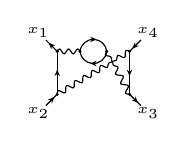
\begin{tikzpicture}[x=0.340cm, y=0.340cm, line width=0.420pt, baseline={([yshift=-0.6ex]0,0)}]
  \draw (-1.350,-1.067) -- (-1.350,0.533);
  \fill (-1.350,-0.147) -- (-1.452,-0.386) -- (-1.350,-0.308) -- (-1.248,-0.386) -- cycle;
  \draw (1.350,0.533) -- (1.350,-1.067);
  \fill (1.350,-0.386) -- (1.452,-0.147) -- (1.350,-0.225) -- (1.248,-0.147) -- cycle;
  \draw (0.500,0.533) arc[start angle=353.974, end angle=186.026, radius=0.503];
  \fill (-0.119,0.083) -- (0.119,-0.019) -- (0.042,0.083) -- (0.119,0.185) -- cycle;
  \draw (-0.500,0.533) arc[start angle=173.974, end angle=6.026, radius=0.503];
  \fill (0.119,0.983) -- (-0.119,1.085) -- (-0.042,0.983) -- (-0.119,0.881) -- cycle;
  \draw plot[smooth, tension=0.7] coordinates {(-1.350,0.533) (-1.308,0.598) (-1.265,0.625) (-1.223,0.598) (-1.180,0.533) (-1.138,0.468) (-1.095,0.442) (-1.052,0.468) (-1.010,0.533) (-0.968,0.598) (-0.925,0.625) (-0.883,0.598) (-0.840,0.533) (-0.798,0.468) (-0.755,0.442) (-0.713,0.468) (-0.670,0.533) (-0.628,0.598) (-0.585,0.625) (-0.543,0.598) (-0.500,0.533)};
  \draw plot[smooth, tension=0.7] coordinates {(-1.350,-1.067) (-1.346,-0.982) (-1.321,-0.934) (-1.267,-0.935) (-1.191,-0.973) (-1.116,-1.010) (-1.061,-1.011) (-1.036,-0.963) (-1.032,-0.878) (-1.029,-0.794) (-1.004,-0.746) (-0.949,-0.747) (-0.874,-0.784) (-0.798,-0.821) (-0.743,-0.823) (-0.718,-0.774) (-0.715,-0.690) (-0.711,-0.606) (-0.686,-0.557) (-0.632,-0.559) (-0.556,-0.596) (-0.480,-0.633) (-0.426,-0.635) (-0.401,-0.586) (-0.397,-0.502) (-0.393,-0.418) (-0.368,-0.369) (-0.314,-0.371) (-0.238,-0.408) (-0.163,-0.445) (-0.108,-0.447) (-0.083,-0.398) (-0.079,-0.314) (-0.076,-0.230) (-0.051,-0.181) (0.004,-0.182) (0.079,-0.220) (0.155,-0.257) (0.210,-0.258) (0.234,-0.210) (0.238,-0.125) (0.242,-0.041) (0.267,0.007) (0.321,0.006) (0.397,-0.031) (0.472,-0.068) (0.522,-0.061) (0.542,-0.005) (0.556,0.063) (0.584,0.106) (0.628,0.122) (0.674,0.135) (0.715,0.157) (0.757,0.175) (0.806,0.184) (0.849,0.201) (0.874,0.251) (0.884,0.325) (0.904,0.380) (0.957,0.382) (1.032,0.345) (1.108,0.308) (1.163,0.306) (1.187,0.355) (1.191,0.439) (1.195,0.523) (1.220,0.572) (1.274,0.570) (1.350,0.533)};
  \draw plot[smooth, tension=0.7] coordinates {(1.350,-1.067) (1.259,-1.058) (1.207,-1.029) (1.211,-0.969) (1.256,-0.889) (1.300,-0.808) (1.304,-0.749) (1.253,-0.719) (1.161,-0.711) (1.070,-0.703) (1.018,-0.673) (1.022,-0.614) (1.067,-0.533) (1.111,-0.453) (1.115,-0.393) (1.064,-0.364) (0.972,-0.356) (0.881,-0.347) (0.829,-0.318) (0.834,-0.258) (0.878,-0.178) (0.920,-0.099) (0.911,-0.046) (0.852,-0.021) (0.783,0.000) (0.742,0.035) (0.727,0.084) (0.712,0.133) (0.689,0.178) (0.674,0.227) (0.671,0.282) (0.652,0.329) (0.594,0.356) (0.511,0.368) (0.453,0.394) (0.456,0.453) (0.500,0.533)};
  \draw (-1.350,0.533) -- (-1.774,0.958);
  \fill (-1.668,0.851) -- (-1.571,0.610) -- (-1.554,0.737) -- (-1.427,0.754) -- cycle;
  \draw (-1.350,-1.067) -- (-1.774,-1.491);
  \fill (-1.456,-1.173) -- (-1.697,-1.270) -- (-1.570,-1.287) -- (-1.553,-1.414) -- cycle;
  \draw (1.350,-1.067) -- (1.774,-1.491);
  \fill (1.668,-1.384) -- (1.571,-1.143) -- (1.554,-1.270) -- (1.427,-1.288) -- cycle;
  \draw (1.350,0.533) -- (1.774,0.958);
  \fill (1.456,0.640) -- (1.697,0.737) -- (1.570,0.754) -- (1.553,0.881) -- cycle;
  \fill (-1.350,0.533) circle (0.064);
  \fill (-1.350,-1.067) circle (0.064);
  \fill (1.350,-1.067) circle (0.064);
  \fill (1.350,0.533) circle (0.064);
  \fill (-0.500,0.533) circle (0.064);
  \fill (0.500,0.533) circle (0.064);
  \node[font=\tiny, inner sep=0pt, anchor=315] at (-1.838,1.021) {$x_{1}$};
  \node[font=\tiny, inner sep=0pt, anchor=45] at (-1.838,-1.555) {$x_{2}$};
  \node[font=\tiny, inner sep=0pt, anchor=135] at (1.838,-1.555) {$x_{3}$};
  \node[font=\tiny, inner sep=0pt, anchor=225] at (1.838,1.021) {$x_{4}$};
\end{tikzpicture}}
\diagramgap
\mbox{$\displaystyle +\,$\,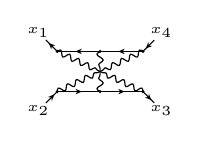
\begin{tikzpicture}[x=0.340cm, y=0.340cm, line width=0.420pt, baseline={([yshift=-0.6ex]0,0)}]
  \draw (0.000,0.750) -- (-1.600,0.750);
  \fill (-0.919,0.750) -- (-0.681,0.648) -- (-0.758,0.750) -- (-0.681,0.852) -- cycle;
  \draw (0.000,-0.750) -- (1.600,-0.750);
  \fill (0.919,-0.750) -- (0.681,-0.648) -- (0.758,-0.750) -- (0.681,-0.852) -- cycle;
  \draw (-1.600,-0.750) -- (0.000,-0.750);
  \fill (-0.681,-0.750) -- (-0.919,-0.648) -- (-0.842,-0.750) -- (-0.919,-0.852) -- cycle;
  \draw (1.600,0.750) -- (0.000,0.750);
  \fill (0.681,0.750) -- (0.919,0.648) -- (0.842,0.750) -- (0.919,0.852) -- cycle;
  \draw plot[smooth, tension=0.7] coordinates {(-1.600,0.750) (-1.528,0.795) (-1.473,0.801) (-1.444,0.755) (-1.432,0.671) (-1.420,0.587) (-1.390,0.541) (-1.335,0.548) (-1.263,0.592) (-1.191,0.637) (-1.136,0.644) (-1.107,0.597) (-1.095,0.513) (-1.083,0.429) (-1.053,0.383) (-0.999,0.390) (-0.926,0.434) (-0.854,0.479) (-0.799,0.486) (-0.770,0.439) (-0.758,0.355) (-0.746,0.271) (-0.716,0.225) (-0.662,0.232) (-0.589,0.276) (-0.517,0.321) (-0.463,0.328) (-0.433,0.281) (-0.421,0.197) (-0.409,0.113) (-0.379,0.067) (-0.325,0.074) (-0.253,0.118) (-0.192,0.138) (-0.154,0.110) (-0.122,0.068) (-0.084,0.039) (-0.042,0.020) (0.000,0.000) (0.042,-0.020) (0.084,-0.039) (0.131,-0.050) (0.183,-0.048) (0.229,-0.060) (0.253,-0.118) (0.265,-0.202) (0.294,-0.249) (0.349,-0.242) (0.421,-0.197) (0.493,-0.153) (0.548,-0.146) (0.578,-0.192) (0.589,-0.276) (0.601,-0.360) (0.631,-0.407) (0.686,-0.400) (0.758,-0.355) (0.830,-0.311) (0.885,-0.304) (0.914,-0.350) (0.926,-0.434) (0.938,-0.518) (0.968,-0.565) (1.022,-0.558) (1.095,-0.513) (1.167,-0.469) (1.222,-0.462) (1.251,-0.508) (1.263,-0.592) (1.275,-0.676) (1.305,-0.723) (1.359,-0.716) (1.432,-0.671) (1.504,-0.626) (1.558,-0.620) (1.588,-0.666) (1.600,-0.750)};
  \draw plot[smooth, tension=0.7] coordinates {(-1.600,-0.750) (-1.588,-0.666) (-1.558,-0.620) (-1.504,-0.626) (-1.432,-0.671) (-1.359,-0.716) (-1.305,-0.723) (-1.275,-0.676) (-1.263,-0.592) (-1.251,-0.508) (-1.222,-0.462) (-1.167,-0.469) (-1.095,-0.513) (-1.022,-0.558) (-0.968,-0.565) (-0.938,-0.518) (-0.926,-0.434) (-0.914,-0.350) (-0.885,-0.304) (-0.830,-0.311) (-0.758,-0.355) (-0.686,-0.400) (-0.631,-0.407) (-0.601,-0.360) (-0.589,-0.276) (-0.578,-0.192) (-0.548,-0.146) (-0.493,-0.153) (-0.421,-0.197) (-0.349,-0.242) (-0.294,-0.249) (-0.265,-0.202) (-0.253,-0.118) (-0.229,-0.060) (-0.183,-0.048) (-0.131,-0.050) (-0.084,-0.039) (-0.042,-0.020) (0.000,0.000) (0.042,0.020) (0.084,0.039) (0.122,0.068) (0.154,0.110) (0.192,0.138) (0.253,0.118) (0.325,0.074) (0.379,0.067) (0.409,0.113) (0.421,0.197) (0.433,0.281) (0.463,0.328) (0.517,0.321) (0.589,0.276) (0.662,0.232) (0.716,0.225) (0.746,0.271) (0.758,0.355) (0.770,0.439) (0.799,0.486) (0.854,0.479) (0.926,0.434) (0.999,0.390) (1.053,0.383) (1.083,0.429) (1.095,0.513) (1.107,0.597) (1.136,0.644) (1.191,0.637) (1.263,0.592) (1.335,0.548) (1.390,0.541) (1.420,0.587) (1.432,0.671) (1.444,0.755) (1.473,0.801) (1.528,0.795) (1.600,0.750)};
  \draw plot[smooth, tension=0.7] coordinates {(0.000,-0.750) (-0.082,-0.696) (-0.116,-0.643) (-0.082,-0.589) (0.000,-0.536) (0.082,-0.482) (0.116,-0.429) (0.081,-0.375) (0.000,-0.321) (-0.049,-0.268) (-0.039,-0.214) (-0.012,-0.161) (0.000,-0.107) (0.000,-0.054) (0.000,0.000) (0.000,0.054) (0.000,0.107) (-0.012,0.161) (-0.039,0.214) (-0.049,0.268) (0.000,0.321) (0.081,0.375) (0.116,0.429) (0.082,0.482) (0.000,0.536) (-0.082,0.589) (-0.116,0.643) (-0.082,0.696) (0.000,0.750)};
  \draw (-1.600,0.750) -- (-2.024,1.174);
  \fill (-1.918,1.068) -- (-1.821,0.827) -- (-1.804,0.954) -- (-1.677,0.971) -- cycle;
  \draw (-1.600,-0.750) -- (-2.024,-1.174);
  \fill (-1.706,-0.856) -- (-1.947,-0.953) -- (-1.820,-0.970) -- (-1.803,-1.097) -- cycle;
  \draw (1.600,-0.750) -- (2.024,-1.174);
  \fill (1.918,-1.068) -- (1.821,-0.827) -- (1.804,-0.954) -- (1.677,-0.971) -- cycle;
  \draw (1.600,0.750) -- (2.024,1.174);
  \fill (1.706,0.856) -- (1.947,0.953) -- (1.820,0.970) -- (1.803,1.097) -- cycle;
  \fill (-1.600,0.750) circle (0.064);
  \fill (-1.600,-0.750) circle (0.064);
  \fill (1.600,-0.750) circle (0.064);
  \fill (1.600,0.750) circle (0.064);
  \fill (0.000,-0.750) circle (0.064);
  \fill (0.000,0.750) circle (0.064);
  \node[font=\tiny, inner sep=0pt, anchor=315] at (-2.088,1.238) {$x_{1}$};
  \node[font=\tiny, inner sep=0pt, anchor=45] at (-2.088,-1.238) {$x_{2}$};
  \node[font=\tiny, inner sep=0pt, anchor=135] at (2.088,-1.238) {$x_{3}$};
  \node[font=\tiny, inner sep=0pt, anchor=225] at (2.088,1.238) {$x_{4}$};
\end{tikzpicture}}
\diagramgap
\mbox{$\displaystyle -\,$\,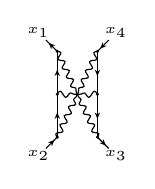
\begin{tikzpicture}[x=0.340cm, y=0.340cm, line width=0.420pt, baseline={([yshift=-0.6ex]0,0)}]
  \draw (-0.750,0.000) -- (-0.750,1.600);
  \fill (-0.750,0.919) -- (-0.852,0.681) -- (-0.750,0.758) -- (-0.648,0.681) -- cycle;
  \draw (0.750,0.000) -- (0.750,-1.600);
  \fill (0.750,-0.919) -- (0.852,-0.681) -- (0.750,-0.758) -- (0.648,-0.681) -- cycle;
  \draw (-0.750,-1.600) -- (-0.750,0.000);
  \fill (-0.750,-0.681) -- (-0.852,-0.919) -- (-0.750,-0.842) -- (-0.648,-0.919) -- cycle;
  \draw (0.750,1.600) -- (0.750,0.000);
  \fill (0.750,0.681) -- (0.852,0.919) -- (0.750,0.842) -- (0.648,0.919) -- cycle;
  \draw plot[smooth, tension=0.7] coordinates {(-0.750,1.600) (-0.666,1.588) (-0.620,1.558) (-0.626,1.504) (-0.671,1.432) (-0.716,1.359) (-0.723,1.305) (-0.676,1.275) (-0.592,1.263) (-0.508,1.251) (-0.462,1.222) (-0.469,1.167) (-0.513,1.095) (-0.558,1.022) (-0.565,0.968) (-0.518,0.938) (-0.434,0.926) (-0.350,0.914) (-0.304,0.885) (-0.311,0.830) (-0.355,0.758) (-0.400,0.686) (-0.407,0.631) (-0.360,0.601) (-0.276,0.589) (-0.192,0.578) (-0.146,0.548) (-0.153,0.493) (-0.197,0.421) (-0.242,0.349) (-0.249,0.294) (-0.202,0.265) (-0.118,0.253) (-0.060,0.229) (-0.048,0.183) (-0.050,0.131) (-0.039,0.084) (-0.020,0.042) (0.000,0.000) (0.020,-0.042) (0.039,-0.084) (0.068,-0.122) (0.110,-0.154) (0.138,-0.192) (0.118,-0.253) (0.074,-0.325) (0.067,-0.379) (0.113,-0.409) (0.197,-0.421) (0.281,-0.433) (0.328,-0.463) (0.321,-0.517) (0.276,-0.589) (0.232,-0.662) (0.225,-0.716) (0.271,-0.746) (0.355,-0.758) (0.439,-0.770) (0.486,-0.799) (0.479,-0.854) (0.434,-0.926) (0.390,-0.999) (0.383,-1.053) (0.429,-1.083) (0.513,-1.095) (0.597,-1.107) (0.644,-1.136) (0.637,-1.191) (0.592,-1.263) (0.548,-1.335) (0.541,-1.390) (0.587,-1.420) (0.671,-1.432) (0.755,-1.444) (0.801,-1.473) (0.795,-1.528) (0.750,-1.600)};
  \draw plot[smooth, tension=0.7] coordinates {(-0.750,-1.600) (-0.795,-1.528) (-0.801,-1.473) (-0.755,-1.444) (-0.671,-1.432) (-0.587,-1.420) (-0.541,-1.390) (-0.548,-1.335) (-0.592,-1.263) (-0.637,-1.191) (-0.644,-1.136) (-0.597,-1.107) (-0.513,-1.095) (-0.429,-1.083) (-0.383,-1.053) (-0.390,-0.999) (-0.434,-0.926) (-0.479,-0.854) (-0.486,-0.799) (-0.439,-0.770) (-0.355,-0.758) (-0.271,-0.746) (-0.225,-0.716) (-0.232,-0.662) (-0.276,-0.589) (-0.321,-0.517) (-0.328,-0.463) (-0.281,-0.433) (-0.197,-0.421) (-0.113,-0.409) (-0.067,-0.379) (-0.074,-0.325) (-0.118,-0.253) (-0.138,-0.192) (-0.110,-0.154) (-0.068,-0.122) (-0.039,-0.084) (-0.020,-0.042) (0.000,0.000) (0.020,0.042) (0.039,0.084) (0.050,0.131) (0.048,0.183) (0.060,0.229) (0.118,0.253) (0.202,0.265) (0.249,0.294) (0.242,0.349) (0.197,0.421) (0.153,0.493) (0.146,0.548) (0.192,0.578) (0.276,0.589) (0.360,0.601) (0.407,0.631) (0.400,0.686) (0.355,0.758) (0.311,0.830) (0.304,0.885) (0.350,0.914) (0.434,0.926) (0.518,0.938) (0.565,0.968) (0.558,1.022) (0.513,1.095) (0.469,1.167) (0.462,1.222) (0.508,1.251) (0.592,1.263) (0.676,1.275) (0.723,1.305) (0.716,1.359) (0.671,1.432) (0.626,1.504) (0.620,1.558) (0.666,1.588) (0.750,1.600)};
  \draw plot[smooth, tension=0.7] coordinates {(-0.750,0.000) (-0.696,0.082) (-0.643,0.116) (-0.589,0.082) (-0.536,0.000) (-0.482,-0.082) (-0.429,-0.116) (-0.375,-0.081) (-0.321,0.000) (-0.268,0.049) (-0.214,0.039) (-0.161,0.012) (-0.107,0.000) (-0.054,0.000) (0.000,0.000) (0.054,0.000) (0.107,0.000) (0.161,0.012) (0.214,0.039) (0.268,0.049) (0.321,0.000) (0.375,-0.081) (0.429,-0.116) (0.482,-0.082) (0.536,0.000) (0.589,0.082) (0.643,0.116) (0.696,0.082) (0.750,0.000)};
  \draw (-0.750,1.600) -- (-1.174,2.024);
  \fill (-1.068,1.918) -- (-0.971,1.677) -- (-0.954,1.804) -- (-0.827,1.821) -- cycle;
  \draw (-0.750,-1.600) -- (-1.174,-2.024);
  \fill (-0.856,-1.706) -- (-1.097,-1.803) -- (-0.970,-1.820) -- (-0.953,-1.947) -- cycle;
  \draw (0.750,-1.600) -- (1.174,-2.024);
  \fill (1.068,-1.918) -- (0.971,-1.677) -- (0.954,-1.804) -- (0.827,-1.821) -- cycle;
  \draw (0.750,1.600) -- (1.174,2.024);
  \fill (0.856,1.706) -- (1.097,1.803) -- (0.970,1.820) -- (0.953,1.947) -- cycle;
  \fill (-0.750,1.600) circle (0.064);
  \fill (-0.750,-1.600) circle (0.064);
  \fill (0.750,-1.600) circle (0.064);
  \fill (0.750,1.600) circle (0.064);
  \fill (-0.750,0.000) circle (0.064);
  \fill (0.750,0.000) circle (0.064);
  \node[font=\tiny, inner sep=0pt, anchor=315] at (-1.238,2.088) {$x_{1}$};
  \node[font=\tiny, inner sep=0pt, anchor=45] at (-1.238,-2.088) {$x_{2}$};
  \node[font=\tiny, inner sep=0pt, anchor=135] at (1.238,-2.088) {$x_{3}$};
  \node[font=\tiny, inner sep=0pt, anchor=225] at (1.238,2.088) {$x_{4}$};
\end{tikzpicture}}
\diagramgap
\mbox{$\displaystyle +\,$\,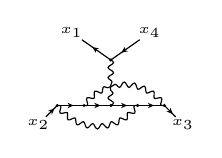
\begin{tikzpicture}[x=0.340cm, y=0.340cm, line width=0.420pt, baseline={([yshift=-0.6ex]0,0)}]
  \draw (1.000,-0.283) -- (2.000,-0.283);
  \fill (1.619,-0.283) -- (1.381,-0.181) -- (1.458,-0.283) -- (1.381,-0.385) -- cycle;
  \draw (-2.000,-0.283) -- (-1.000,-0.283);
  \fill (-1.381,-0.283) -- (-1.619,-0.181) -- (-1.542,-0.283) -- (-1.619,-0.385) -- cycle;
  \draw (0.000,-0.283) -- (1.000,-0.283);
  \fill (0.619,-0.283) -- (0.381,-0.181) -- (0.458,-0.283) -- (0.381,-0.385) -- cycle;
  \draw (-1.000,-0.283) -- (0.000,-0.283);
  \fill (-0.381,-0.283) -- (-0.619,-0.181) -- (-0.542,-0.283) -- (-0.619,-0.385) -- cycle;
  \draw plot[smooth, tension=0.7] coordinates {(0.000,1.417) (0.072,1.369) (0.102,1.322) (0.072,1.275) (0.000,1.228) (-0.072,1.181) (-0.102,1.133) (-0.072,1.086) (0.000,1.039) (0.072,0.992) (0.102,0.944) (0.072,0.897) (0.000,0.850) (-0.072,0.803) (-0.102,0.756) (-0.067,0.708) (0.000,0.661) (0.042,0.614) (0.038,0.567) (0.013,0.519) (0.000,0.472) (0.000,0.425) (-0.006,0.378) (-0.014,0.331) (0.000,0.283) (0.042,0.236) (0.080,0.189) (0.067,0.142) (0.000,0.094) (-0.072,0.047) (-0.102,0.000) (-0.072,-0.047) (0.000,-0.094) (0.072,-0.142) (0.102,-0.189) (0.072,-0.236) (0.000,-0.283)};
  \draw plot[smooth, tension=0.7] coordinates {(-2.000,-0.283) (-1.918,-0.280) (-1.869,-0.299) (-1.864,-0.351) (-1.886,-0.429) (-1.906,-0.510) (-1.894,-0.564) (-1.840,-0.579) (-1.759,-0.563) (-1.679,-0.543) (-1.627,-0.551) (-1.611,-0.601) (-1.618,-0.683) (-1.621,-0.765) (-1.598,-0.816) (-1.542,-0.820) (-1.466,-0.788) (-1.392,-0.753) (-1.340,-0.751) (-1.314,-0.796) (-1.304,-0.877) (-1.291,-0.959) (-1.258,-1.004) (-1.202,-0.997) (-1.134,-0.950) (-1.069,-0.901) (-1.018,-0.888) (-0.984,-0.928) (-0.958,-1.005) (-0.928,-1.083) (-0.887,-1.120) (-0.834,-1.102) (-0.776,-1.042) (-0.722,-0.981) (-0.675,-0.958) (-0.633,-0.990) (-0.592,-1.061) (-0.548,-1.131) (-0.500,-1.160) (-0.452,-1.131) (-0.408,-1.061) (-0.367,-0.990) (-0.325,-0.958) (-0.278,-0.981) (-0.224,-1.042) (-0.166,-1.102) (-0.113,-1.120) (-0.072,-1.083) (-0.042,-1.005) (-0.016,-0.928) (0.018,-0.888) (0.069,-0.901) (0.134,-0.950) (0.202,-0.997) (0.258,-1.004) (0.291,-0.959) (0.304,-0.877) (0.314,-0.796) (0.340,-0.751) (0.392,-0.753) (0.466,-0.788) (0.542,-0.820) (0.598,-0.816) (0.621,-0.765) (0.618,-0.683) (0.611,-0.601) (0.627,-0.551) (0.679,-0.543) (0.759,-0.563) (0.840,-0.579) (0.894,-0.564) (0.906,-0.510) (0.886,-0.429) (0.864,-0.351) (0.869,-0.299) (0.918,-0.280) (1.000,-0.283)};
  \draw plot[smooth, tension=0.7] coordinates {(2.000,-0.283) (1.918,-0.286) (1.869,-0.268) (1.864,-0.216) (1.886,-0.138) (1.906,-0.057) (1.894,-0.003) (1.840,0.012) (1.759,-0.004) (1.679,-0.023) (1.627,-0.015) (1.611,0.035) (1.618,0.116) (1.621,0.199) (1.598,0.250) (1.542,0.253) (1.466,0.221) (1.392,0.187) (1.340,0.184) (1.314,0.230) (1.304,0.311) (1.291,0.392) (1.258,0.438) (1.202,0.430) (1.134,0.383) (1.069,0.335) (1.018,0.321) (0.984,0.361) (0.958,0.439) (0.928,0.516) (0.887,0.554) (0.834,0.535) (0.776,0.476) (0.722,0.415) (0.675,0.392) (0.633,0.424) (0.592,0.494) (0.548,0.564) (0.500,0.593) (0.452,0.564) (0.408,0.494) (0.367,0.424) (0.325,0.392) (0.277,0.420) (0.224,0.476) (0.171,0.507) (0.125,0.494) (0.085,0.462) (0.042,0.439) (-0.002,0.427) (-0.045,0.408) (-0.086,0.386) (-0.134,0.383) (-0.192,0.404) (-0.250,0.419) (-0.289,0.388) (-0.304,0.311) (-0.314,0.230) (-0.340,0.184) (-0.392,0.187) (-0.466,0.221) (-0.542,0.253) (-0.598,0.250) (-0.621,0.199) (-0.618,0.116) (-0.611,0.035) (-0.627,-0.015) (-0.679,-0.023) (-0.759,-0.004) (-0.840,0.012) (-0.894,-0.003) (-0.906,-0.057) (-0.886,-0.138) (-0.864,-0.216) (-0.869,-0.268) (-0.918,-0.286) (-1.000,-0.283)};
  \draw (0.000,1.417) -- (-1.081,2.174);
  \fill (-0.693,1.902) -- (-0.555,1.681) -- (-0.560,1.809) -- (-0.438,1.848) -- cycle;
  \draw (-2.000,-0.283) -- (-2.424,-0.708);
  \fill (-2.106,-0.390) -- (-2.347,-0.487) -- (-2.220,-0.504) -- (-2.203,-0.631) -- cycle;
  \draw (2.000,-0.283) -- (2.424,-0.708);
  \fill (2.318,-0.601) -- (2.221,-0.360) -- (2.204,-0.487) -- (2.077,-0.504) -- cycle;
  \draw (0.000,1.417) -- (1.081,2.174);
  \fill (0.389,1.689) -- (0.643,1.742) -- (0.521,1.781) -- (0.526,1.909) -- cycle;
  \fill (0.000,1.417) circle (0.064);
  \fill (-2.000,-0.283) circle (0.064);
  \fill (2.000,-0.283) circle (0.064);
  \fill (-1.000,-0.283) circle (0.064);
  \fill (1.000,-0.283) circle (0.064);
  \fill (0.000,-0.283) circle (0.064);
  \node[font=\tiny, inner sep=0pt, anchor=325] at (-1.155,2.225) {$x_{1}$};
  \node[font=\tiny, inner sep=0pt, anchor=45] at (-2.488,-0.771) {$x_{2}$};
  \node[font=\tiny, inner sep=0pt, anchor=135] at (2.488,-0.771) {$x_{3}$};
  \node[font=\tiny, inner sep=0pt, anchor=215] at (1.155,2.225) {$x_{4}$};
\end{tikzpicture}}
\diagramgap
\mbox{$\displaystyle +\,$\,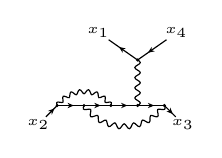
\begin{tikzpicture}[x=0.340cm, y=0.340cm, line width=0.420pt, baseline={([yshift=-0.6ex]0,0)}]
  \draw (0.833,-0.283) -- (1.833,-0.283);
  \fill (1.453,-0.283) -- (1.214,-0.181) -- (1.292,-0.283) -- (1.214,-0.385) -- cycle;
  \draw (-2.167,-0.283) -- (-1.167,-0.283);
  \fill (-1.547,-0.283) -- (-1.786,-0.181) -- (-1.708,-0.283) -- (-1.786,-0.385) -- cycle;
  \draw (-0.167,-0.283) -- (0.833,-0.283);
  \fill (0.453,-0.283) -- (0.214,-0.181) -- (0.292,-0.283) -- (0.214,-0.385) -- cycle;
  \draw (-1.167,-0.283) -- (-0.167,-0.283);
  \fill (-0.547,-0.283) -- (-0.786,-0.181) -- (-0.708,-0.283) -- (-0.786,-0.385) -- cycle;
  \draw plot[smooth, tension=0.7] coordinates {(0.833,1.417) (0.905,1.369) (0.935,1.322) (0.905,1.275) (0.833,1.228) (0.761,1.181) (0.731,1.133) (0.761,1.086) (0.833,1.039) (0.905,0.992) (0.935,0.944) (0.905,0.897) (0.833,0.850) (0.761,0.803) (0.731,0.756) (0.761,0.708) (0.833,0.661) (0.905,0.614) (0.935,0.567) (0.905,0.519) (0.833,0.472) (0.761,0.425) (0.731,0.378) (0.761,0.331) (0.833,0.283) (0.905,0.236) (0.935,0.189) (0.905,0.142) (0.833,0.094) (0.761,0.047) (0.731,0.000) (0.761,-0.047) (0.833,-0.094) (0.905,-0.142) (0.935,-0.189) (0.905,-0.236) (0.833,-0.283)};
  \draw plot[smooth, tension=0.7] coordinates {(-2.167,-0.283) (-2.190,-0.217) (-2.183,-0.170) (-2.139,-0.153) (-2.069,-0.162) (-2.001,-0.173) (-1.958,-0.164) (-1.948,-0.122) (-1.957,-0.053) (-1.962,0.017) (-1.944,0.061) (-1.897,0.065) (-1.831,0.040) (-1.769,0.012) (-1.725,0.010) (-1.704,0.048) (-1.695,0.116) (-1.683,0.185) (-1.654,0.223) (-1.607,0.216) (-1.551,0.175) (-1.497,0.131) (-1.455,0.118) (-1.425,0.150) (-1.400,0.214) (-1.370,0.278) (-1.333,0.307) (-1.289,0.288) (-1.245,0.234) (-1.204,0.179) (-1.167,0.155) (-1.129,0.179) (-1.089,0.234) (-1.044,0.288) (-1.001,0.307) (-0.963,0.278) (-0.934,0.214) (-0.908,0.150) (-0.878,0.118) (-0.836,0.131) (-0.783,0.175) (-0.726,0.216) (-0.679,0.223) (-0.650,0.185) (-0.638,0.116) (-0.630,0.048) (-0.609,0.010) (-0.565,0.012) (-0.502,0.040) (-0.437,0.065) (-0.389,0.061) (-0.371,0.017) (-0.377,-0.053) (-0.386,-0.122) (-0.375,-0.164) (-0.332,-0.173) (-0.264,-0.162) (-0.195,-0.153) (-0.150,-0.170) (-0.144,-0.217) (-0.167,-0.283)};
  \draw plot[smooth, tension=0.7] coordinates {(1.833,-0.283) (1.861,-0.361) (1.854,-0.417) (1.802,-0.437) (1.720,-0.429) (1.639,-0.418) (1.588,-0.431) (1.577,-0.482) (1.592,-0.563) (1.603,-0.645) (1.585,-0.698) (1.530,-0.707) (1.451,-0.683) (1.374,-0.656) (1.322,-0.658) (1.301,-0.706) (1.299,-0.788) (1.294,-0.871) (1.266,-0.919) (1.210,-0.917) (1.137,-0.877) (1.067,-0.835) (1.015,-0.828) (0.985,-0.870) (0.967,-0.950) (0.946,-1.030) (0.908,-1.072) (0.854,-1.059) (0.791,-1.005) (0.731,-0.950) (0.681,-0.932) (0.643,-0.968) (0.610,-1.042) (0.572,-1.116) (0.528,-1.150) (0.477,-1.126) (0.426,-1.061) (0.378,-0.995) (0.333,-0.967) (0.289,-0.995) (0.241,-1.061) (0.190,-1.126) (0.139,-1.150) (0.094,-1.116) (0.057,-1.042) (0.023,-0.968) (-0.015,-0.932) (-0.064,-0.950) (-0.124,-1.005) (-0.187,-1.059) (-0.242,-1.072) (-0.279,-1.030) (-0.301,-0.950) (-0.319,-0.870) (-0.349,-0.828) (-0.401,-0.835) (-0.471,-0.877) (-0.543,-0.917) (-0.599,-0.919) (-0.627,-0.871) (-0.633,-0.788) (-0.634,-0.706) (-0.655,-0.658) (-0.707,-0.656) (-0.785,-0.683) (-0.864,-0.707) (-0.919,-0.698) (-0.937,-0.645) (-0.925,-0.563) (-0.910,-0.482) (-0.921,-0.431) (-0.972,-0.418) (-1.053,-0.429) (-1.135,-0.437) (-1.188,-0.417) (-1.194,-0.361) (-1.167,-0.283)};
  \draw (0.833,1.417) -- (-0.248,2.174);
  \fill (0.141,1.902) -- (0.278,1.681) -- (0.273,1.809) -- (0.395,1.848) -- cycle;
  \draw (-2.167,-0.283) -- (-2.591,-0.708);
  \fill (-2.273,-0.390) -- (-2.514,-0.487) -- (-2.387,-0.504) -- (-2.370,-0.631) -- cycle;
  \draw (1.833,-0.283) -- (2.258,-0.708);
  \fill (2.151,-0.601) -- (2.054,-0.360) -- (2.037,-0.487) -- (1.910,-0.504) -- cycle;
  \draw (0.833,1.417) -- (1.915,2.174);
  \fill (1.222,1.689) -- (1.476,1.742) -- (1.354,1.781) -- (1.359,1.909) -- cycle;
  \fill (0.833,1.417) circle (0.064);
  \fill (-2.167,-0.283) circle (0.064);
  \fill (1.833,-0.283) circle (0.064);
  \fill (-1.167,-0.283) circle (0.064);
  \fill (0.833,-0.283) circle (0.064);
  \fill (-0.167,-0.283) circle (0.064);
  \node[font=\tiny, inner sep=0pt, anchor=325] at (-0.322,2.225) {$x_{1}$};
  \node[font=\tiny, inner sep=0pt, anchor=45] at (-2.655,-0.771) {$x_{2}$};
  \node[font=\tiny, inner sep=0pt, anchor=135] at (2.321,-0.771) {$x_{3}$};
  \node[font=\tiny, inner sep=0pt, anchor=215] at (1.988,2.225) {$x_{4}$};
\end{tikzpicture}}
\diagramgap
\mbox{$\displaystyle +\,$\,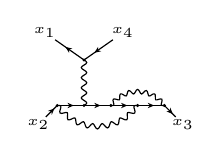
\begin{tikzpicture}[x=0.340cm, y=0.340cm, line width=0.420pt, baseline={([yshift=-0.6ex]0,0)}]
  \draw (1.167,-0.283) -- (2.167,-0.283);
  \fill (1.786,-0.283) -- (1.547,-0.181) -- (1.625,-0.283) -- (1.547,-0.385) -- cycle;
  \draw (-1.833,-0.283) -- (-0.833,-0.283);
  \fill (-1.214,-0.283) -- (-1.453,-0.181) -- (-1.375,-0.283) -- (-1.453,-0.385) -- cycle;
  \draw (0.167,-0.283) -- (1.167,-0.283);
  \fill (0.786,-0.283) -- (0.547,-0.181) -- (0.625,-0.283) -- (0.547,-0.385) -- cycle;
  \draw (-0.833,-0.283) -- (0.167,-0.283);
  \fill (-0.214,-0.283) -- (-0.453,-0.181) -- (-0.375,-0.283) -- (-0.453,-0.385) -- cycle;
  \draw plot[smooth, tension=0.7] coordinates {(-0.833,1.417) (-0.761,1.369) (-0.731,1.322) (-0.761,1.275) (-0.833,1.228) (-0.905,1.181) (-0.935,1.133) (-0.905,1.086) (-0.833,1.039) (-0.761,0.992) (-0.731,0.944) (-0.761,0.897) (-0.833,0.850) (-0.905,0.803) (-0.935,0.756) (-0.905,0.708) (-0.833,0.661) (-0.761,0.614) (-0.731,0.567) (-0.761,0.519) (-0.833,0.472) (-0.905,0.425) (-0.935,0.378) (-0.905,0.331) (-0.833,0.283) (-0.761,0.236) (-0.731,0.189) (-0.761,0.142) (-0.833,0.094) (-0.905,0.047) (-0.935,0.000) (-0.905,-0.047) (-0.833,-0.094) (-0.761,-0.142) (-0.731,-0.189) (-0.761,-0.236) (-0.833,-0.283)};
  \draw plot[smooth, tension=0.7] coordinates {(-1.833,-0.283) (-1.752,-0.280) (-1.702,-0.299) (-1.697,-0.351) (-1.720,-0.429) (-1.739,-0.510) (-1.727,-0.564) (-1.673,-0.579) (-1.592,-0.563) (-1.512,-0.543) (-1.461,-0.551) (-1.445,-0.601) (-1.451,-0.683) (-1.454,-0.765) (-1.431,-0.816) (-1.376,-0.820) (-1.299,-0.788) (-1.225,-0.753) (-1.173,-0.751) (-1.147,-0.796) (-1.137,-0.877) (-1.124,-0.959) (-1.091,-1.004) (-1.036,-0.997) (-0.967,-0.950) (-0.902,-0.901) (-0.851,-0.888) (-0.817,-0.928) (-0.791,-1.005) (-0.761,-1.083) (-0.720,-1.120) (-0.667,-1.102) (-0.610,-1.042) (-0.555,-0.981) (-0.508,-0.958) (-0.467,-0.990) (-0.426,-1.061) (-0.381,-1.131) (-0.333,-1.160) (-0.285,-1.131) (-0.241,-1.061) (-0.200,-0.990) (-0.158,-0.958) (-0.111,-0.981) (-0.057,-1.042) (0.001,-1.102) (0.053,-1.120) (0.095,-1.083) (0.124,-1.005) (0.150,-0.928) (0.184,-0.888) (0.235,-0.901) (0.301,-0.950) (0.369,-0.997) (0.424,-1.004) (0.457,-0.959) (0.471,-0.877) (0.481,-0.796) (0.506,-0.751) (0.559,-0.753) (0.633,-0.788) (0.709,-0.820) (0.765,-0.816) (0.788,-0.765) (0.785,-0.683) (0.778,-0.601) (0.794,-0.551) (0.846,-0.543) (0.925,-0.563) (1.006,-0.579) (1.060,-0.564) (1.073,-0.510) (1.053,-0.429) (1.030,-0.351) (1.036,-0.299) (1.085,-0.280) (1.167,-0.283)};
  \draw plot[smooth, tension=0.7] coordinates {(2.167,-0.283) (2.098,-0.286) (2.056,-0.272) (2.051,-0.228) (2.069,-0.162) (2.083,-0.093) (2.071,-0.047) (2.025,-0.036) (1.957,-0.053) (1.891,-0.073) (1.847,-0.070) (1.831,-0.029) (1.831,0.040) (1.828,0.110) (1.804,0.151) (1.757,0.150) (1.695,0.116) (1.637,0.080) (1.593,0.073) (1.568,0.108) (1.551,0.175) (1.530,0.242) (1.496,0.276) (1.450,0.262) (1.400,0.214) (1.352,0.164) (1.312,0.146) (1.278,0.174) (1.245,0.234) (1.208,0.293) (1.167,0.318) (1.126,0.293) (1.089,0.234) (1.055,0.174) (1.021,0.146) (0.981,0.164) (0.934,0.214) (0.883,0.262) (0.837,0.276) (0.804,0.242) (0.783,0.175) (0.766,0.108) (0.740,0.073) (0.697,0.080) (0.638,0.116) (0.577,0.150) (0.529,0.151) (0.505,0.110) (0.502,0.040) (0.502,-0.029) (0.486,-0.070) (0.443,-0.073) (0.377,-0.053) (0.309,-0.036) (0.262,-0.047) (0.250,-0.093) (0.264,-0.162) (0.282,-0.228) (0.277,-0.272) (0.236,-0.286) (0.167,-0.283)};
  \draw (-0.833,1.417) -- (-1.915,2.174);
  \fill (-1.526,1.902) -- (-1.389,1.681) -- (-1.394,1.809) -- (-1.272,1.848) -- cycle;
  \draw (-1.833,-0.283) -- (-2.258,-0.708);
  \fill (-1.940,-0.390) -- (-2.181,-0.487) -- (-2.054,-0.504) -- (-2.037,-0.631) -- cycle;
  \draw (2.167,-0.283) -- (2.591,-0.708);
  \fill (2.484,-0.601) -- (2.388,-0.360) -- (2.370,-0.487) -- (2.243,-0.504) -- cycle;
  \draw (-0.833,1.417) -- (0.248,2.174);
  \fill (-0.445,1.689) -- (-0.190,1.742) -- (-0.313,1.781) -- (-0.307,1.909) -- cycle;
  \fill (-0.833,1.417) circle (0.064);
  \fill (-1.833,-0.283) circle (0.064);
  \fill (2.167,-0.283) circle (0.064);
  \fill (-0.833,-0.283) circle (0.064);
  \fill (1.167,-0.283) circle (0.064);
  \fill (0.167,-0.283) circle (0.064);
  \node[font=\tiny, inner sep=0pt, anchor=325] at (-1.988,2.225) {$x_{1}$};
  \node[font=\tiny, inner sep=0pt, anchor=45] at (-2.321,-0.771) {$x_{2}$};
  \node[font=\tiny, inner sep=0pt, anchor=135] at (2.655,-0.771) {$x_{3}$};
  \node[font=\tiny, inner sep=0pt, anchor=215] at (0.322,2.225) {$x_{4}$};
\end{tikzpicture}}
\diagramgap
\mbox{$\displaystyle -\,$\,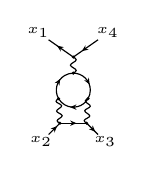
\begin{tikzpicture}[x=0.340cm, y=0.340cm, line width=0.420pt, baseline={([yshift=-0.6ex]0,0)}]
  \draw (-0.500,-1.029) -- (0.500,-1.029);
  \fill (0.119,-1.029) -- (-0.119,-0.927) -- (-0.042,-1.029) -- (-0.119,-1.131) -- cycle;
  \draw (-0.550,-0.112) arc[start angle=210.000, end angle=90.000, radius=0.635];
  \fill (-0.490,0.627) -- (-0.698,0.471) -- (-0.571,0.487) -- (-0.521,0.369) -- cycle;
  \draw (0.550,-0.112) arc[start angle=330.000, end angle=210.000, radius=0.635];
  \fill (-0.119,-0.429) -- (0.119,-0.531) -- (0.042,-0.429) -- (0.119,-0.327) -- cycle;
  \draw (0.000,0.841) arc[start angle=90.000, end angle=-30.000, radius=0.635];
  \fill (0.610,0.420) -- (0.579,0.678) -- (0.529,0.560) -- (0.402,0.576) -- cycle;
  \draw plot[smooth, tension=0.7] coordinates {(0.000,1.441) (0.076,1.391) (0.108,1.341) (0.076,1.291) (0.000,1.241) (-0.076,1.191) (-0.108,1.141) (-0.076,1.091) (0.000,1.041) (0.076,0.991) (0.108,0.941) (0.076,0.891) (0.000,0.841)};
  \draw plot[smooth, tension=0.7] coordinates {(-0.500,-1.029) (-0.573,-0.987) (-0.604,-0.943) (-0.578,-0.895) (-0.510,-0.846) (-0.442,-0.796) (-0.416,-0.749) (-0.447,-0.704) (-0.520,-0.662) (-0.593,-0.620) (-0.624,-0.576) (-0.598,-0.528) (-0.530,-0.479) (-0.462,-0.429) (-0.436,-0.382) (-0.467,-0.337) (-0.540,-0.295) (-0.613,-0.253) (-0.644,-0.209) (-0.618,-0.161) (-0.550,-0.112)};
  \draw plot[smooth, tension=0.7] coordinates {(0.500,-1.029) (0.432,-0.980) (0.406,-0.932) (0.437,-0.888) (0.510,-0.846) (0.583,-0.804) (0.614,-0.759) (0.588,-0.712) (0.520,-0.662) (0.452,-0.613) (0.426,-0.565) (0.457,-0.521) (0.530,-0.479) (0.603,-0.437) (0.634,-0.392) (0.608,-0.345) (0.540,-0.295) (0.472,-0.246) (0.446,-0.198) (0.477,-0.154) (0.550,-0.112)};
  \draw (0.000,1.441) -- (-0.924,2.088);
  \fill (-0.606,1.865) -- (-0.469,1.645) -- (-0.474,1.773) -- (-0.352,1.812) -- cycle;
  \draw (-0.500,-1.029) -- (-0.924,-1.454);
  \fill (-0.606,-1.136) -- (-0.847,-1.232) -- (-0.720,-1.250) -- (-0.703,-1.377) -- cycle;
  \draw (0.500,-1.029) -- (0.924,-1.454);
  \fill (0.818,-1.347) -- (0.721,-1.106) -- (0.704,-1.233) -- (0.577,-1.250) -- cycle;
  \draw (0.000,1.441) -- (0.924,2.088);
  \fill (0.318,1.664) -- (0.572,1.717) -- (0.450,1.756) -- (0.455,1.884) -- cycle;
  \fill (0.000,1.441) circle (0.064);
  \fill (-0.500,-1.029) circle (0.064);
  \fill (0.500,-1.029) circle (0.064);
  \fill (0.000,0.841) circle (0.064);
  \fill (-0.550,-0.112) circle (0.064);
  \fill (0.550,-0.112) circle (0.064);
  \node[font=\tiny, inner sep=0pt, anchor=325] at (-0.998,2.140) {$x_{1}$};
  \node[font=\tiny, inner sep=0pt, anchor=45] at (-0.988,-1.517) {$x_{2}$};
  \node[font=\tiny, inner sep=0pt, anchor=135] at (0.988,-1.517) {$x_{3}$};
  \node[font=\tiny, inner sep=0pt, anchor=215] at (0.998,2.140) {$x_{4}$};
\end{tikzpicture}}
\diagramgap
\mbox{$\displaystyle -\,$\,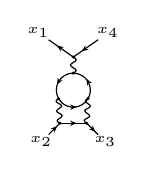
\begin{tikzpicture}[x=0.340cm, y=0.340cm, line width=0.420pt, baseline={([yshift=-0.6ex]0,0)}]
  \draw (-0.500,-1.029) -- (0.500,-1.029);
  \fill (0.119,-1.029) -- (-0.119,-0.927) -- (-0.042,-1.029) -- (-0.119,-1.131) -- cycle;
  \draw (0.550,-0.112) arc[start angle=330.000, end angle=450.000, radius=0.635];
  \fill (0.490,0.627) -- (0.521,0.369) -- (0.571,0.487) -- (0.698,0.471) -- cycle;
  \draw (0.000,0.841) arc[start angle=90.000, end angle=210.000, radius=0.635];
  \fill (-0.610,0.420) -- (-0.402,0.576) -- (-0.529,0.560) -- (-0.579,0.678) -- cycle;
  \draw (-0.550,-0.112) arc[start angle=210.000, end angle=330.000, radius=0.635];
  \fill (0.119,-0.429) -- (-0.119,-0.327) -- (-0.042,-0.429) -- (-0.119,-0.531) -- cycle;
  \draw plot[smooth, tension=0.7] coordinates {(0.000,1.441) (0.076,1.391) (0.108,1.341) (0.076,1.291) (0.000,1.241) (-0.076,1.191) (-0.108,1.141) (-0.076,1.091) (0.000,1.041) (0.076,0.991) (0.108,0.941) (0.076,0.891) (0.000,0.841)};
  \draw plot[smooth, tension=0.7] coordinates {(-0.500,-1.029) (-0.573,-0.987) (-0.604,-0.943) (-0.578,-0.895) (-0.510,-0.846) (-0.442,-0.796) (-0.416,-0.749) (-0.447,-0.704) (-0.520,-0.662) (-0.593,-0.620) (-0.624,-0.576) (-0.598,-0.528) (-0.530,-0.479) (-0.462,-0.429) (-0.436,-0.382) (-0.467,-0.337) (-0.540,-0.295) (-0.613,-0.253) (-0.644,-0.209) (-0.618,-0.161) (-0.550,-0.112)};
  \draw plot[smooth, tension=0.7] coordinates {(0.500,-1.029) (0.432,-0.980) (0.406,-0.932) (0.437,-0.888) (0.510,-0.846) (0.583,-0.804) (0.614,-0.759) (0.588,-0.712) (0.520,-0.662) (0.452,-0.613) (0.426,-0.565) (0.457,-0.521) (0.530,-0.479) (0.603,-0.437) (0.634,-0.392) (0.608,-0.345) (0.540,-0.295) (0.472,-0.246) (0.446,-0.198) (0.477,-0.154) (0.550,-0.112)};
  \draw (0.000,1.441) -- (-0.924,2.088);
  \fill (-0.606,1.865) -- (-0.469,1.645) -- (-0.474,1.773) -- (-0.352,1.812) -- cycle;
  \draw (-0.500,-1.029) -- (-0.924,-1.454);
  \fill (-0.606,-1.136) -- (-0.847,-1.232) -- (-0.720,-1.250) -- (-0.703,-1.377) -- cycle;
  \draw (0.500,-1.029) -- (0.924,-1.454);
  \fill (0.818,-1.347) -- (0.721,-1.106) -- (0.704,-1.233) -- (0.577,-1.250) -- cycle;
  \draw (0.000,1.441) -- (0.924,2.088);
  \fill (0.318,1.664) -- (0.572,1.717) -- (0.450,1.756) -- (0.455,1.884) -- cycle;
  \fill (0.000,1.441) circle (0.064);
  \fill (-0.500,-1.029) circle (0.064);
  \fill (0.500,-1.029) circle (0.064);
  \fill (0.000,0.841) circle (0.064);
  \fill (-0.550,-0.112) circle (0.064);
  \fill (0.550,-0.112) circle (0.064);
  \node[font=\tiny, inner sep=0pt, anchor=325] at (-0.998,2.140) {$x_{1}$};
  \node[font=\tiny, inner sep=0pt, anchor=45] at (-0.988,-1.517) {$x_{2}$};
  \node[font=\tiny, inner sep=0pt, anchor=135] at (0.988,-1.517) {$x_{3}$};
  \node[font=\tiny, inner sep=0pt, anchor=215] at (0.998,2.140) {$x_{4}$};
\end{tikzpicture}}
\diagramgap
\mbox{$\displaystyle -\,$\,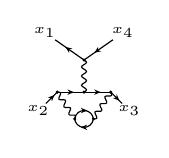
\begin{tikzpicture}[x=0.340cm, y=0.340cm, line width=0.420pt, baseline={([yshift=-0.6ex]0,0)}]
  \draw (0.000,0.133) -- (1.000,0.133);
  \fill (0.619,0.133) -- (0.381,0.235) -- (0.458,0.133) -- (0.381,0.031) -- cycle;
  \draw (-1.000,0.133) -- (0.000,0.133);
  \fill (-0.381,0.133) -- (-0.619,0.235) -- (-0.542,0.133) -- (-0.619,0.031) -- cycle;
  \draw (0.350,-0.867) arc[start angle=353.974, end angle=186.026, radius=0.352];
  \fill (-0.119,-1.182) -- (0.119,-1.284) -- (0.042,-1.182) -- (0.119,-1.080) -- cycle;
  \draw (-0.350,-0.867) arc[start angle=173.974, end angle=6.026, radius=0.352];
  \fill (0.119,-0.552) -- (-0.119,-0.450) -- (-0.042,-0.552) -- (-0.119,-0.654) -- cycle;
  \draw plot[smooth, tension=0.7] coordinates {(0.000,1.333) (0.065,1.290) (0.093,1.248) (0.065,1.205) (0.000,1.162) (-0.065,1.119) (-0.093,1.076) (-0.065,1.033) (0.000,0.990) (0.065,0.948) (0.093,0.905) (0.065,0.862) (0.000,0.819) (-0.065,0.776) (-0.093,0.733) (-0.065,0.690) (0.000,0.648) (0.065,0.605) (0.093,0.562) (0.065,0.519) (0.000,0.476) (-0.065,0.433) (-0.093,0.390) (-0.065,0.348) (0.000,0.305) (0.065,0.262) (0.093,0.219) (0.065,0.176) (0.000,0.133)};
  \draw plot[smooth, tension=0.7] coordinates {(-1.000,0.133) (-0.922,0.133) (-0.876,0.112) (-0.876,0.062) (-0.907,-0.010) (-0.938,-0.081) (-0.938,-0.131) (-0.892,-0.152) (-0.814,-0.152) (-0.737,-0.153) (-0.691,-0.174) (-0.690,-0.224) (-0.721,-0.295) (-0.753,-0.366) (-0.752,-0.417) (-0.706,-0.438) (-0.629,-0.438) (-0.551,-0.438) (-0.505,-0.459) (-0.504,-0.510) (-0.536,-0.581) (-0.567,-0.652) (-0.566,-0.703) (-0.521,-0.724) (-0.443,-0.724) (-0.365,-0.724) (-0.319,-0.745) (-0.319,-0.795) (-0.350,-0.867)};
  \draw plot[smooth, tension=0.7] coordinates {(1.000,0.133) (1.031,0.062) (1.031,0.012) (0.985,-0.009) (0.907,-0.010) (0.829,-0.010) (0.784,-0.031) (0.783,-0.081) (0.814,-0.152) (0.846,-0.224) (0.845,-0.274) (0.799,-0.295) (0.721,-0.295) (0.644,-0.295) (0.598,-0.317) (0.597,-0.367) (0.629,-0.438) (0.660,-0.509) (0.659,-0.560) (0.613,-0.581) (0.536,-0.581) (0.458,-0.581) (0.412,-0.602) (0.412,-0.653) (0.443,-0.724) (0.474,-0.795) (0.474,-0.845) (0.428,-0.866) (0.350,-0.867)};
  \draw (0.000,1.333) -- (-1.081,2.090);
  \fill (-0.693,1.818) -- (-0.555,1.598) -- (-0.560,1.726) -- (-0.438,1.765) -- cycle;
  \draw (-1.000,0.133) -- (-1.424,-0.291);
  \fill (-1.106,0.027) -- (-1.347,-0.070) -- (-1.220,-0.087) -- (-1.203,-0.214) -- cycle;
  \draw (1.000,0.133) -- (1.424,-0.291);
  \fill (1.318,-0.184) -- (1.221,0.057) -- (1.204,-0.070) -- (1.077,-0.088) -- cycle;
  \draw (0.000,1.333) -- (1.081,2.090);
  \fill (0.389,1.606) -- (0.643,1.659) -- (0.521,1.698) -- (0.526,1.826) -- cycle;
  \fill (0.000,1.333) circle (0.064);
  \fill (-1.000,0.133) circle (0.064);
  \fill (1.000,0.133) circle (0.064);
  \fill (0.000,0.133) circle (0.064);
  \fill (-0.350,-0.867) circle (0.064);
  \fill (0.350,-0.867) circle (0.064);
  \node[font=\tiny, inner sep=0pt, anchor=325] at (-1.155,2.142) {$x_{1}$};
  \node[font=\tiny, inner sep=0pt, anchor=45] at (-1.488,-0.355) {$x_{2}$};
  \node[font=\tiny, inner sep=0pt, anchor=135] at (1.488,-0.355) {$x_{3}$};
  \node[font=\tiny, inner sep=0pt, anchor=215] at (1.155,2.142) {$x_{4}$};
\end{tikzpicture}}
\diagramgap
\mbox{$\displaystyle +\,$\,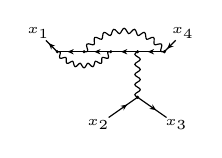
\begin{tikzpicture}[x=0.340cm, y=0.340cm, line width=0.420pt, baseline={([yshift=-0.6ex]0,0)}]
  \draw (-1.167,0.283) -- (-2.167,0.283);
  \fill (-1.786,0.283) -- (-1.547,0.181) -- (-1.625,0.283) -- (-1.547,0.385) -- cycle;
  \draw (1.833,0.283) -- (0.833,0.283);
  \fill (1.214,0.283) -- (1.453,0.181) -- (1.375,0.283) -- (1.453,0.385) -- cycle;
  \draw (-0.167,0.283) -- (-1.167,0.283);
  \fill (-0.786,0.283) -- (-0.547,0.181) -- (-0.625,0.283) -- (-0.547,0.385) -- cycle;
  \draw (0.833,0.283) -- (-0.167,0.283);
  \fill (0.214,0.283) -- (0.453,0.181) -- (0.375,0.283) -- (0.453,0.385) -- cycle;
  \draw plot[smooth, tension=0.7] coordinates {(-2.167,0.283) (-2.098,0.286) (-2.056,0.272) (-2.051,0.228) (-2.069,0.162) (-2.083,0.093) (-2.071,0.047) (-2.025,0.036) (-1.957,0.053) (-1.891,0.073) (-1.847,0.070) (-1.831,0.029) (-1.831,-0.040) (-1.828,-0.110) (-1.804,-0.151) (-1.757,-0.150) (-1.695,-0.116) (-1.637,-0.080) (-1.593,-0.073) (-1.568,-0.108) (-1.551,-0.175) (-1.530,-0.242) (-1.496,-0.276) (-1.450,-0.262) (-1.400,-0.214) (-1.352,-0.164) (-1.312,-0.146) (-1.278,-0.174) (-1.245,-0.234) (-1.208,-0.293) (-1.167,-0.318) (-1.126,-0.293) (-1.089,-0.234) (-1.055,-0.174) (-1.021,-0.146) (-0.981,-0.164) (-0.934,-0.214) (-0.883,-0.262) (-0.837,-0.276) (-0.804,-0.242) (-0.783,-0.175) (-0.766,-0.108) (-0.740,-0.073) (-0.697,-0.080) (-0.638,-0.116) (-0.577,-0.150) (-0.529,-0.151) (-0.505,-0.110) (-0.502,-0.040) (-0.502,0.029) (-0.486,0.070) (-0.443,0.073) (-0.377,0.053) (-0.309,0.036) (-0.262,0.047) (-0.250,0.093) (-0.264,0.162) (-0.282,0.228) (-0.277,0.272) (-0.236,0.286) (-0.167,0.283)};
  \draw plot[smooth, tension=0.7] coordinates {(0.833,-1.417) (0.761,-1.369) (0.731,-1.322) (0.761,-1.275) (0.833,-1.228) (0.905,-1.181) (0.935,-1.133) (0.905,-1.086) (0.833,-1.039) (0.761,-0.992) (0.731,-0.944) (0.761,-0.897) (0.833,-0.850) (0.905,-0.803) (0.935,-0.756) (0.905,-0.708) (0.833,-0.661) (0.761,-0.614) (0.731,-0.567) (0.761,-0.519) (0.833,-0.472) (0.905,-0.425) (0.935,-0.378) (0.905,-0.331) (0.833,-0.283) (0.761,-0.236) (0.731,-0.189) (0.761,-0.142) (0.833,-0.094) (0.905,-0.047) (0.935,0.000) (0.905,0.047) (0.833,0.094) (0.761,0.142) (0.731,0.189) (0.761,0.236) (0.833,0.283)};
  \draw plot[smooth, tension=0.7] coordinates {(1.833,0.283) (1.752,0.280) (1.702,0.299) (1.697,0.351) (1.720,0.429) (1.739,0.510) (1.727,0.564) (1.673,0.579) (1.592,0.563) (1.512,0.543) (1.461,0.551) (1.445,0.601) (1.451,0.683) (1.454,0.765) (1.431,0.816) (1.376,0.820) (1.299,0.788) (1.225,0.753) (1.173,0.751) (1.147,0.796) (1.137,0.877) (1.124,0.959) (1.091,1.004) (1.036,0.997) (0.967,0.950) (0.902,0.901) (0.851,0.888) (0.817,0.928) (0.791,1.005) (0.761,1.083) (0.720,1.120) (0.667,1.102) (0.610,1.042) (0.555,0.981) (0.508,0.958) (0.467,0.990) (0.426,1.061) (0.381,1.131) (0.333,1.160) (0.285,1.131) (0.241,1.061) (0.200,0.990) (0.158,0.958) (0.111,0.981) (0.057,1.042) (-0.001,1.102) (-0.053,1.120) (-0.095,1.083) (-0.124,1.005) (-0.150,0.928) (-0.184,0.888) (-0.235,0.901) (-0.301,0.950) (-0.369,0.997) (-0.424,1.004) (-0.457,0.959) (-0.471,0.877) (-0.481,0.796) (-0.506,0.751) (-0.559,0.753) (-0.633,0.788) (-0.709,0.820) (-0.765,0.816) (-0.788,0.765) (-0.785,0.683) (-0.778,0.601) (-0.794,0.551) (-0.846,0.543) (-0.925,0.563) (-1.006,0.579) (-1.060,0.564) (-1.073,0.510) (-1.053,0.429) (-1.030,0.351) (-1.036,0.299) (-1.085,0.280) (-1.167,0.283)};
  \draw (-2.167,0.283) -- (-2.591,0.708);
  \fill (-2.484,0.601) -- (-2.388,0.360) -- (-2.370,0.487) -- (-2.243,0.504) -- cycle;
  \draw (0.833,-1.417) -- (-0.248,-2.174);
  \fill (0.445,-1.689) -- (0.190,-1.742) -- (0.313,-1.781) -- (0.307,-1.909) -- cycle;
  \draw (0.833,-1.417) -- (1.915,-2.174);
  \fill (1.526,-1.902) -- (1.389,-1.681) -- (1.394,-1.809) -- (1.272,-1.848) -- cycle;
  \draw (1.833,0.283) -- (2.258,0.708);
  \fill (1.940,0.390) -- (2.181,0.487) -- (2.054,0.504) -- (2.037,0.631) -- cycle;
  \fill (-2.167,0.283) circle (0.064);
  \fill (0.833,-1.417) circle (0.064);
  \fill (1.833,0.283) circle (0.064);
  \fill (0.833,0.283) circle (0.064);
  \fill (-1.167,0.283) circle (0.064);
  \fill (-0.167,0.283) circle (0.064);
  \node[font=\tiny, inner sep=0pt, anchor=315] at (-2.655,0.771) {$x_{1}$};
  \node[font=\tiny, inner sep=0pt, anchor=35] at (-0.322,-2.225) {$x_{2}$};
  \node[font=\tiny, inner sep=0pt, anchor=145] at (1.988,-2.225) {$x_{3}$};
  \node[font=\tiny, inner sep=0pt, anchor=225] at (2.321,0.771) {$x_{4}$};
\end{tikzpicture}}
\diagramgap
\mbox{$\displaystyle +\,$\,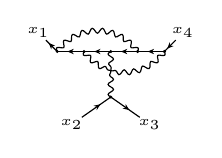
\begin{tikzpicture}[x=0.340cm, y=0.340cm, line width=0.420pt, baseline={([yshift=-0.6ex]0,0)}]
  \draw (-1.000,0.283) -- (-2.000,0.283);
  \fill (-1.619,0.283) -- (-1.381,0.181) -- (-1.458,0.283) -- (-1.381,0.385) -- cycle;
  \draw (2.000,0.283) -- (1.000,0.283);
  \fill (1.381,0.283) -- (1.619,0.181) -- (1.542,0.283) -- (1.619,0.385) -- cycle;
  \draw (0.000,0.283) -- (-1.000,0.283);
  \fill (-0.619,0.283) -- (-0.381,0.181) -- (-0.458,0.283) -- (-0.381,0.385) -- cycle;
  \draw (1.000,0.283) -- (0.000,0.283);
  \fill (0.381,0.283) -- (0.619,0.181) -- (0.542,0.283) -- (0.619,0.385) -- cycle;
  \draw plot[smooth, tension=0.7] coordinates {(-2.000,0.283) (-2.028,0.361) (-2.021,0.417) (-1.969,0.437) (-1.886,0.429) (-1.805,0.418) (-1.755,0.431) (-1.744,0.482) (-1.759,0.563) (-1.770,0.645) (-1.752,0.698) (-1.697,0.707) (-1.618,0.683) (-1.541,0.656) (-1.488,0.658) (-1.468,0.706) (-1.466,0.788) (-1.461,0.871) (-1.433,0.919) (-1.377,0.917) (-1.304,0.877) (-1.234,0.835) (-1.182,0.828) (-1.152,0.870) (-1.134,0.950) (-1.112,1.030) (-1.075,1.072) (-1.021,1.059) (-0.958,1.005) (-0.897,0.950) (-0.848,0.932) (-0.810,0.968) (-0.776,1.042) (-0.739,1.116) (-0.694,1.150) (-0.644,1.126) (-0.592,1.061) (-0.545,0.995) (-0.500,0.967) (-0.455,0.995) (-0.408,1.061) (-0.356,1.126) (-0.306,1.150) (-0.261,1.116) (-0.224,1.042) (-0.190,0.968) (-0.152,0.932) (-0.103,0.950) (-0.042,1.005) (0.021,1.059) (0.075,1.072) (0.112,1.030) (0.134,0.950) (0.152,0.870) (0.182,0.828) (0.234,0.835) (0.304,0.877) (0.377,0.917) (0.433,0.919) (0.461,0.871) (0.466,0.788) (0.468,0.706) (0.488,0.658) (0.541,0.656) (0.618,0.683) (0.697,0.707) (0.752,0.698) (0.770,0.645) (0.759,0.563) (0.744,0.482) (0.755,0.431) (0.805,0.418) (0.886,0.429) (0.969,0.437) (1.021,0.417) (1.028,0.361) (1.000,0.283)};
  \draw plot[smooth, tension=0.7] coordinates {(0.000,-1.417) (-0.072,-1.369) (-0.102,-1.322) (-0.072,-1.275) (0.000,-1.228) (0.072,-1.181) (0.102,-1.133) (0.072,-1.086) (0.000,-1.039) (-0.072,-0.992) (-0.102,-0.944) (-0.072,-0.897) (0.000,-0.850) (0.072,-0.803) (0.102,-0.756) (0.067,-0.708) (0.000,-0.661) (-0.042,-0.614) (-0.038,-0.567) (-0.013,-0.519) (0.000,-0.472) (0.000,-0.425) (0.006,-0.378) (0.014,-0.331) (0.000,-0.283) (-0.042,-0.236) (-0.080,-0.189) (-0.067,-0.142) (0.000,-0.094) (0.072,-0.047) (0.102,0.000) (0.072,0.047) (0.000,0.094) (-0.072,0.142) (-0.102,0.189) (-0.072,0.236) (0.000,0.283)};
  \draw plot[smooth, tension=0.7] coordinates {(2.000,0.283) (2.028,0.205) (2.021,0.150) (1.969,0.130) (1.886,0.138) (1.805,0.149) (1.755,0.136) (1.744,0.084) (1.759,0.004) (1.770,-0.078) (1.752,-0.131) (1.697,-0.140) (1.618,-0.116) (1.541,-0.089) (1.488,-0.092) (1.468,-0.140) (1.466,-0.221) (1.461,-0.304) (1.433,-0.352) (1.377,-0.350) (1.304,-0.311) (1.234,-0.269) (1.182,-0.261) (1.152,-0.304) (1.134,-0.383) (1.112,-0.463) (1.075,-0.505) (1.021,-0.492) (0.958,-0.439) (0.897,-0.383) (0.848,-0.365) (0.810,-0.401) (0.776,-0.476) (0.739,-0.550) (0.694,-0.583) (0.644,-0.559) (0.592,-0.494) (0.545,-0.428) (0.500,-0.400) (0.455,-0.428) (0.408,-0.494) (0.356,-0.559) (0.306,-0.583) (0.262,-0.544) (0.224,-0.476) (0.185,-0.430) (0.140,-0.425) (0.090,-0.438) (0.042,-0.439) (-0.002,-0.427) (-0.048,-0.419) (-0.095,-0.412) (-0.134,-0.383) (-0.162,-0.330) (-0.190,-0.280) (-0.236,-0.273) (-0.304,-0.311) (-0.377,-0.350) (-0.433,-0.352) (-0.461,-0.304) (-0.466,-0.221) (-0.468,-0.140) (-0.488,-0.092) (-0.541,-0.089) (-0.618,-0.116) (-0.697,-0.140) (-0.752,-0.131) (-0.770,-0.078) (-0.759,0.004) (-0.744,0.084) (-0.755,0.136) (-0.805,0.149) (-0.886,0.138) (-0.969,0.130) (-1.021,0.150) (-1.028,0.205) (-1.000,0.283)};
  \draw (-2.000,0.283) -- (-2.424,0.708);
  \fill (-2.318,0.601) -- (-2.221,0.360) -- (-2.204,0.487) -- (-2.077,0.504) -- cycle;
  \draw (0.000,-1.417) -- (-1.081,-2.174);
  \fill (-0.389,-1.689) -- (-0.643,-1.742) -- (-0.521,-1.781) -- (-0.526,-1.909) -- cycle;
  \draw (0.000,-1.417) -- (1.081,-2.174);
  \fill (0.693,-1.902) -- (0.555,-1.681) -- (0.560,-1.809) -- (0.438,-1.848) -- cycle;
  \draw (2.000,0.283) -- (2.424,0.708);
  \fill (2.106,0.390) -- (2.347,0.487) -- (2.220,0.504) -- (2.203,0.631) -- cycle;
  \fill (-2.000,0.283) circle (0.064);
  \fill (0.000,-1.417) circle (0.064);
  \fill (2.000,0.283) circle (0.064);
  \fill (1.000,0.283) circle (0.064);
  \fill (-1.000,0.283) circle (0.064);
  \fill (0.000,0.283) circle (0.064);
  \node[font=\tiny, inner sep=0pt, anchor=315] at (-2.488,0.771) {$x_{1}$};
  \node[font=\tiny, inner sep=0pt, anchor=35] at (-1.155,-2.225) {$x_{2}$};
  \node[font=\tiny, inner sep=0pt, anchor=145] at (1.155,-2.225) {$x_{3}$};
  \node[font=\tiny, inner sep=0pt, anchor=225] at (2.488,0.771) {$x_{4}$};
\end{tikzpicture}}
\diagramgap
\mbox{$\displaystyle -\,$\,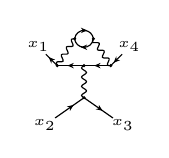
\begin{tikzpicture}[x=0.340cm, y=0.340cm, line width=0.420pt, baseline={([yshift=-0.6ex]0,0)}]
  \draw (0.000,-0.133) -- (-1.000,-0.133);
  \fill (-0.619,-0.133) -- (-0.381,-0.235) -- (-0.458,-0.133) -- (-0.381,-0.031) -- cycle;
  \draw (1.000,-0.133) -- (0.000,-0.133);
  \fill (0.381,-0.133) -- (0.619,-0.235) -- (0.542,-0.133) -- (0.619,-0.031) -- cycle;
  \draw (0.350,0.867) arc[start angle=353.974, end angle=186.026, radius=0.352];
  \fill (-0.119,0.552) -- (0.119,0.450) -- (0.042,0.552) -- (0.119,0.654) -- cycle;
  \draw (-0.350,0.867) arc[start angle=173.974, end angle=6.026, radius=0.352];
  \fill (0.119,1.182) -- (-0.119,1.284) -- (-0.042,1.182) -- (-0.119,1.080) -- cycle;
  \draw plot[smooth, tension=0.7] coordinates {(-1.000,-0.133) (-1.031,-0.062) (-1.031,-0.012) (-0.985,0.009) (-0.907,0.010) (-0.829,0.010) (-0.784,0.031) (-0.783,0.081) (-0.814,0.152) (-0.846,0.224) (-0.845,0.274) (-0.799,0.295) (-0.721,0.295) (-0.644,0.295) (-0.598,0.317) (-0.597,0.367) (-0.629,0.438) (-0.660,0.509) (-0.659,0.560) (-0.613,0.581) (-0.536,0.581) (-0.458,0.581) (-0.412,0.602) (-0.412,0.653) (-0.443,0.724) (-0.474,0.795) (-0.474,0.845) (-0.428,0.866) (-0.350,0.867)};
  \draw plot[smooth, tension=0.7] coordinates {(0.000,-1.333) (-0.065,-1.290) (-0.093,-1.248) (-0.065,-1.205) (0.000,-1.162) (0.065,-1.119) (0.093,-1.076) (0.065,-1.033) (0.000,-0.990) (-0.065,-0.948) (-0.093,-0.905) (-0.065,-0.862) (0.000,-0.819) (0.065,-0.776) (0.093,-0.733) (0.065,-0.690) (0.000,-0.648) (-0.065,-0.605) (-0.093,-0.562) (-0.065,-0.519) (0.000,-0.476) (0.065,-0.433) (0.093,-0.390) (0.065,-0.348) (0.000,-0.305) (-0.065,-0.262) (-0.093,-0.219) (-0.065,-0.176) (0.000,-0.133)};
  \draw plot[smooth, tension=0.7] coordinates {(1.000,-0.133) (0.922,-0.133) (0.876,-0.112) (0.876,-0.062) (0.907,0.010) (0.938,0.081) (0.938,0.131) (0.892,0.152) (0.814,0.152) (0.737,0.153) (0.691,0.174) (0.690,0.224) (0.721,0.295) (0.753,0.366) (0.752,0.417) (0.706,0.438) (0.629,0.438) (0.551,0.438) (0.505,0.459) (0.504,0.510) (0.536,0.581) (0.567,0.652) (0.566,0.703) (0.521,0.724) (0.443,0.724) (0.365,0.724) (0.319,0.745) (0.319,0.795) (0.350,0.867)};
  \draw (-1.000,-0.133) -- (-1.424,0.291);
  \fill (-1.318,0.184) -- (-1.221,-0.057) -- (-1.204,0.070) -- (-1.077,0.088) -- cycle;
  \draw (0.000,-1.333) -- (-1.081,-2.090);
  \fill (-0.389,-1.606) -- (-0.643,-1.659) -- (-0.521,-1.698) -- (-0.526,-1.826) -- cycle;
  \draw (0.000,-1.333) -- (1.081,-2.090);
  \fill (0.693,-1.818) -- (0.555,-1.598) -- (0.560,-1.726) -- (0.438,-1.765) -- cycle;
  \draw (1.000,-0.133) -- (1.424,0.291);
  \fill (1.106,-0.027) -- (1.347,0.070) -- (1.220,0.087) -- (1.203,0.214) -- cycle;
  \fill (-1.000,-0.133) circle (0.064);
  \fill (0.000,-1.333) circle (0.064);
  \fill (1.000,-0.133) circle (0.064);
  \fill (0.000,-0.133) circle (0.064);
  \fill (-0.350,0.867) circle (0.064);
  \fill (0.350,0.867) circle (0.064);
  \node[font=\tiny, inner sep=0pt, anchor=315] at (-1.488,0.355) {$x_{1}$};
  \node[font=\tiny, inner sep=0pt, anchor=35] at (-1.155,-2.142) {$x_{2}$};
  \node[font=\tiny, inner sep=0pt, anchor=145] at (1.155,-2.142) {$x_{3}$};
  \node[font=\tiny, inner sep=0pt, anchor=225] at (1.488,0.355) {$x_{4}$};
\end{tikzpicture}}
\diagramgap
\mbox{$\displaystyle +\,$\,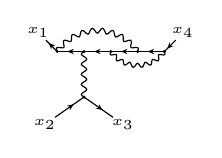
\begin{tikzpicture}[x=0.340cm, y=0.340cm, line width=0.420pt, baseline={([yshift=-0.6ex]0,0)}]
  \draw (-0.833,0.283) -- (-1.833,0.283);
  \fill (-1.453,0.283) -- (-1.214,0.181) -- (-1.292,0.283) -- (-1.214,0.385) -- cycle;
  \draw (2.167,0.283) -- (1.167,0.283);
  \fill (1.547,0.283) -- (1.786,0.181) -- (1.708,0.283) -- (1.786,0.385) -- cycle;
  \draw (0.167,0.283) -- (-0.833,0.283);
  \fill (-0.453,0.283) -- (-0.214,0.181) -- (-0.292,0.283) -- (-0.214,0.385) -- cycle;
  \draw (1.167,0.283) -- (0.167,0.283);
  \fill (0.547,0.283) -- (0.786,0.181) -- (0.708,0.283) -- (0.786,0.385) -- cycle;
  \draw plot[smooth, tension=0.7] coordinates {(-1.833,0.283) (-1.861,0.361) (-1.854,0.417) (-1.802,0.437) (-1.720,0.429) (-1.639,0.418) (-1.588,0.431) (-1.577,0.482) (-1.592,0.563) (-1.603,0.645) (-1.585,0.698) (-1.530,0.707) (-1.451,0.683) (-1.374,0.656) (-1.322,0.658) (-1.301,0.706) (-1.299,0.788) (-1.294,0.871) (-1.266,0.919) (-1.210,0.917) (-1.137,0.877) (-1.067,0.835) (-1.015,0.828) (-0.985,0.870) (-0.967,0.950) (-0.946,1.030) (-0.908,1.072) (-0.854,1.059) (-0.791,1.005) (-0.731,0.950) (-0.681,0.932) (-0.643,0.968) (-0.610,1.042) (-0.572,1.116) (-0.528,1.150) (-0.477,1.126) (-0.426,1.061) (-0.378,0.995) (-0.333,0.967) (-0.289,0.995) (-0.241,1.061) (-0.190,1.126) (-0.139,1.150) (-0.094,1.116) (-0.057,1.042) (-0.023,0.968) (0.015,0.932) (0.064,0.950) (0.124,1.005) (0.187,1.059) (0.242,1.072) (0.279,1.030) (0.301,0.950) (0.319,0.870) (0.349,0.828) (0.401,0.835) (0.471,0.877) (0.543,0.917) (0.599,0.919) (0.627,0.871) (0.633,0.788) (0.634,0.706) (0.655,0.658) (0.707,0.656) (0.785,0.683) (0.864,0.707) (0.919,0.698) (0.937,0.645) (0.925,0.563) (0.910,0.482) (0.921,0.431) (0.972,0.418) (1.053,0.429) (1.135,0.437) (1.188,0.417) (1.194,0.361) (1.167,0.283)};
  \draw plot[smooth, tension=0.7] coordinates {(-0.833,-1.417) (-0.905,-1.369) (-0.935,-1.322) (-0.905,-1.275) (-0.833,-1.228) (-0.761,-1.181) (-0.731,-1.133) (-0.761,-1.086) (-0.833,-1.039) (-0.905,-0.992) (-0.935,-0.944) (-0.905,-0.897) (-0.833,-0.850) (-0.761,-0.803) (-0.731,-0.756) (-0.761,-0.708) (-0.833,-0.661) (-0.905,-0.614) (-0.935,-0.567) (-0.905,-0.519) (-0.833,-0.472) (-0.761,-0.425) (-0.731,-0.378) (-0.761,-0.331) (-0.833,-0.283) (-0.905,-0.236) (-0.935,-0.189) (-0.905,-0.142) (-0.833,-0.094) (-0.761,-0.047) (-0.731,0.000) (-0.761,0.047) (-0.833,0.094) (-0.905,0.142) (-0.935,0.189) (-0.905,0.236) (-0.833,0.283)};
  \draw plot[smooth, tension=0.7] coordinates {(2.167,0.283) (2.190,0.217) (2.183,0.170) (2.139,0.153) (2.069,0.162) (2.001,0.173) (1.958,0.164) (1.948,0.122) (1.957,0.053) (1.962,-0.017) (1.944,-0.061) (1.897,-0.065) (1.831,-0.040) (1.769,-0.012) (1.725,-0.010) (1.704,-0.048) (1.695,-0.116) (1.683,-0.185) (1.654,-0.223) (1.607,-0.216) (1.551,-0.175) (1.497,-0.131) (1.455,-0.118) (1.425,-0.150) (1.400,-0.214) (1.370,-0.278) (1.333,-0.307) (1.289,-0.288) (1.245,-0.234) (1.204,-0.179) (1.167,-0.155) (1.129,-0.179) (1.089,-0.234) (1.044,-0.288) (1.001,-0.307) (0.963,-0.278) (0.934,-0.214) (0.908,-0.150) (0.878,-0.118) (0.836,-0.131) (0.783,-0.175) (0.726,-0.216) (0.679,-0.223) (0.650,-0.185) (0.638,-0.116) (0.630,-0.048) (0.609,-0.010) (0.565,-0.012) (0.502,-0.040) (0.437,-0.065) (0.389,-0.061) (0.371,-0.017) (0.377,0.053) (0.386,0.122) (0.375,0.164) (0.332,0.173) (0.264,0.162) (0.195,0.153) (0.150,0.170) (0.144,0.217) (0.167,0.283)};
  \draw (-1.833,0.283) -- (-2.258,0.708);
  \fill (-2.151,0.601) -- (-2.054,0.360) -- (-2.037,0.487) -- (-1.910,0.504) -- cycle;
  \draw (-0.833,-1.417) -- (-1.915,-2.174);
  \fill (-1.222,-1.689) -- (-1.476,-1.742) -- (-1.354,-1.781) -- (-1.359,-1.909) -- cycle;
  \draw (-0.833,-1.417) -- (0.248,-2.174);
  \fill (-0.141,-1.902) -- (-0.278,-1.681) -- (-0.273,-1.809) -- (-0.395,-1.848) -- cycle;
  \draw (2.167,0.283) -- (2.591,0.708);
  \fill (2.273,0.390) -- (2.514,0.487) -- (2.387,0.504) -- (2.370,0.631) -- cycle;
  \fill (-1.833,0.283) circle (0.064);
  \fill (-0.833,-1.417) circle (0.064);
  \fill (2.167,0.283) circle (0.064);
  \fill (1.167,0.283) circle (0.064);
  \fill (-0.833,0.283) circle (0.064);
  \fill (0.167,0.283) circle (0.064);
  \node[font=\tiny, inner sep=0pt, anchor=315] at (-2.321,0.771) {$x_{1}$};
  \node[font=\tiny, inner sep=0pt, anchor=35] at (-1.988,-2.225) {$x_{2}$};
  \node[font=\tiny, inner sep=0pt, anchor=145] at (0.322,-2.225) {$x_{3}$};
  \node[font=\tiny, inner sep=0pt, anchor=225] at (2.655,0.771) {$x_{4}$};
\end{tikzpicture}}
\diagramgap
\mbox{$\displaystyle -\,$\,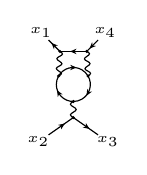
\begin{tikzpicture}[x=0.340cm, y=0.340cm, line width=0.420pt, baseline={([yshift=-0.6ex]0,0)}]
  \draw (0.500,1.029) -- (-0.500,1.029);
  \fill (-0.119,1.029) -- (0.119,0.927) -- (0.042,1.029) -- (0.119,1.131) -- cycle;
  \draw (0.000,-0.841) arc[start angle=270.000, end angle=150.000, radius=0.635];
  \fill (-0.610,-0.420) -- (-0.579,-0.678) -- (-0.529,-0.560) -- (-0.402,-0.576) -- cycle;
  \draw (0.550,0.112) arc[start angle=30.000, end angle=-90.000, radius=0.635];
  \fill (0.490,-0.627) -- (0.698,-0.471) -- (0.571,-0.487) -- (0.521,-0.369) -- cycle;
  \draw (-0.550,0.112) arc[start angle=150.000, end angle=30.000, radius=0.635];
  \fill (0.119,0.429) -- (-0.119,0.531) -- (-0.042,0.429) -- (-0.119,0.327) -- cycle;
  \draw plot[smooth, tension=0.7] coordinates {(-0.500,1.029) (-0.432,0.980) (-0.406,0.932) (-0.437,0.888) (-0.510,0.846) (-0.583,0.804) (-0.614,0.759) (-0.588,0.712) (-0.520,0.662) (-0.452,0.613) (-0.426,0.565) (-0.457,0.521) (-0.530,0.479) (-0.603,0.437) (-0.634,0.392) (-0.608,0.345) (-0.540,0.295) (-0.472,0.246) (-0.446,0.198) (-0.477,0.154) (-0.550,0.112)};
  \draw plot[smooth, tension=0.7] coordinates {(0.000,-1.441) (-0.076,-1.391) (-0.108,-1.341) (-0.076,-1.291) (0.000,-1.241) (0.076,-1.191) (0.108,-1.141) (0.076,-1.091) (0.000,-1.041) (-0.076,-0.991) (-0.108,-0.941) (-0.076,-0.891) (0.000,-0.841)};
  \draw plot[smooth, tension=0.7] coordinates {(0.500,1.029) (0.573,0.987) (0.604,0.943) (0.578,0.895) (0.510,0.846) (0.442,0.796) (0.416,0.749) (0.447,0.704) (0.520,0.662) (0.593,0.620) (0.624,0.576) (0.598,0.528) (0.530,0.479) (0.462,0.429) (0.436,0.382) (0.467,0.337) (0.540,0.295) (0.613,0.253) (0.644,0.209) (0.618,0.161) (0.550,0.112)};
  \draw (-0.500,1.029) -- (-0.924,1.454);
  \fill (-0.818,1.347) -- (-0.721,1.106) -- (-0.704,1.233) -- (-0.577,1.250) -- cycle;
  \draw (0.000,-1.441) -- (-0.924,-2.088);
  \fill (-0.318,-1.664) -- (-0.572,-1.717) -- (-0.450,-1.756) -- (-0.455,-1.884) -- cycle;
  \draw (0.000,-1.441) -- (0.924,-2.088);
  \fill (0.606,-1.865) -- (0.469,-1.645) -- (0.474,-1.773) -- (0.352,-1.812) -- cycle;
  \draw (0.500,1.029) -- (0.924,1.454);
  \fill (0.606,1.136) -- (0.847,1.232) -- (0.720,1.250) -- (0.703,1.377) -- cycle;
  \fill (-0.500,1.029) circle (0.064);
  \fill (0.000,-1.441) circle (0.064);
  \fill (0.500,1.029) circle (0.064);
  \fill (-0.550,0.112) circle (0.064);
  \fill (0.000,-0.841) circle (0.064);
  \fill (0.550,0.112) circle (0.064);
  \node[font=\tiny, inner sep=0pt, anchor=315] at (-0.988,1.517) {$x_{1}$};
  \node[font=\tiny, inner sep=0pt, anchor=35] at (-0.998,-2.140) {$x_{2}$};
  \node[font=\tiny, inner sep=0pt, anchor=145] at (0.998,-2.140) {$x_{3}$};
  \node[font=\tiny, inner sep=0pt, anchor=225] at (0.988,1.517) {$x_{4}$};
\end{tikzpicture}}
\diagramgap
\mbox{$\displaystyle -\,$\,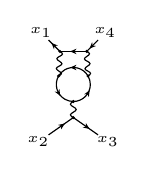
\begin{tikzpicture}[x=0.340cm, y=0.340cm, line width=0.420pt, baseline={([yshift=-0.6ex]0,0)}]
  \draw (0.500,1.029) -- (-0.500,1.029);
  \fill (-0.119,1.029) -- (0.119,0.927) -- (0.042,1.029) -- (0.119,1.131) -- cycle;
  \draw (0.550,0.112) arc[start angle=30.000, end angle=150.000, radius=0.635];
  \fill (-0.119,0.429) -- (0.119,0.327) -- (0.042,0.429) -- (0.119,0.531) -- cycle;
  \draw (-0.550,0.112) arc[start angle=150.000, end angle=270.000, radius=0.635];
  \fill (-0.490,-0.627) -- (-0.521,-0.369) -- (-0.571,-0.487) -- (-0.698,-0.471) -- cycle;
  \draw (0.000,-0.841) arc[start angle=270.000, end angle=390.000, radius=0.635];
  \fill (0.610,-0.420) -- (0.402,-0.576) -- (0.529,-0.560) -- (0.579,-0.678) -- cycle;
  \draw plot[smooth, tension=0.7] coordinates {(-0.500,1.029) (-0.432,0.980) (-0.406,0.932) (-0.437,0.888) (-0.510,0.846) (-0.583,0.804) (-0.614,0.759) (-0.588,0.712) (-0.520,0.662) (-0.452,0.613) (-0.426,0.565) (-0.457,0.521) (-0.530,0.479) (-0.603,0.437) (-0.634,0.392) (-0.608,0.345) (-0.540,0.295) (-0.472,0.246) (-0.446,0.198) (-0.477,0.154) (-0.550,0.112)};
  \draw plot[smooth, tension=0.7] coordinates {(0.000,-1.441) (-0.076,-1.391) (-0.108,-1.341) (-0.076,-1.291) (0.000,-1.241) (0.076,-1.191) (0.108,-1.141) (0.076,-1.091) (0.000,-1.041) (-0.076,-0.991) (-0.108,-0.941) (-0.076,-0.891) (0.000,-0.841)};
  \draw plot[smooth, tension=0.7] coordinates {(0.500,1.029) (0.573,0.987) (0.604,0.943) (0.578,0.895) (0.510,0.846) (0.442,0.796) (0.416,0.749) (0.447,0.704) (0.520,0.662) (0.593,0.620) (0.624,0.576) (0.598,0.528) (0.530,0.479) (0.462,0.429) (0.436,0.382) (0.467,0.337) (0.540,0.295) (0.613,0.253) (0.644,0.209) (0.618,0.161) (0.550,0.112)};
  \draw (-0.500,1.029) -- (-0.924,1.454);
  \fill (-0.818,1.347) -- (-0.721,1.106) -- (-0.704,1.233) -- (-0.577,1.250) -- cycle;
  \draw (0.000,-1.441) -- (-0.924,-2.088);
  \fill (-0.318,-1.664) -- (-0.572,-1.717) -- (-0.450,-1.756) -- (-0.455,-1.884) -- cycle;
  \draw (0.000,-1.441) -- (0.924,-2.088);
  \fill (0.606,-1.865) -- (0.469,-1.645) -- (0.474,-1.773) -- (0.352,-1.812) -- cycle;
  \draw (0.500,1.029) -- (0.924,1.454);
  \fill (0.606,1.136) -- (0.847,1.232) -- (0.720,1.250) -- (0.703,1.377) -- cycle;
  \fill (-0.500,1.029) circle (0.064);
  \fill (0.000,-1.441) circle (0.064);
  \fill (0.500,1.029) circle (0.064);
  \fill (-0.550,0.112) circle (0.064);
  \fill (0.000,-0.841) circle (0.064);
  \fill (0.550,0.112) circle (0.064);
  \node[font=\tiny, inner sep=0pt, anchor=315] at (-0.988,1.517) {$x_{1}$};
  \node[font=\tiny, inner sep=0pt, anchor=35] at (-0.998,-2.140) {$x_{2}$};
  \node[font=\tiny, inner sep=0pt, anchor=145] at (0.998,-2.140) {$x_{3}$};
  \node[font=\tiny, inner sep=0pt, anchor=225] at (0.988,1.517) {$x_{4}$};
\end{tikzpicture}}
\diagramgap
\mbox{$\displaystyle +\,$\,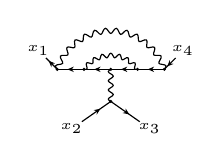
\begin{tikzpicture}[x=0.340cm, y=0.340cm, line width=0.420pt, baseline={([yshift=-0.6ex]0,0)}]
  \draw (-1.000,0.200) -- (-2.000,0.200);
  \fill (-1.619,0.200) -- (-1.381,0.098) -- (-1.458,0.200) -- (-1.381,0.302) -- cycle;
  \draw (2.000,0.200) -- (1.000,0.200);
  \fill (1.381,0.200) -- (1.619,0.098) -- (1.542,0.200) -- (1.619,0.302) -- cycle;
  \draw (0.000,0.200) -- (-1.000,0.200);
  \fill (-0.619,0.200) -- (-0.381,0.098) -- (-0.458,0.200) -- (-0.381,0.302) -- cycle;
  \draw (1.000,0.200) -- (0.000,0.200);
  \fill (0.381,0.200) -- (0.619,0.098) -- (0.542,0.200) -- (0.619,0.302) -- cycle;
  \draw plot[smooth, tension=0.7] coordinates {(-2.000,0.200) (-2.051,0.270) (-2.062,0.328) (-2.015,0.364) (-1.930,0.382) (-1.845,0.396) (-1.798,0.425) (-1.803,0.480) (-1.843,0.556) (-1.881,0.635) (-1.880,0.694) (-1.828,0.721) (-1.740,0.722) (-1.654,0.720) (-1.603,0.740) (-1.598,0.795) (-1.623,0.878) (-1.646,0.962) (-1.634,1.019) (-1.578,1.036) (-1.492,1.022) (-1.407,1.004) (-1.353,1.014) (-1.338,1.067) (-1.348,1.153) (-1.355,1.240) (-1.333,1.294) (-1.274,1.301) (-1.192,1.271) (-1.113,1.238) (-1.057,1.238) (-1.033,1.287) (-1.027,1.373) (-1.017,1.460) (-0.986,1.509) (-0.927,1.505) (-0.852,1.460) (-0.780,1.413) (-0.726,1.403) (-0.692,1.447) (-0.671,1.531) (-0.645,1.614) (-0.605,1.657) (-0.548,1.642) (-0.483,1.584) (-0.421,1.524) (-0.369,1.504) (-0.328,1.542) (-0.292,1.620) (-0.251,1.697) (-0.204,1.732) (-0.151,1.706) (-0.097,1.638) (-0.047,1.568) (0.000,1.539) (0.047,1.568) (0.097,1.638) (0.151,1.706) (0.204,1.732) (0.251,1.697) (0.292,1.620) (0.328,1.542) (0.369,1.504) (0.421,1.524) (0.483,1.584) (0.548,1.642) (0.605,1.657) (0.645,1.614) (0.671,1.531) (0.692,1.447) (0.726,1.403) (0.780,1.413) (0.852,1.460) (0.927,1.505) (0.986,1.509) (1.017,1.460) (1.027,1.373) (1.033,1.287) (1.057,1.238) (1.113,1.238) (1.192,1.271) (1.274,1.301) (1.333,1.294) (1.355,1.240) (1.348,1.153) (1.338,1.067) (1.353,1.014) (1.407,1.004) (1.492,1.022) (1.578,1.036) (1.634,1.019) (1.646,0.962) (1.623,0.878) (1.598,0.795) (1.603,0.740) (1.654,0.720) (1.740,0.722) (1.828,0.721) (1.880,0.694) (1.881,0.635) (1.843,0.556) (1.803,0.480) (1.798,0.425) (1.845,0.396) (1.930,0.382) (2.015,0.364) (2.062,0.328) (2.051,0.270) (2.000,0.200)};
  \draw plot[smooth, tension=0.7] coordinates {(0.000,-1.000) (-0.065,-0.957) (-0.093,-0.914) (-0.065,-0.871) (0.000,-0.829) (0.065,-0.786) (0.093,-0.743) (0.065,-0.700) (0.000,-0.657) (-0.065,-0.614) (-0.093,-0.571) (-0.065,-0.529) (0.000,-0.486) (0.065,-0.443) (0.093,-0.400) (0.065,-0.357) (0.000,-0.314) (-0.065,-0.271) (-0.093,-0.229) (-0.065,-0.186) (0.000,-0.143) (0.065,-0.100) (0.093,-0.057) (0.065,-0.014) (0.000,0.029) (-0.065,0.071) (-0.093,0.114) (-0.065,0.157) (0.000,0.200)};
  \draw plot[smooth, tension=0.7] coordinates {(1.000,0.200) (0.931,0.197) (0.890,0.212) (0.885,0.255) (0.902,0.322) (0.917,0.390) (0.904,0.436) (0.858,0.447) (0.790,0.430) (0.724,0.410) (0.680,0.414) (0.664,0.454) (0.665,0.523) (0.661,0.593) (0.638,0.634) (0.590,0.633) (0.529,0.600) (0.470,0.563) (0.427,0.556) (0.401,0.591) (0.384,0.658) (0.363,0.725) (0.330,0.759) (0.284,0.746) (0.233,0.698) (0.185,0.648) (0.145,0.629) (0.111,0.657) (0.078,0.718) (0.041,0.777) (0.000,0.801) (-0.041,0.777) (-0.078,0.718) (-0.111,0.657) (-0.145,0.629) (-0.185,0.648) (-0.233,0.698) (-0.284,0.746) (-0.330,0.759) (-0.363,0.725) (-0.384,0.658) (-0.401,0.591) (-0.427,0.556) (-0.470,0.563) (-0.529,0.600) (-0.590,0.633) (-0.638,0.634) (-0.661,0.593) (-0.665,0.523) (-0.664,0.454) (-0.680,0.414) (-0.724,0.410) (-0.790,0.430) (-0.858,0.447) (-0.904,0.436) (-0.917,0.390) (-0.902,0.322) (-0.885,0.255) (-0.890,0.212) (-0.931,0.197) (-1.000,0.200)};
  \draw (-2.000,0.200) -- (-2.424,0.624);
  \fill (-2.318,0.518) -- (-2.221,0.277) -- (-2.204,0.404) -- (-2.077,0.421) -- cycle;
  \draw (0.000,-1.000) -- (-1.081,-1.757);
  \fill (-0.389,-1.272) -- (-0.643,-1.326) -- (-0.521,-1.365) -- (-0.526,-1.493) -- cycle;
  \draw (0.000,-1.000) -- (1.081,-1.757);
  \fill (0.693,-1.485) -- (0.555,-1.264) -- (0.560,-1.392) -- (0.438,-1.432) -- cycle;
  \draw (2.000,0.200) -- (2.424,0.624);
  \fill (2.106,0.306) -- (2.347,0.403) -- (2.220,0.420) -- (2.203,0.547) -- cycle;
  \fill (-2.000,0.200) circle (0.064);
  \fill (0.000,-1.000) circle (0.064);
  \fill (2.000,0.200) circle (0.064);
  \fill (1.000,0.200) circle (0.064);
  \fill (-1.000,0.200) circle (0.064);
  \fill (0.000,0.200) circle (0.064);
  \node[font=\tiny, inner sep=0pt, anchor=315] at (-2.488,0.688) {$x_{1}$};
  \node[font=\tiny, inner sep=0pt, anchor=35] at (-1.155,-1.809) {$x_{2}$};
  \node[font=\tiny, inner sep=0pt, anchor=145] at (1.155,-1.809) {$x_{3}$};
  \node[font=\tiny, inner sep=0pt, anchor=225] at (2.488,0.688) {$x_{4}$};
\end{tikzpicture}}
\diagramgap
\mbox{$\displaystyle -\,$\,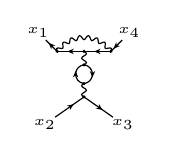
\begin{tikzpicture}[x=0.340cm, y=0.340cm, line width=0.420pt, baseline={([yshift=-0.6ex]0,0)}]
  \draw (0.000,0.567) -- (-1.000,0.567);
  \fill (-0.619,0.567) -- (-0.381,0.465) -- (-0.458,0.567) -- (-0.381,0.669) -- cycle;
  \draw (1.000,0.567) -- (0.000,0.567);
  \fill (0.381,0.567) -- (0.619,0.465) -- (0.542,0.567) -- (0.619,0.669) -- cycle;
  \draw (0.000,0.067) arc[start angle=83.974, end angle=-83.974, radius=0.352];
  \fill (0.315,-0.403) -- (0.417,-0.164) -- (0.315,-0.242) -- (0.213,-0.164) -- cycle;
  \draw (0.000,-0.633) arc[start angle=263.974, end angle=96.026, radius=0.352];
  \fill (-0.315,-0.164) -- (-0.417,-0.403) -- (-0.315,-0.325) -- (-0.213,-0.403) -- cycle;
  \draw plot[smooth, tension=0.7] coordinates {(-1.000,0.567) (-1.023,0.633) (-1.017,0.680) (-0.972,0.697) (-0.902,0.688) (-0.834,0.677) (-0.792,0.686) (-0.781,0.728) (-0.790,0.797) (-0.796,0.867) (-0.777,0.911) (-0.730,0.915) (-0.665,0.890) (-0.602,0.862) (-0.558,0.860) (-0.537,0.898) (-0.529,0.966) (-0.516,1.035) (-0.488,1.073) (-0.441,1.066) (-0.384,1.025) (-0.330,0.981) (-0.288,0.968) (-0.258,1.000) (-0.233,1.064) (-0.204,1.128) (-0.166,1.157) (-0.122,1.138) (-0.078,1.084) (-0.037,1.029) (0.000,1.005) (0.037,1.029) (0.078,1.084) (0.122,1.138) (0.166,1.157) (0.204,1.128) (0.233,1.064) (0.258,1.000) (0.288,0.968) (0.330,0.981) (0.384,1.025) (0.441,1.066) (0.488,1.073) (0.516,1.035) (0.529,0.966) (0.537,0.898) (0.558,0.860) (0.602,0.862) (0.665,0.890) (0.730,0.915) (0.777,0.911) (0.796,0.867) (0.790,0.797) (0.781,0.728) (0.792,0.686) (0.834,0.677) (0.902,0.688) (0.972,0.697) (1.017,0.680) (1.023,0.633) (1.000,0.567)};
  \draw plot[smooth, tension=0.7] coordinates {(0.000,-1.133) (-0.064,-1.092) (-0.090,-1.050) (-0.064,-1.008) (0.000,-0.967) (0.064,-0.925) (0.090,-0.883) (0.064,-0.842) (0.000,-0.800) (-0.064,-0.758) (-0.090,-0.717) (-0.064,-0.675) (0.000,-0.633)};
  \draw plot[smooth, tension=0.7] coordinates {(0.000,0.567) (0.064,0.525) (0.090,0.483) (0.064,0.442) (0.000,0.400) (-0.064,0.358) (-0.090,0.317) (-0.064,0.275) (0.000,0.233) (0.064,0.192) (0.090,0.150) (0.064,0.108) (0.000,0.067)};
  \draw (-1.000,0.567) -- (-1.424,0.991);
  \fill (-1.318,0.884) -- (-1.221,0.643) -- (-1.204,0.770) -- (-1.077,0.788) -- cycle;
  \draw (0.000,-1.133) -- (-1.081,-1.890);
  \fill (-0.389,-1.406) -- (-0.643,-1.459) -- (-0.521,-1.498) -- (-0.526,-1.626) -- cycle;
  \draw (0.000,-1.133) -- (1.081,-1.890);
  \fill (0.693,-1.618) -- (0.555,-1.398) -- (0.560,-1.526) -- (0.438,-1.565) -- cycle;
  \draw (1.000,0.567) -- (1.424,0.991);
  \fill (1.106,0.673) -- (1.347,0.770) -- (1.220,0.787) -- (1.203,0.914) -- cycle;
  \fill (-1.000,0.567) circle (0.064);
  \fill (0.000,-1.133) circle (0.064);
  \fill (1.000,0.567) circle (0.064);
  \fill (0.000,0.567) circle (0.064);
  \fill (0.000,-0.633) circle (0.064);
  \fill (0.000,0.067) circle (0.064);
  \node[font=\tiny, inner sep=0pt, anchor=315] at (-1.488,1.055) {$x_{1}$};
  \node[font=\tiny, inner sep=0pt, anchor=35] at (-1.155,-1.942) {$x_{2}$};
  \node[font=\tiny, inner sep=0pt, anchor=145] at (1.155,-1.942) {$x_{3}$};
  \node[font=\tiny, inner sep=0pt, anchor=225] at (1.488,1.055) {$x_{4}$};
\end{tikzpicture}}
\diagramgap
\mbox{$\displaystyle +\,$\,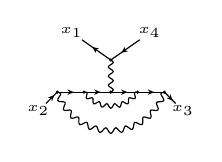
\begin{tikzpicture}[x=0.340cm, y=0.340cm, line width=0.420pt, baseline={([yshift=-0.6ex]0,0)}]
  \draw (1.000,-0.200) -- (2.000,-0.200);
  \fill (1.619,-0.200) -- (1.381,-0.098) -- (1.458,-0.200) -- (1.381,-0.302) -- cycle;
  \draw (-2.000,-0.200) -- (-1.000,-0.200);
  \fill (-1.381,-0.200) -- (-1.619,-0.098) -- (-1.542,-0.200) -- (-1.619,-0.302) -- cycle;
  \draw (0.000,-0.200) -- (1.000,-0.200);
  \fill (0.619,-0.200) -- (0.381,-0.098) -- (0.458,-0.200) -- (0.381,-0.302) -- cycle;
  \draw (-1.000,-0.200) -- (0.000,-0.200);
  \fill (-0.381,-0.200) -- (-0.619,-0.098) -- (-0.542,-0.200) -- (-0.619,-0.302) -- cycle;
  \draw plot[smooth, tension=0.7] coordinates {(0.000,1.000) (0.065,0.957) (0.093,0.914) (0.065,0.871) (0.000,0.829) (-0.065,0.786) (-0.093,0.743) (-0.065,0.700) (0.000,0.657) (0.065,0.614) (0.093,0.571) (0.065,0.529) (0.000,0.486) (-0.065,0.443) (-0.093,0.400) (-0.065,0.357) (0.000,0.314) (0.065,0.271) (0.093,0.229) (0.065,0.186) (0.000,0.143) (-0.065,0.100) (-0.093,0.057) (-0.065,0.014) (0.000,-0.029) (0.065,-0.071) (0.093,-0.114) (0.065,-0.157) (0.000,-0.200)};
  \draw plot[smooth, tension=0.7] coordinates {(-2.000,-0.200) (-1.917,-0.222) (-1.872,-0.255) (-1.883,-0.310) (-1.930,-0.382) (-1.974,-0.457) (-1.979,-0.515) (-1.930,-0.547) (-1.843,-0.556) (-1.757,-0.562) (-1.707,-0.587) (-1.707,-0.642) (-1.740,-0.722) (-1.771,-0.804) (-1.764,-0.862) (-1.710,-0.884) (-1.623,-0.878) (-1.537,-0.868) (-1.484,-0.883) (-1.474,-0.937) (-1.492,-1.022) (-1.506,-1.108) (-1.490,-1.164) (-1.432,-1.176) (-1.348,-1.153) (-1.265,-1.128) (-1.210,-1.133) (-1.190,-1.184) (-1.192,-1.271) (-1.191,-1.358) (-1.164,-1.410) (-1.105,-1.411) (-1.027,-1.373) (-0.950,-1.333) (-0.895,-1.328) (-0.866,-1.375) (-0.852,-1.460) (-0.835,-1.546) (-0.799,-1.592) (-0.741,-1.582) (-0.671,-1.531) (-0.603,-1.477) (-0.550,-1.462) (-0.512,-1.503) (-0.483,-1.584) (-0.450,-1.665) (-0.406,-1.704) (-0.351,-1.683) (-0.292,-1.620) (-0.235,-1.555) (-0.185,-1.530) (-0.141,-1.563) (-0.097,-1.638) (-0.050,-1.711) (0.000,-1.741) (0.050,-1.711) (0.097,-1.638) (0.141,-1.563) (0.185,-1.530) (0.235,-1.555) (0.292,-1.620) (0.351,-1.683) (0.406,-1.704) (0.450,-1.665) (0.483,-1.584) (0.512,-1.503) (0.550,-1.462) (0.603,-1.477) (0.671,-1.531) (0.741,-1.582) (0.799,-1.592) (0.835,-1.546) (0.852,-1.460) (0.866,-1.375) (0.895,-1.328) (0.950,-1.333) (1.027,-1.373) (1.105,-1.411) (1.164,-1.410) (1.191,-1.358) (1.192,-1.271) (1.190,-1.184) (1.210,-1.133) (1.265,-1.128) (1.348,-1.153) (1.432,-1.176) (1.490,-1.164) (1.506,-1.108) (1.492,-1.022) (1.474,-0.937) (1.484,-0.883) (1.537,-0.868) (1.623,-0.878) (1.710,-0.884) (1.764,-0.862) (1.771,-0.804) (1.740,-0.722) (1.707,-0.642) (1.707,-0.587) (1.757,-0.562) (1.843,-0.556) (1.930,-0.547) (1.979,-0.515) (1.974,-0.457) (1.930,-0.382) (1.883,-0.310) (1.872,-0.255) (1.917,-0.222) (2.000,-0.200)};
  \draw plot[smooth, tension=0.7] coordinates {(-1.000,-0.200) (-0.931,-0.197) (-0.890,-0.212) (-0.885,-0.255) (-0.902,-0.322) (-0.917,-0.390) (-0.904,-0.436) (-0.858,-0.447) (-0.790,-0.430) (-0.724,-0.410) (-0.680,-0.414) (-0.664,-0.454) (-0.665,-0.523) (-0.661,-0.593) (-0.638,-0.634) (-0.590,-0.633) (-0.529,-0.600) (-0.470,-0.563) (-0.427,-0.556) (-0.401,-0.591) (-0.384,-0.658) (-0.363,-0.725) (-0.330,-0.759) (-0.284,-0.746) (-0.233,-0.698) (-0.185,-0.648) (-0.145,-0.629) (-0.111,-0.657) (-0.078,-0.718) (-0.041,-0.777) (0.000,-0.801) (0.041,-0.777) (0.078,-0.718) (0.111,-0.657) (0.145,-0.629) (0.185,-0.648) (0.233,-0.698) (0.284,-0.746) (0.330,-0.759) (0.363,-0.725) (0.384,-0.658) (0.401,-0.591) (0.427,-0.556) (0.470,-0.563) (0.529,-0.600) (0.590,-0.633) (0.638,-0.634) (0.661,-0.593) (0.665,-0.523) (0.664,-0.454) (0.680,-0.414) (0.724,-0.410) (0.790,-0.430) (0.858,-0.447) (0.904,-0.436) (0.917,-0.390) (0.902,-0.322) (0.885,-0.255) (0.890,-0.212) (0.931,-0.197) (1.000,-0.200)};
  \draw (0.000,1.000) -- (-1.081,1.757);
  \fill (-0.693,1.485) -- (-0.555,1.264) -- (-0.560,1.392) -- (-0.438,1.432) -- cycle;
  \draw (-2.000,-0.200) -- (-2.424,-0.624);
  \fill (-2.106,-0.306) -- (-2.347,-0.403) -- (-2.220,-0.420) -- (-2.203,-0.547) -- cycle;
  \draw (2.000,-0.200) -- (2.424,-0.624);
  \fill (2.318,-0.518) -- (2.221,-0.277) -- (2.204,-0.404) -- (2.077,-0.421) -- cycle;
  \draw (0.000,1.000) -- (1.081,1.757);
  \fill (0.389,1.272) -- (0.643,1.326) -- (0.521,1.365) -- (0.526,1.493) -- cycle;
  \fill (0.000,1.000) circle (0.064);
  \fill (-2.000,-0.200) circle (0.064);
  \fill (2.000,-0.200) circle (0.064);
  \fill (-1.000,-0.200) circle (0.064);
  \fill (1.000,-0.200) circle (0.064);
  \fill (0.000,-0.200) circle (0.064);
  \node[font=\tiny, inner sep=0pt, anchor=325] at (-1.155,1.809) {$x_{1}$};
  \node[font=\tiny, inner sep=0pt, anchor=45] at (-2.488,-0.688) {$x_{2}$};
  \node[font=\tiny, inner sep=0pt, anchor=135] at (2.488,-0.688) {$x_{3}$};
  \node[font=\tiny, inner sep=0pt, anchor=215] at (1.155,1.809) {$x_{4}$};
\end{tikzpicture}}
\diagramgap
\mbox{$\displaystyle -\,$\,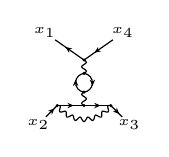
\begin{tikzpicture}[x=0.340cm, y=0.340cm, line width=0.420pt, baseline={([yshift=-0.6ex]0,0)}]
  \draw (0.000,-0.567) -- (1.000,-0.567);
  \fill (0.619,-0.567) -- (0.381,-0.465) -- (0.458,-0.567) -- (0.381,-0.669) -- cycle;
  \draw (-1.000,-0.567) -- (0.000,-0.567);
  \fill (-0.381,-0.567) -- (-0.619,-0.465) -- (-0.542,-0.567) -- (-0.619,-0.669) -- cycle;
  \draw (0.000,-0.067) arc[start angle=263.974, end angle=96.026, radius=0.352];
  \fill (-0.315,0.403) -- (-0.417,0.164) -- (-0.315,0.242) -- (-0.213,0.164) -- cycle;
  \draw (0.000,0.633) arc[start angle=83.974, end angle=-83.974, radius=0.352];
  \fill (0.315,0.164) -- (0.417,0.403) -- (0.315,0.325) -- (0.213,0.403) -- cycle;
  \draw plot[smooth, tension=0.7] coordinates {(0.000,1.133) (0.064,1.092) (0.090,1.050) (0.064,1.008) (0.000,0.967) (-0.064,0.925) (-0.090,0.883) (-0.064,0.842) (0.000,0.800) (0.064,0.758) (0.090,0.717) (0.064,0.675) (0.000,0.633)};
  \draw plot[smooth, tension=0.7] coordinates {(-1.000,-0.567) (-0.931,-0.564) (-0.890,-0.578) (-0.885,-0.622) (-0.902,-0.688) (-0.917,-0.757) (-0.904,-0.803) (-0.858,-0.814) (-0.790,-0.797) (-0.724,-0.777) (-0.680,-0.780) (-0.664,-0.821) (-0.665,-0.890) (-0.661,-0.960) (-0.638,-1.001) (-0.590,-1.000) (-0.529,-0.966) (-0.470,-0.930) (-0.427,-0.923) (-0.401,-0.958) (-0.384,-1.025) (-0.363,-1.092) (-0.330,-1.126) (-0.284,-1.112) (-0.233,-1.064) (-0.185,-1.014) (-0.145,-0.996) (-0.111,-1.024) (-0.078,-1.084) (-0.041,-1.143) (0.000,-1.168) (0.041,-1.143) (0.078,-1.084) (0.111,-1.024) (0.145,-0.996) (0.185,-1.014) (0.233,-1.064) (0.284,-1.112) (0.330,-1.126) (0.363,-1.092) (0.384,-1.025) (0.401,-0.958) (0.427,-0.923) (0.470,-0.930) (0.529,-0.966) (0.590,-1.000) (0.638,-1.001) (0.661,-0.960) (0.665,-0.890) (0.664,-0.821) (0.680,-0.780) (0.724,-0.777) (0.790,-0.797) (0.858,-0.814) (0.904,-0.803) (0.917,-0.757) (0.902,-0.688) (0.885,-0.622) (0.890,-0.578) (0.931,-0.564) (1.000,-0.567)};
  \draw plot[smooth, tension=0.7] coordinates {(0.000,-0.567) (-0.064,-0.525) (-0.090,-0.483) (-0.064,-0.442) (0.000,-0.400) (0.064,-0.358) (0.090,-0.317) (0.064,-0.275) (0.000,-0.233) (-0.064,-0.192) (-0.090,-0.150) (-0.064,-0.108) (0.000,-0.067)};
  \draw (0.000,1.133) -- (-1.081,1.890);
  \fill (-0.693,1.618) -- (-0.555,1.398) -- (-0.560,1.526) -- (-0.438,1.565) -- cycle;
  \draw (-1.000,-0.567) -- (-1.424,-0.991);
  \fill (-1.106,-0.673) -- (-1.347,-0.770) -- (-1.220,-0.787) -- (-1.203,-0.914) -- cycle;
  \draw (1.000,-0.567) -- (1.424,-0.991);
  \fill (1.318,-0.884) -- (1.221,-0.643) -- (1.204,-0.770) -- (1.077,-0.788) -- cycle;
  \draw (0.000,1.133) -- (1.081,1.890);
  \fill (0.389,1.406) -- (0.643,1.459) -- (0.521,1.498) -- (0.526,1.626) -- cycle;
  \fill (0.000,1.133) circle (0.064);
  \fill (-1.000,-0.567) circle (0.064);
  \fill (1.000,-0.567) circle (0.064);
  \fill (0.000,-0.567) circle (0.064);
  \fill (0.000,0.633) circle (0.064);
  \fill (0.000,-0.067) circle (0.064);
  \node[font=\tiny, inner sep=0pt, anchor=325] at (-1.155,1.942) {$x_{1}$};
  \node[font=\tiny, inner sep=0pt, anchor=45] at (-1.488,-1.055) {$x_{2}$};
  \node[font=\tiny, inner sep=0pt, anchor=135] at (1.488,-1.055) {$x_{3}$};
  \node[font=\tiny, inner sep=0pt, anchor=215] at (1.155,1.942) {$x_{4}$};
\end{tikzpicture}}
\diagramgap
\mbox{$\displaystyle -\,$\,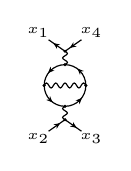
\begin{tikzpicture}[x=0.340cm, y=0.340cm, line width=0.420pt, baseline={([yshift=-0.6ex]0,0)}]
  \draw (0.778,0.000) arc[start angle=360.000, end angle=450.000, radius=0.778];
  \fill (0.466,0.634) -- (0.562,0.393) -- (0.580,0.520) -- (0.707,0.538) -- cycle;
  \draw (-0.778,0.000) arc[start angle=180.000, end angle=270.000, radius=0.778];
  \fill (-0.466,-0.634) -- (-0.562,-0.393) -- (-0.580,-0.520) -- (-0.707,-0.538) -- cycle;
  \draw (0.000,0.778) arc[start angle=90.000, end angle=180.000, radius=0.778];
  \fill (-0.634,0.466) -- (-0.393,0.562) -- (-0.520,0.580) -- (-0.538,0.707) -- cycle;
  \draw (0.000,-0.778) arc[start angle=270.000, end angle=360.000, radius=0.778];
  \fill (0.634,-0.466) -- (0.393,-0.562) -- (0.520,-0.580) -- (0.538,-0.707) -- cycle;
  \draw plot[smooth, tension=0.7] coordinates {(0.000,1.278) (0.064,1.236) (0.090,1.194) (0.064,1.153) (0.000,1.111) (-0.064,1.069) (-0.090,1.028) (-0.064,0.986) (0.000,0.944) (0.064,0.903) (0.090,0.861) (0.064,0.819) (0.000,0.778)};
  \draw plot[smooth, tension=0.7] coordinates {(0.000,-1.278) (-0.064,-1.236) (-0.090,-1.194) (-0.064,-1.153) (0.000,-1.111) (0.064,-1.069) (0.090,-1.028) (0.064,-0.986) (0.000,-0.944) (-0.064,-0.903) (-0.090,-0.861) (-0.064,-0.819) (0.000,-0.778)};
  \draw plot[smooth, tension=0.7] coordinates {(-0.778,0.000) (-0.735,0.066) (-0.691,0.093) (-0.648,0.066) (-0.605,0.000) (-0.562,-0.066) (-0.519,-0.093) (-0.475,-0.066) (-0.432,0.000) (-0.389,0.066) (-0.346,0.093) (-0.302,0.066) (-0.259,0.000) (-0.216,-0.066) (-0.173,-0.093) (-0.130,-0.066) (-0.086,0.000) (-0.043,0.066) (0.000,0.093) (0.043,0.066) (0.086,0.000) (0.130,-0.066) (0.173,-0.093) (0.216,-0.066) (0.259,0.000) (0.302,0.066) (0.346,0.093) (0.389,0.066) (0.432,0.000) (0.475,-0.066) (0.519,-0.093) (0.562,-0.066) (0.605,0.000) (0.648,0.066) (0.691,0.093) (0.735,0.066) (0.778,0.000)};
  \draw (0.000,1.278) -- (-0.614,1.708);
  \fill (-0.436,1.583) -- (-0.299,1.362) -- (-0.304,1.490) -- (-0.182,1.530) -- cycle;
  \draw (0.000,-1.278) -- (-0.614,-1.708);
  \fill (-0.179,-1.403) -- (-0.433,-1.456) -- (-0.311,-1.495) -- (-0.316,-1.623) -- cycle;
  \draw (0.000,-1.278) -- (0.614,-1.708);
  \fill (0.436,-1.583) -- (0.299,-1.362) -- (0.304,-1.490) -- (0.182,-1.530) -- cycle;
  \draw (0.000,1.278) -- (0.614,1.708);
  \fill (0.179,1.403) -- (0.433,1.456) -- (0.311,1.495) -- (0.316,1.623) -- cycle;
  \fill (0.000,1.278) circle (0.064);
  \fill (0.000,-1.278) circle (0.064);
  \fill (0.000,0.778) circle (0.064);
  \fill (0.000,-0.778) circle (0.064);
  \fill (-0.778,0.000) circle (0.064);
  \fill (0.778,0.000) circle (0.064);
  \node[font=\tiny, inner sep=0pt, anchor=325] at (-0.688,1.760) {$x_{1}$};
  \node[font=\tiny, inner sep=0pt, anchor=35] at (-0.688,-1.760) {$x_{2}$};
  \node[font=\tiny, inner sep=0pt, anchor=145] at (0.688,-1.760) {$x_{3}$};
  \node[font=\tiny, inner sep=0pt, anchor=215] at (0.688,1.760) {$x_{4}$};
\end{tikzpicture}}
\diagramgap
\mbox{$\displaystyle +\,$\,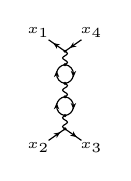
\begin{tikzpicture}[x=0.340cm, y=0.340cm, line width=0.420pt, baseline={([yshift=-0.6ex]0,0)}]
  \draw (0.000,0.250) arc[start angle=263.974, end angle=96.026, radius=0.352];
  \fill (-0.315,0.719) -- (-0.417,0.481) -- (-0.315,0.558) -- (-0.213,0.481) -- cycle;
  \draw (0.000,0.950) arc[start angle=83.974, end angle=-83.974, radius=0.352];
  \fill (0.315,0.481) -- (0.417,0.719) -- (0.315,0.642) -- (0.213,0.719) -- cycle;
  \draw (0.000,-0.250) arc[start angle=83.974, end angle=-83.974, radius=0.352];
  \fill (0.315,-0.719) -- (0.417,-0.481) -- (0.315,-0.558) -- (0.213,-0.481) -- cycle;
  \draw (0.000,-0.950) arc[start angle=263.974, end angle=96.026, radius=0.352];
  \fill (-0.315,-0.481) -- (-0.417,-0.719) -- (-0.315,-0.642) -- (-0.213,-0.719) -- cycle;
  \draw plot[smooth, tension=0.7] coordinates {(0.000,1.450) (0.064,1.408) (0.090,1.367) (0.064,1.325) (0.000,1.283) (-0.064,1.242) (-0.090,1.200) (-0.064,1.158) (0.000,1.117) (0.064,1.075) (0.090,1.033) (0.064,0.992) (0.000,0.950)};
  \draw plot[smooth, tension=0.7] coordinates {(0.000,-1.450) (-0.064,-1.408) (-0.090,-1.367) (-0.064,-1.325) (0.000,-1.283) (0.064,-1.242) (0.090,-1.200) (0.064,-1.158) (0.000,-1.117) (-0.064,-1.075) (-0.090,-1.033) (-0.064,-0.992) (0.000,-0.950)};
  \draw plot[smooth, tension=0.7] coordinates {(0.000,0.250) (0.064,0.208) (0.090,0.167) (0.064,0.125) (0.000,0.083) (-0.064,0.042) (-0.090,0.000) (-0.064,-0.042) (0.000,-0.083) (0.064,-0.125) (0.090,-0.167) (0.064,-0.208) (0.000,-0.250)};
  \draw (0.000,1.450) -- (-0.614,1.880);
  \fill (-0.436,1.755) -- (-0.299,1.535) -- (-0.304,1.663) -- (-0.182,1.702) -- cycle;
  \draw (0.000,-1.450) -- (-0.614,-1.880);
  \fill (-0.179,-1.575) -- (-0.433,-1.628) -- (-0.311,-1.668) -- (-0.316,-1.796) -- cycle;
  \draw (0.000,-1.450) -- (0.614,-1.880);
  \fill (0.436,-1.755) -- (0.299,-1.535) -- (0.304,-1.663) -- (0.182,-1.702) -- cycle;
  \draw (0.000,1.450) -- (0.614,1.880);
  \fill (0.179,1.575) -- (0.433,1.628) -- (0.311,1.668) -- (0.316,1.796) -- cycle;
  \fill (0.000,1.450) circle (0.064);
  \fill (0.000,-1.450) circle (0.064);
  \fill (0.000,0.950) circle (0.064);
  \fill (0.000,-0.950) circle (0.064);
  \fill (0.000,0.250) circle (0.064);
  \fill (0.000,-0.250) circle (0.064);
  \node[font=\tiny, inner sep=0pt, anchor=325] at (-0.688,1.932) {$x_{1}$};
  \node[font=\tiny, inner sep=0pt, anchor=35] at (-0.688,-1.932) {$x_{2}$};
  \node[font=\tiny, inner sep=0pt, anchor=145] at (0.688,-1.932) {$x_{3}$};
  \node[font=\tiny, inner sep=0pt, anchor=215] at (0.688,1.932) {$x_{4}$};
\end{tikzpicture}}
